% Options for packages loaded elsewhere
\PassOptionsToPackage{unicode}{hyperref}
\PassOptionsToPackage{hyphens}{url}
%
\documentclass[
]{article}
\usepackage{amsmath,amssymb}
\usepackage{lmodern}
\usepackage{ifxetex,ifluatex}
\ifnum 0\ifxetex 1\fi\ifluatex 1\fi=0 % if pdftex
  \usepackage[T1]{fontenc}
  \usepackage[utf8]{inputenc}
  \usepackage{textcomp} % provide euro and other symbols
\else % if luatex or xetex
  \usepackage{unicode-math}
  \defaultfontfeatures{Scale=MatchLowercase}
  \defaultfontfeatures[\rmfamily]{Ligatures=TeX,Scale=1}
\fi
% Use upquote if available, for straight quotes in verbatim environments
\IfFileExists{upquote.sty}{\usepackage{upquote}}{}
\IfFileExists{microtype.sty}{% use microtype if available
  \usepackage[]{microtype}
  \UseMicrotypeSet[protrusion]{basicmath} % disable protrusion for tt fonts
}{}
\makeatletter
\@ifundefined{KOMAClassName}{% if non-KOMA class
  \IfFileExists{parskip.sty}{%
    \usepackage{parskip}
  }{% else
    \setlength{\parindent}{0pt}
    \setlength{\parskip}{6pt plus 2pt minus 1pt}}
}{% if KOMA class
  \KOMAoptions{parskip=half}}
\makeatother
\usepackage{xcolor}
\IfFileExists{xurl.sty}{\usepackage{xurl}}{} % add URL line breaks if available
\IfFileExists{bookmark.sty}{\usepackage{bookmark}}{\usepackage{hyperref}}
\hypersetup{
  hidelinks,
  pdfcreator={LaTeX via pandoc}}
\urlstyle{same} % disable monospaced font for URLs
\usepackage[margin=1in]{geometry}
\usepackage{longtable,booktabs,array}
\usepackage{calc} % for calculating minipage widths
% Correct order of tables after \paragraph or \subparagraph
\usepackage{etoolbox}
\makeatletter
\patchcmd\longtable{\par}{\if@noskipsec\mbox{}\fi\par}{}{}
\makeatother
% Allow footnotes in longtable head/foot
\IfFileExists{footnotehyper.sty}{\usepackage{footnotehyper}}{\usepackage{footnote}}
\makesavenoteenv{longtable}
\usepackage{graphicx}
\makeatletter
\def\maxwidth{\ifdim\Gin@nat@width>\linewidth\linewidth\else\Gin@nat@width\fi}
\def\maxheight{\ifdim\Gin@nat@height>\textheight\textheight\else\Gin@nat@height\fi}
\makeatother
% Scale images if necessary, so that they will not overflow the page
% margins by default, and it is still possible to overwrite the defaults
% using explicit options in \includegraphics[width, height, ...]{}
\setkeys{Gin}{width=\maxwidth,height=\maxheight,keepaspectratio}
% Set default figure placement to htbp
\makeatletter
\def\fps@figure{htbp}
\makeatother
\setlength{\emergencystretch}{3em} % prevent overfull lines
\providecommand{\tightlist}{%
  \setlength{\itemsep}{0pt}\setlength{\parskip}{0pt}}
\setcounter{secnumdepth}{5}
\usepackage{booktabs}
\usepackage{booktabs}
\usepackage{longtable}
\usepackage{array}
\usepackage{multirow}
\usepackage{wrapfig}
\usepackage{float}
\usepackage{colortbl}
\usepackage{pdflscape}
\usepackage{tabu}
\usepackage{threeparttable}
\usepackage{threeparttablex}
\usepackage[normalem]{ulem}
\usepackage{makecell}
\usepackage{xcolor}
\ifluatex
  \usepackage{selnolig}  % disable illegal ligatures
\fi
\usepackage[]{natbib}
\bibliographystyle{plainnat}

\author{}
\date{\vspace{-2.5em}}

\begin{document}

{
\setcounter{tocdepth}{2}
\tableofcontents
}
\hypertarget{intro}{%
\section{Introduction}\label{intro}}

The objective of this textbook is to provide you with the shortest path to exploring your data, visualizing it, forming hypotheses and validating and defending them. Given a data set, you want to be able to make any plot you wish, find plots which show something actionable and interesting, explore data by slicing and dicing it and finally present your results in a statistically convincing manner, perhaps in a colorful and visually appealing way.

Questions which you will have to anticipate and you will have to answer are
- How do you know that your findings are not random?
- And fundamental of all questions:
- \textbf{So what?}

Even the most impressing looking results may come up randomly. And you will be asked this question along with the question \emph{``what was your p-value and how did you compute it''}

And even if you convince your audience that your results are not random, you will have to be ready to explain why your audience should care about the results you reported. In other words, is there any actionable value in your results? Or they are just simply interesting, good to know, but no one really needs to care much about them otherwise? Hopefully it is the former not the latter.

In the following sections we will address these questions and go through the process of data exploration, validation, and presentation.

\begin{itemize}
\tightlist
\item
  We will start with making plots, follow with free style data exploration -- which allows us to form the leads, that is hypotheses. Then we will follow with simple statistical tests which will allow us to validate these hypothesis and defend our findings against randomness claims. - We will learn how to calculate p-values and how to use them to defend our findings.
\item
  We will use as few R commands as possible and reach our goal in the shortest possible path. In fact we will demonstrate how using just 7 R commands we can perform quite sophisticated data exploration. In the appendix, we show many more useful commands of R which eventually you would have to use. However, our goal in this short textbook, is to present the shortest path to data analysis which will let you import the data, plot it, make some analysis yourself and use R-libraries. In this textbook and in this class we do not teach how to clean the data (data wrangling) and how to deal with a wide variety of data types. We also do not address complex data transformations such as multi-frame operations like merge (we show them in appendix). We also do not explain how different machine learning methods work, we only show you how to use them. It is similar to teaching one how to drive a car without knowing how a car engine works.
\end{itemize}

\hypertarget{b2022}{%
\section{🔖 Best Works of 2022}\label{b2022}}

\hypertarget{datablog}{%
\subsection{DataBlog}\label{datablog}}

Ella Walmsley

\hypertarget{bt12}{}

\hypertarget{prediction-challenge-1}{%
\subsection{Prediction Challenge 1}\label{prediction-challenge-1}}

Upsham Naik

Jeevanandan Ramasamy

\hypertarget{bt15}{}

\hypertarget{bt13}{}

\hypertarget{prediction-challenge-2}{%
\subsection{Prediction Challenge 2}\label{prediction-challenge-2}}

Jeevanandan Ramasamy

\hypertarget{bt14}{}

\hypertarget{DLL}{%
\section{Data League Leaderboard}\label{DLL}}

\begin{table}

\caption{\label{tab:unnamed-chunk-4}Leaderboard 2022}
\centering
\begin{tabular}[t]{rl}
\toprule
Rank & Participant.Name\\
\midrule
1 & Jeevanandan Ramasamy\\
2 & George Basta\\
3 & Joyce Huang\\
4 & Jiaxu Hu\\
5 & Dhiren Patel\\
\addlinespace
6 & Chicheng Shao\\
7 & Cheyenne Pourkay\\
8 & Christopher Nguyen\\
9 & Aaron Mok\\
10 & Ethan Matta\\
\bottomrule
\end{tabular}
\end{table}

\textbf{Honourable Mentions: }
Upsham Naik, Joshua B. Sze, Kirtan Patel, Maria Xu, Devam Patel, Eva Zhang, Toshanraju Vysyaraju, Maanas Pimplikar, Jared Chiou, Nitya Narayanan, Shrish Vellore, Yousra Belgaid, Mitali Shroff, Michael Jucan, Jackie Hong, Arvin Sung, Eric Xuan, Eva Allred, Leah Ranavat, Nami Jain, Gautam Agarwal, Aditya Patil

\hypertarget{data-puzzles-secrets}{%
\section{🔖 Data puzzles secrets}\label{data-puzzles-secrets}}

\begin{itemize}
\tightlist
\item
  \textbf{Lecture slides: } Data Exploration

  \hypertarget{freestyle12}{}
\end{itemize}

\hypertarget{moody-data-puzzle}{%
\subsection{Moody Data Puzzle}\label{moody-data-puzzle}}

\begin{table}

\caption{\label{tab:unnamed-chunk-6}Snippet of Moody Dataset}
\centering
\begin{tabular}[t]{rlllr}
\toprule
SCORE & GRADE & DOZES\_OFF & TEXTING\_IN\_CLASS & PARTICIPATION\\
\midrule
21.33 & F & never & never & 0.29\\
71.57 & C & always & rarely & 0.11\\
90.11 & A & always & never & 0.26\\
31.52 & D & sometimes & rarely & 0.03\\
95.94 & A & always & rarely & 0.21\\
\bottomrule
\end{tabular}
\end{table}

Moody Data Puzzle is our first example of a data puzzle. By data puzzles we mean synthetically generated data sets which have some embedded patterns. Your goal is to find the embedded pattern(s). You may also find patterns similar (implied) by patterns embedded in the data puzzle. This is fine too. The goal of data puzzles is to excite you about exploratory data analysis. In many ways it is like a game.

\textbf{Puzzle description:}

Professor Moody has been teaching statistics 101 class for many years. His teaching evaluations went considerably south with the chief complaint: he DOES NOT seem to assign grades fairly. Students compared their scores among themselves and found quite a bit of discrepancies! But their complaints went nowhere since Professor promptly disappeared after posting the final grades and scores.

A new brave TA, managed to get hold of the carefully maintained grading table (spanning multiple years) of professor Moody by \ldots.messing a bit with Moody's computer\ldots.well, let's not explain the details because he would get in trouble. What he found out was a remarkably structured account of how professor Moody assigns his grades.

Looks like Professor Moody is in fact very alert in class. He is aware of what students do, detecting texting during class and remembering exactly who was dozed off in class. He also keeps the mysterious ``participation index'' which is a numerical score from 0 to 1. This is probably related to questions asked and answered by students as well as their general attentiveness in class. Remarkable but a little creepy, isn't it?

What is the best advice the new TA, can give future students how to get a good grade in Professor Moody's class? What factors influence the grade besides the score? Back your recommendation up with plots and evidence from the attached data.

\textbf{What are examples of patterns we are looking for here?}

Here are some:

\begin{itemize}
\tightlist
\item
  ``Students who text a lot'' have lower chance to get an A in the class''
\item
  ``Students whose participation is lower than 0.25 fail the class more often''
\item
  ``Dozing off does not matter if your score is more than 90, you still get an A''
\item
  ``If you score is less than 30, you fail the class regardless of what your other attributes are''
\end{itemize}

\hypertarget{secrets-revealed--patterns-in-professor-moodys-data}{%
\subsubsection{Secrets Revealed- Patterns in Professor Moody's data?}\label{secrets-revealed--patterns-in-professor-moodys-data}}

My Patterns

\hypertarget{MDP12}{}

Many student solutions falsely attribute higher grades to higher values of participation attribute..

This is a classic example of a hidden variable described in the reference attached below.

The truth is that participation attribute value impacts the score attribute value. Generally, the higher the participation in Moody's class, the higher the score. But it is the score attribute which has a direct impact on the grade. Thus, it is the score which is the real ``hidden variable'' impacting the final grade.

Thus, the score already reflects participation. Professor Moody seemed to look only at texting and dozing off attributes in grade determination (see the power points above with the explanation)

Compare with examples of hidden variables in the following reference about correlation and causation.

\url{https://www.stewartmath.com/precalc_7e_dp/precalc_7e_dp6.html}

\hypertarget{best-students-submissions-2022}{%
\subsubsection{Best Student's Submissions 2022}\label{best-students-submissions-2022}}

Lauretta Martin

Sanjaya Budhathoki

Sandhya Senthilkumar

\hypertarget{PPT2021}{}

\hypertarget{PPT2020}{}

\hypertarget{PPT2019}{}

\hypertarget{movies-data-hunt}{%
\subsection{Movies Data Hunt}\label{movies-data-hunt}}

\begin{table}

\caption{\label{tab:unnamed-chunk-19}Snippet of Movies Dataset}
\centering
\begin{tabular}[t]{lllrlll}
\toprule
  & country & content & imdb\_score & Gross & Budget & genre\\
\midrule
9543 & USA & PG-13 & 7.32 & Low & Medium & History\\
7319 & USA & PG-13 & 6.91 & Low & Medium & Drama\\
583 & USA & PG-13 & 7.48 & High & High & Drama\\
11604 & USA & PG-13 & 6.62 & Low & Low & History\\
544 & USA & PG-13 & 6.08 & High & High & Family\\
\bottomrule
\end{tabular}
\end{table}

\textbf{Puzzle description:}

contains imdb scores of 12,800+ movies along with several attributes including budget, gross genre, content rating etc.

What are the most promising alternative hypotheses about imdb scores to test? Name your three top candidates along with the evidence which backs them up: either in the form of R instruction(s) or plot.

\hypertarget{secrets-revealed--patterns-in-movies-data}{%
\subsubsection{Secrets Revealed- Patterns in Movies data?}\label{secrets-revealed--patterns-in-movies-data}}

Secrets Revealed

\hypertarget{MV12}{}

\hypertarget{best-students-submissions-2022-1}{%
\subsubsection{Best Student's Submissions 2022}\label{best-students-submissions-2022-1}}

Joshua Sze

Andrew Fasano

\hypertarget{hw41}{}

\hypertarget{hw42}{}

\hypertarget{minimarket-data-hunt}{%
\subsection{Minimarket Data Hunt}\label{minimarket-data-hunt}}

\begin{table}

\caption{\label{tab:unnamed-chunk-20}Snippet of Minimarket Dataset}
\centering
\begin{tabular}[t]{lrrrrr}
\toprule
  & BREAD & BUTTER & COOKIES & COFFEE & TEA\\
\midrule
8348 & 1 & 1 & 1 & 1 & 1\\
8599 & 0 & 1 & 0 & 0 & 0\\
8537 & 1 & 0 & 0 & 1 & 0\\
4826 & 0 & 1 & 0 & 0 & 1\\
7153 & 0 & 1 & 1 & 1 & 1\\
\bottomrule
\end{tabular}
\end{table}

\textbf{Puzzle description:}

Each row of Minimarket.csv contains one customer transaction which is represented as binary vector (treat this as NUM values). 1 means that customer bought an item, 0 - means that customer did not but that item. For example if customer bought Bread but did not buy Butter you will see 1 in the Bread column and 0 in the Butter column.

\textbf{Summary}

Here's what you'd do:
1. Come up with a null hypothesis: ``Bread does not impact the sales of butter''
2. Come up with an alternative hypothesis: ``Bread impacts the sale of butter''
3. Compute the mean value of the Butter column for all the rows where Bread value = 0. Let's say this is mean1.
4. Compute the mean value of the Butter column for all the rows where Bread value = 1. Let's say this is mean2.

\hypertarget{what-were-the-secret-associations-between-items-in-the-minimarket}{%
\subsubsection{What were the secret associations between items in the minimarket?}\label{what-were-the-secret-associations-between-items-in-the-minimarket}}

Secrets Revealed

\hypertarget{MV12}{}

\hypertarget{predicting-grades-in-professor-moodys-class}{%
\subsection{Predicting grades in Professor Moody's class}\label{predicting-grades-in-professor-moodys-class}}

\hypertarget{how-did-i-cook-the-professor-moody-prediction-challenge-data}{%
\subsubsection{How did I cook the Professor Moody Prediction challenge data?}\label{how-did-i-cook-the-professor-moody-prediction-challenge-data}}

Secrets Revealed

\hypertarget{MV13}{}

\hypertarget{setting-up-r}{%
\section{Setting Up R}\label{setting-up-r}}

\begin{itemize}
\item
  \textbf{Important Instructions}

  \begin{itemize}
  \tightlist
  \item
    Installation of R is required before installing RStudio

    \begin{itemize}
    \tightlist
    \item
      ``R'' is a programming language, and,
    \item
      ``RStudio'' is an Integrated Development Environment (IDE) which provides you a platform to code in R.
    \end{itemize}
  \end{itemize}
\item
  \textbf{How to download and install R \& RStudio?}

  \begin{itemize}
  \item
    \emph{Downloading and installing R.}

    \begin{itemize}
    \tightlist
    \item
      For Windows Users.

      \begin{itemize}
      \tightlist
      \item
        Click on the link provided below or copy paste it on your favourite browser and go to the website.

        \begin{itemize}
        \tightlist
        \item
          \url{https://cran.r-project.org/bin/windows/base/}
        \end{itemize}
      \item
        Click on the link at top left where it says ``Download R 4.0.3 for windows'' or the latest at the time of your installation.
      \item
        Open the downloaded file and follow the instructions as it is.
      \end{itemize}
    \item
      For MAC Users.

      \begin{itemize}
      \tightlist
      \item
        Click on the link provided below or copy paste it on your favourite browser and go to the website.

        \begin{itemize}
        \tightlist
        \item
          \url{https://cloud.r-project.org/bin/macosx/}
        \end{itemize}
      \item
        Under ``Latest release'', click on ``R-4.0.3.pkg'' or the latest at the time of your installation.
      \item
        Open the downloaded file and follow the instructions as it is.
      \end{itemize}
    \end{itemize}
  \item
    \emph{Downloading and installing RStudio.}

    \begin{itemize}
    \tightlist
    \item
      For Windows Users.

      \begin{itemize}
      \tightlist
      \item
        Click on the link below or copy paste it in your favourite browser.

        \begin{itemize}
        \tightlist
        \item
          \url{https://rstudio.com/products/rstudio/download/}
        \end{itemize}
      \item
        Scroll down almost till the end of the web page until you find a section named ``All Installers''.
      \item
        Click on the download link beside ``Windows 10/8/7'' to download the windows version of RStudio.
      \item
        Install RStudio by clicking on the downloaded file and following the instructions as it is.
      \end{itemize}
    \item
      For MAC Users.

      \begin{itemize}
      \tightlist
      \item
        Click on the link below or copy paste it in your favourite browser.

        \begin{itemize}
        \tightlist
        \item
          \url{https://rstudio.com/products/rstudio/download/}
        \end{itemize}
      \item
        Scroll down almost till the end of the web page until you find a section named ``All Installers''.
      \item
        Click on the link beside ``macOS 10.13+'' to start your download the MAC version of RStudio.
      \item
        Install RStudio by clicking on the downloaded file and following the instructions as it is.
      \end{itemize}
    \end{itemize}
  \end{itemize}
\end{itemize}

\begin{center}\rule{0.5\linewidth}{0.5pt}\end{center}

\hypertarget{setting}{%
\subsection{Create New Project}\label{setting}}

After installing R studio successfully the first step is to create a project R studio.

\begin{itemize}
\tightlist
\item
  Step 1: Go to \textbf{File -\textgreater{} New Project}
\end{itemize}

\begin{figure}
\centering
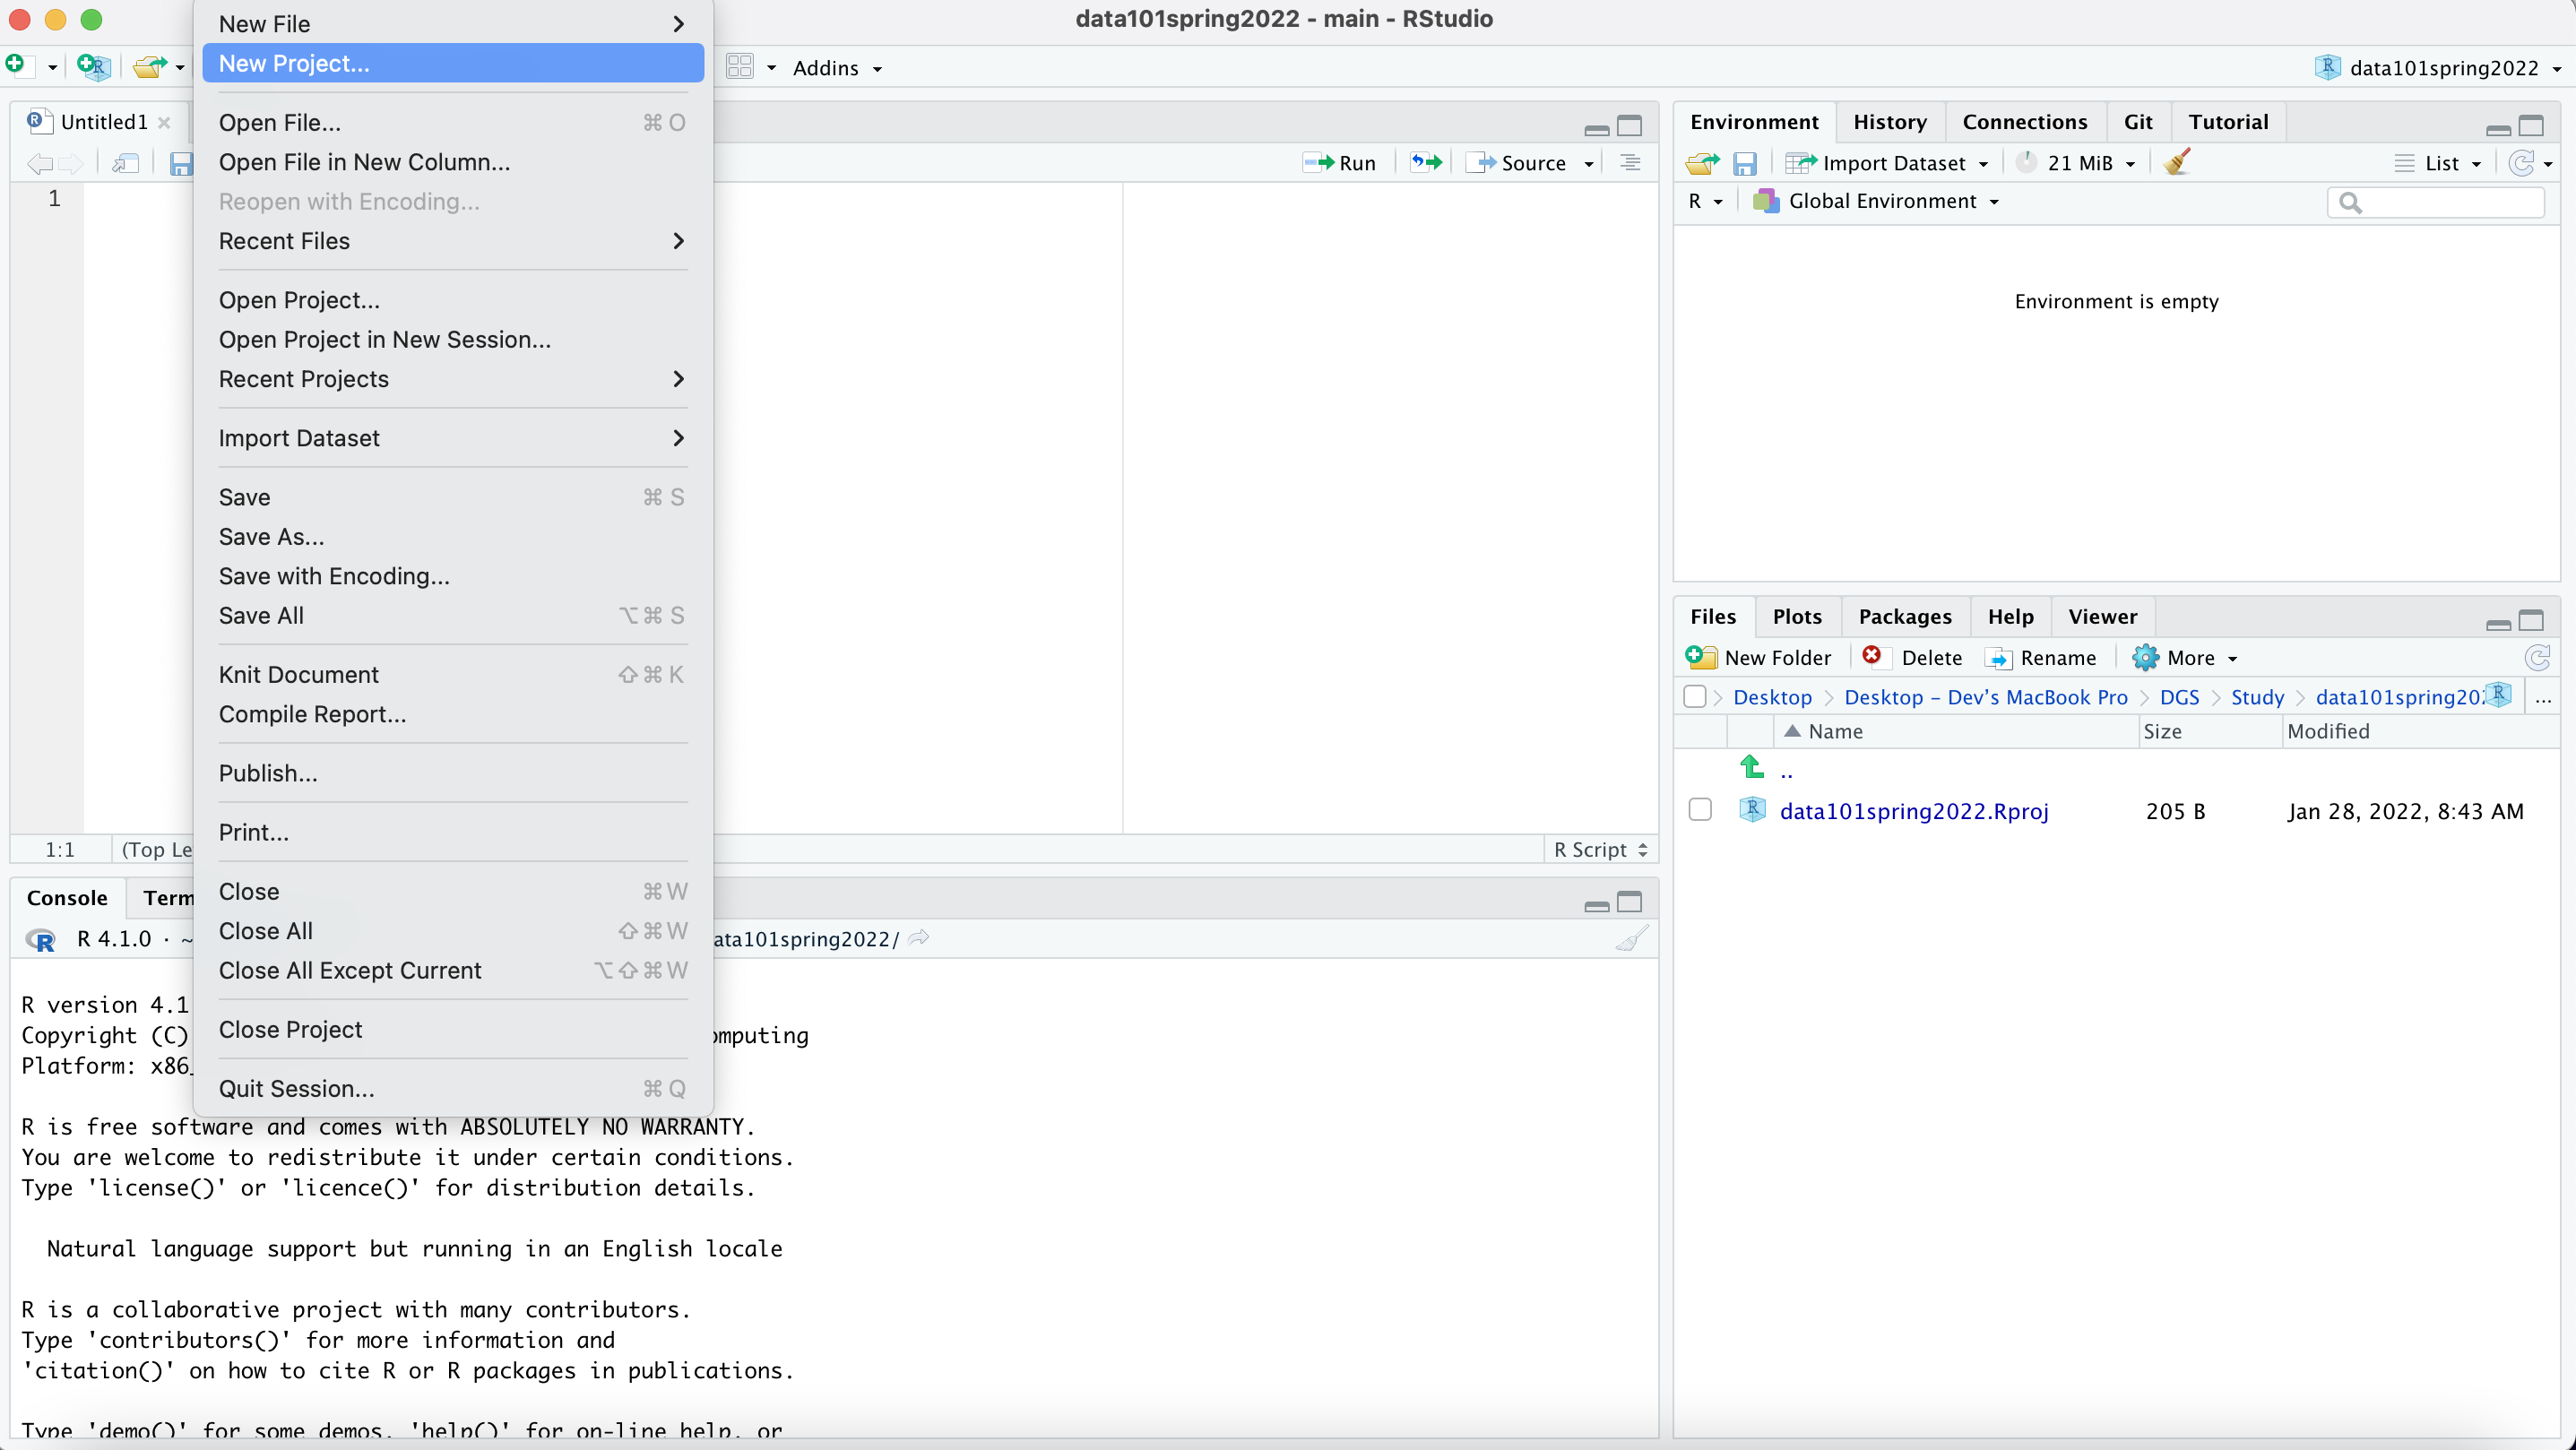
\includegraphics{https://raw.githubusercontent.com/dev7796/data101_tutorial/main/files/img/plots/1_text.png}
\caption{New Project}
\end{figure}

\begin{itemize}
\tightlist
\item
  Step 2: Select \textbf{New Directory}
\end{itemize}

\begin{figure}
\centering
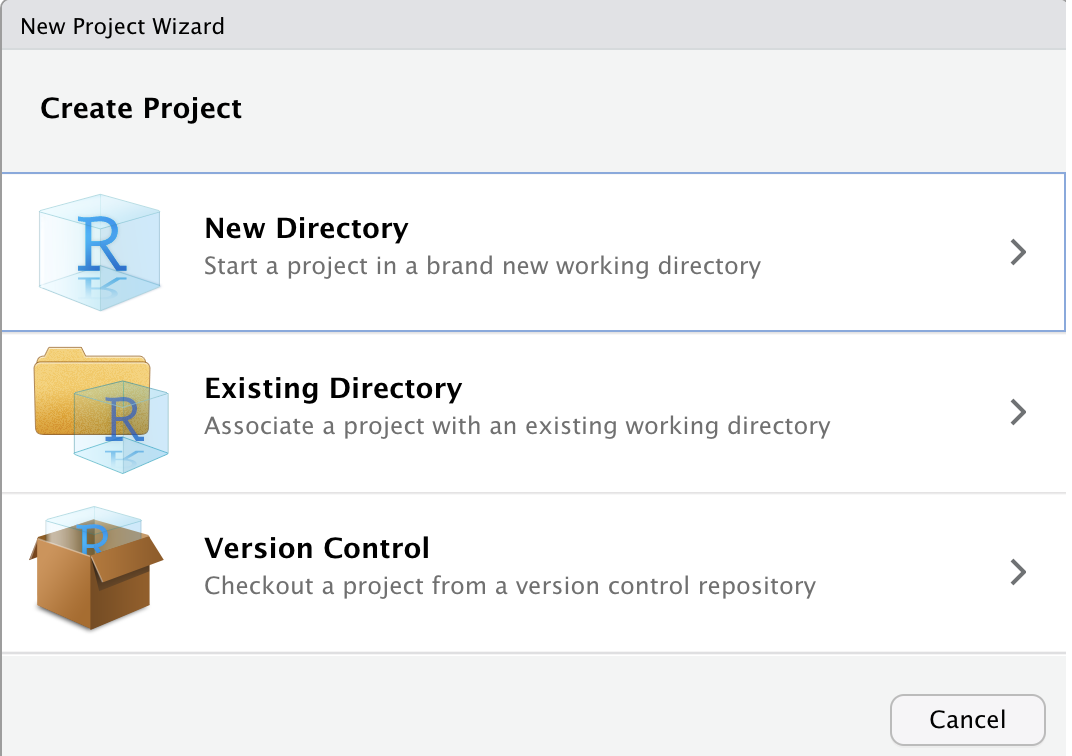
\includegraphics{https://raw.githubusercontent.com/dev7796/data101_tutorial/main/files/img/plots/2_text.png}
\caption{New Directory}
\end{figure}

\begin{itemize}
\tightlist
\item
  Step 3: Select \textbf{New Project}
\end{itemize}

\begin{figure}
\centering
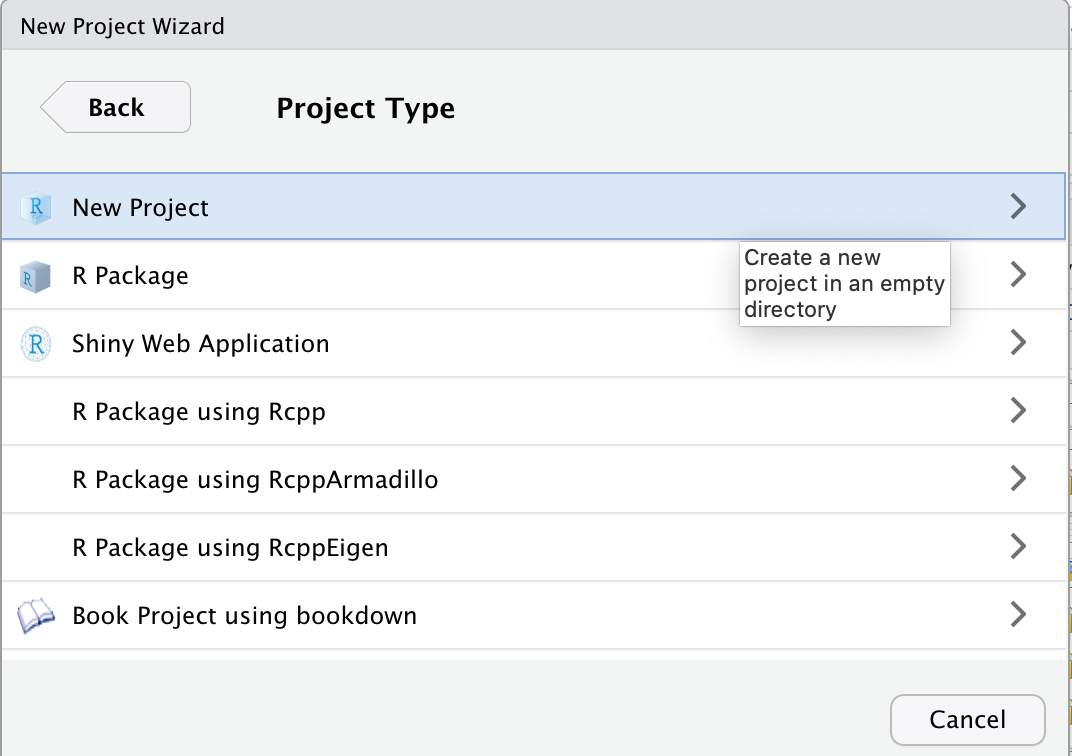
\includegraphics{https://raw.githubusercontent.com/dev7796/data101_tutorial/main/files/img/plots/3_text.png}
\caption{New Project}
\end{figure}

\begin{itemize}
\tightlist
\item
  Step 4: Give your preferred directory name like \textbf{``Data101\_Assignmnets''}
\end{itemize}

\begin{figure}
\centering
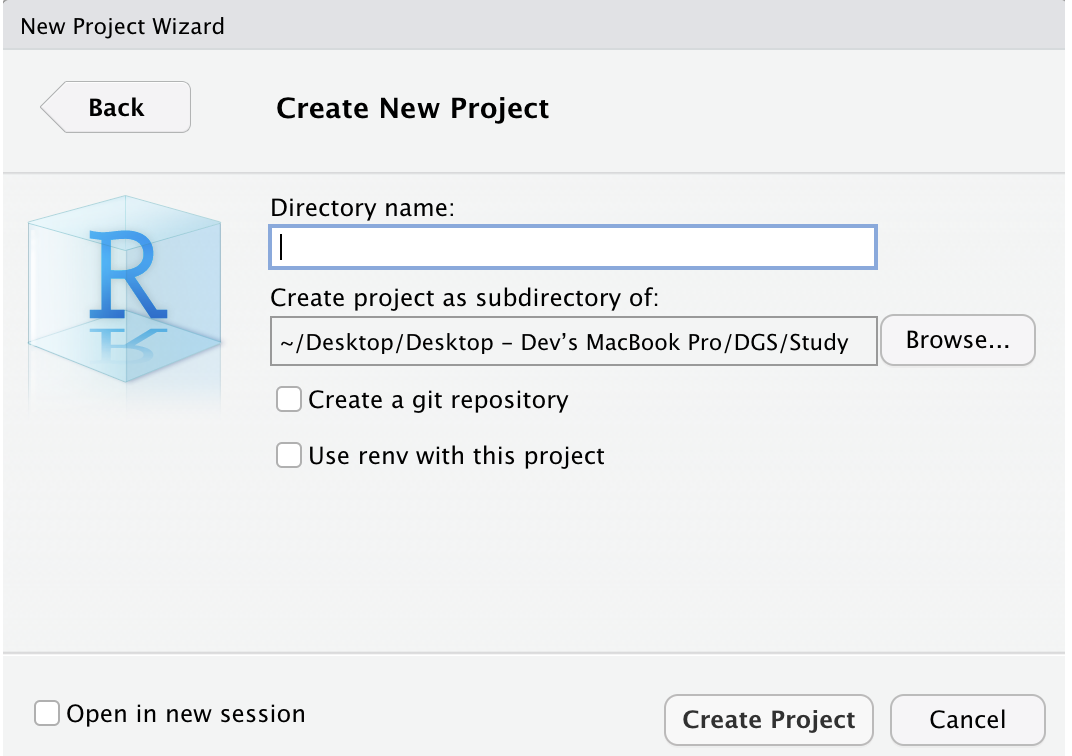
\includegraphics{https://raw.githubusercontent.com/dev7796/data101_tutorial/main/files/img/plots/4_text.png}
\caption{Directory Name}
\end{figure}

\begin{itemize}
\tightlist
\item
  Step 5: Click on Create Project and finally the R studio should look like
\end{itemize}

\begin{figure}
\centering
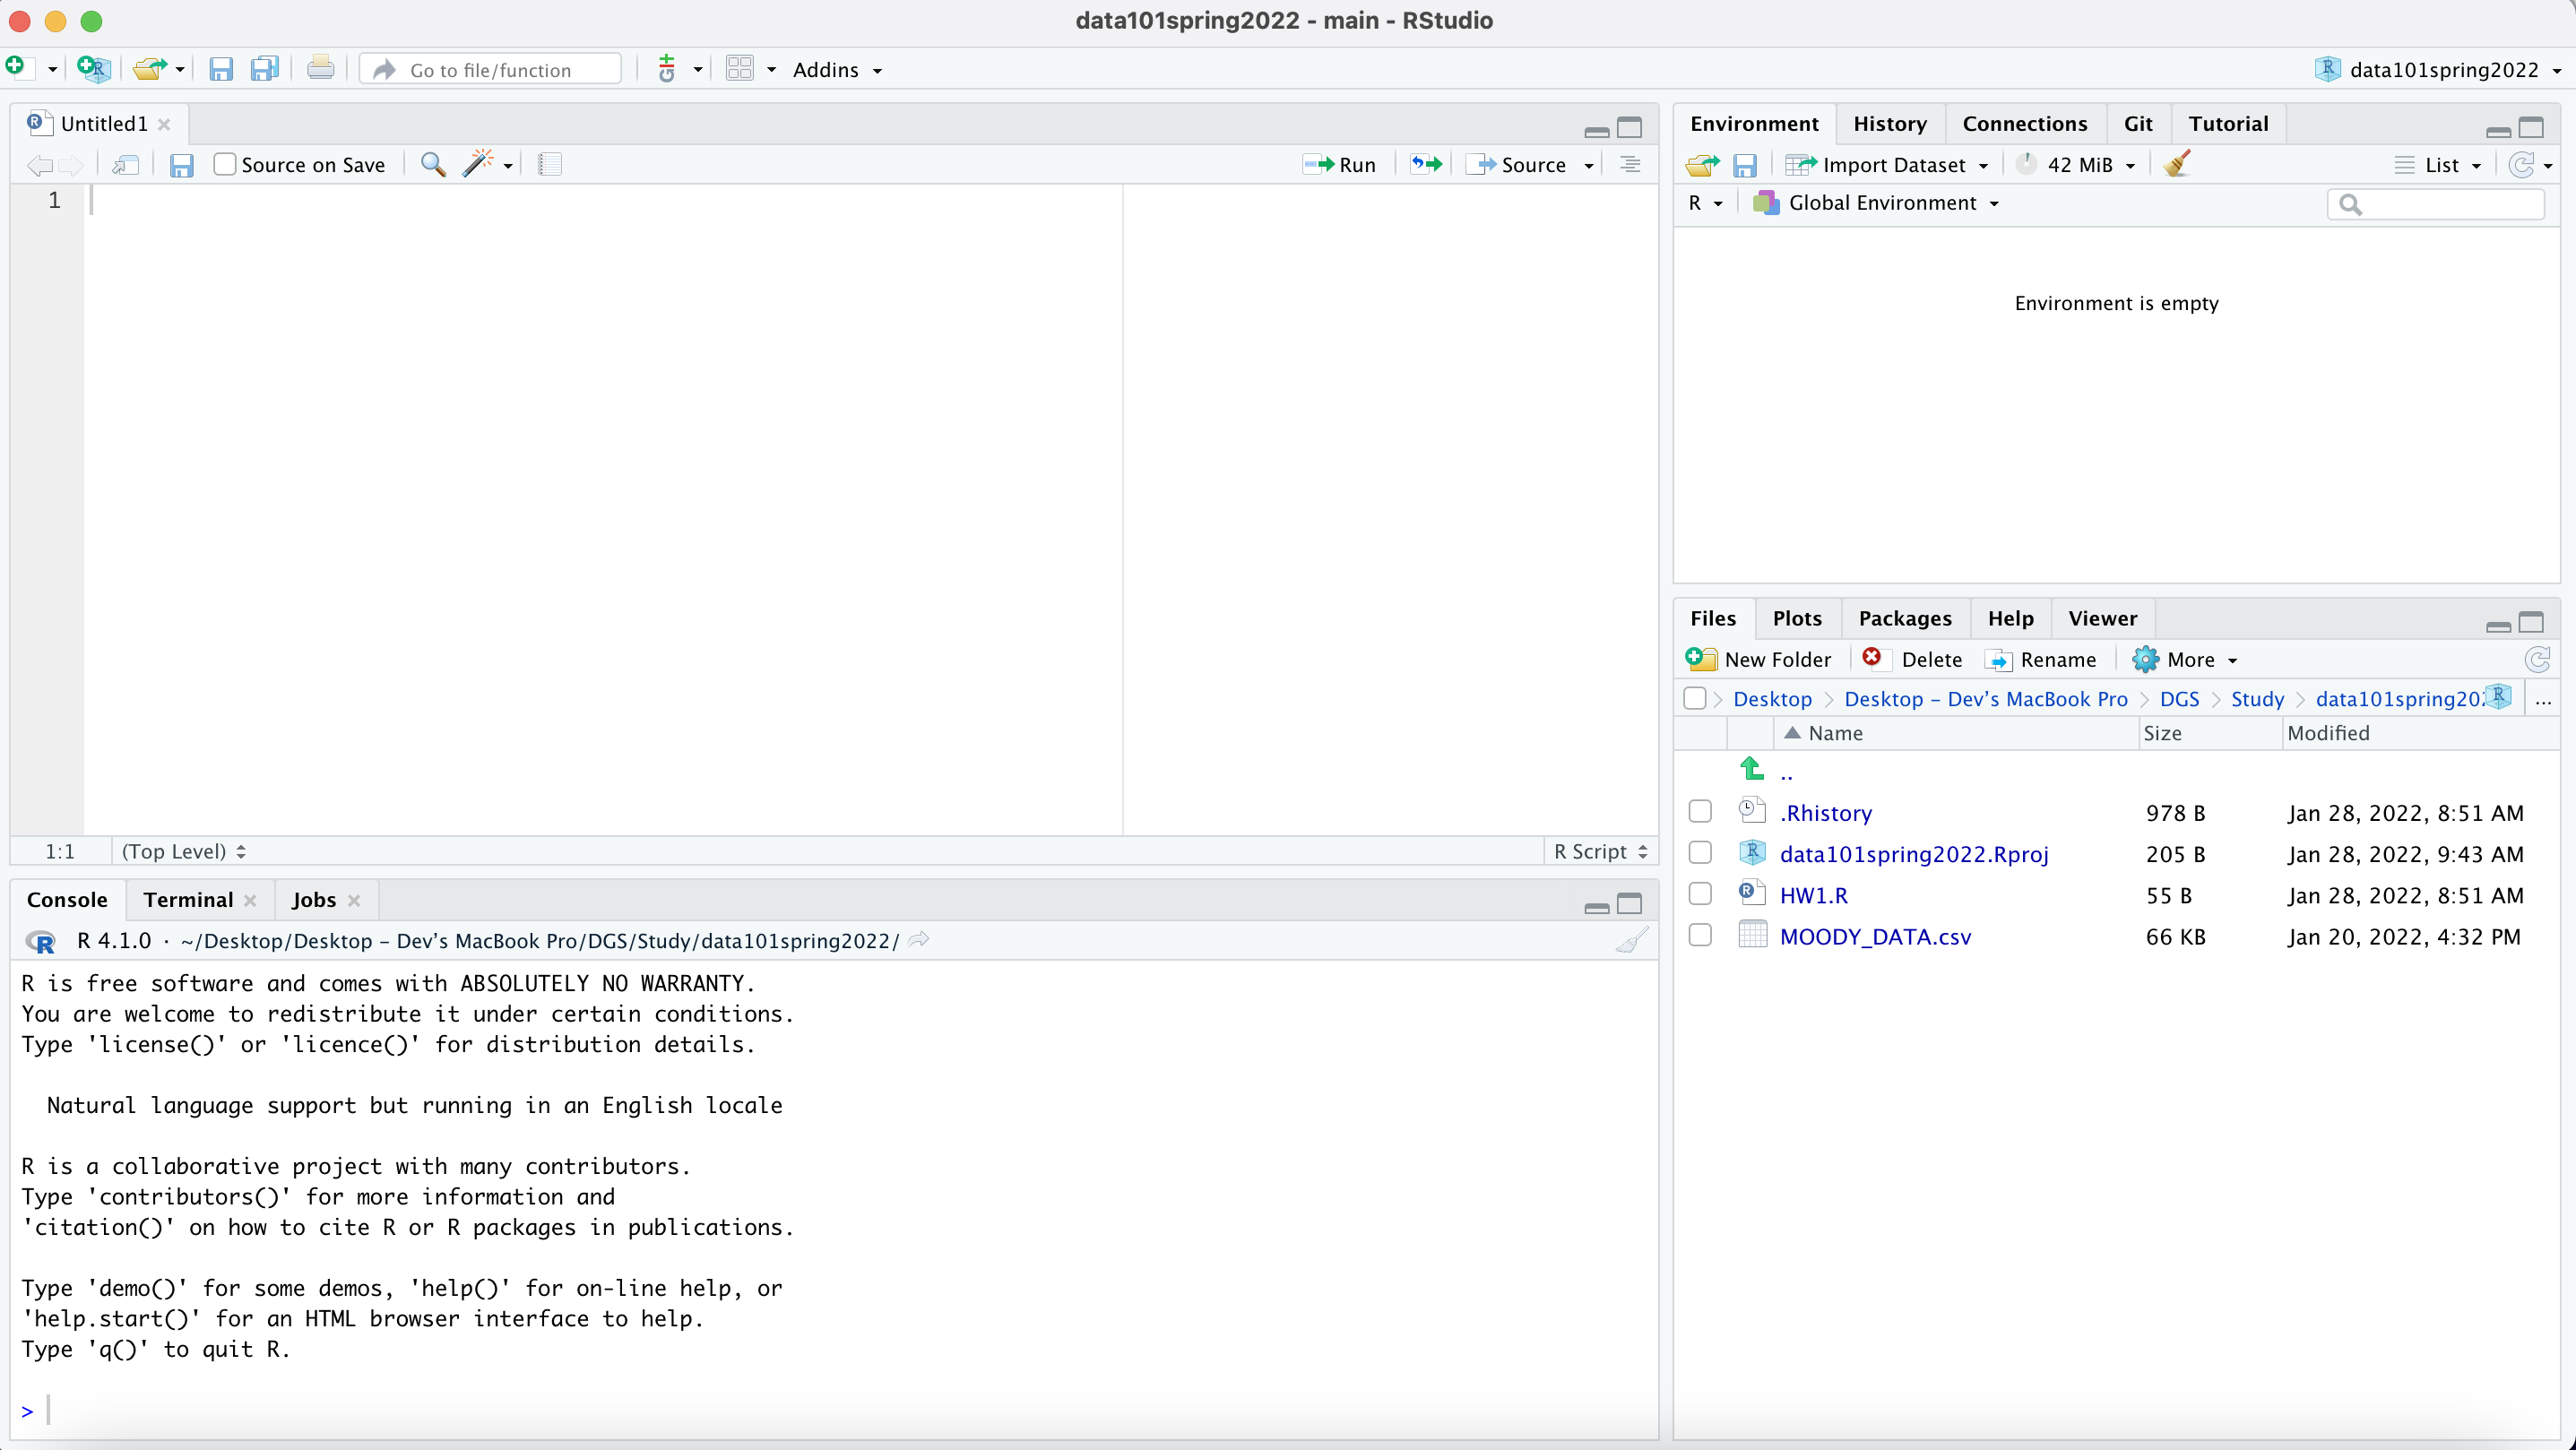
\includegraphics{https://raw.githubusercontent.com/dev7796/data101_tutorial/main/files/img/plots/4.5_text.png}
\caption{Rstudio}
\end{figure}

\begin{center}\rule{0.5\linewidth}{0.5pt}\end{center}

\hypertarget{how-to-upload-a-data-set}{%
\subsection{How to upload a data set?}\label{how-to-upload-a-data-set}}

\begin{itemize}
\item
  To upload the dataset/file present in csv format the read.csv() and read.csv2() functions are frequently used The read.csv() and read.csv2() have different separator symbol: for the former this is a comma, whereas the latter uses a semicolon.
\item
  There are two options while accessing the dataset from your local machine:

  \begin{enumerate}
  \def\labelenumi{\arabic{enumi}.}
  \tightlist
  \item
    To avoid giving long directory paths for accessing the dataset, one should use the command \textbf{getwd()} to get the current working directory and store the dataset in the same directory.
  \end{enumerate}
\end{itemize}

\begin{figure}
\centering
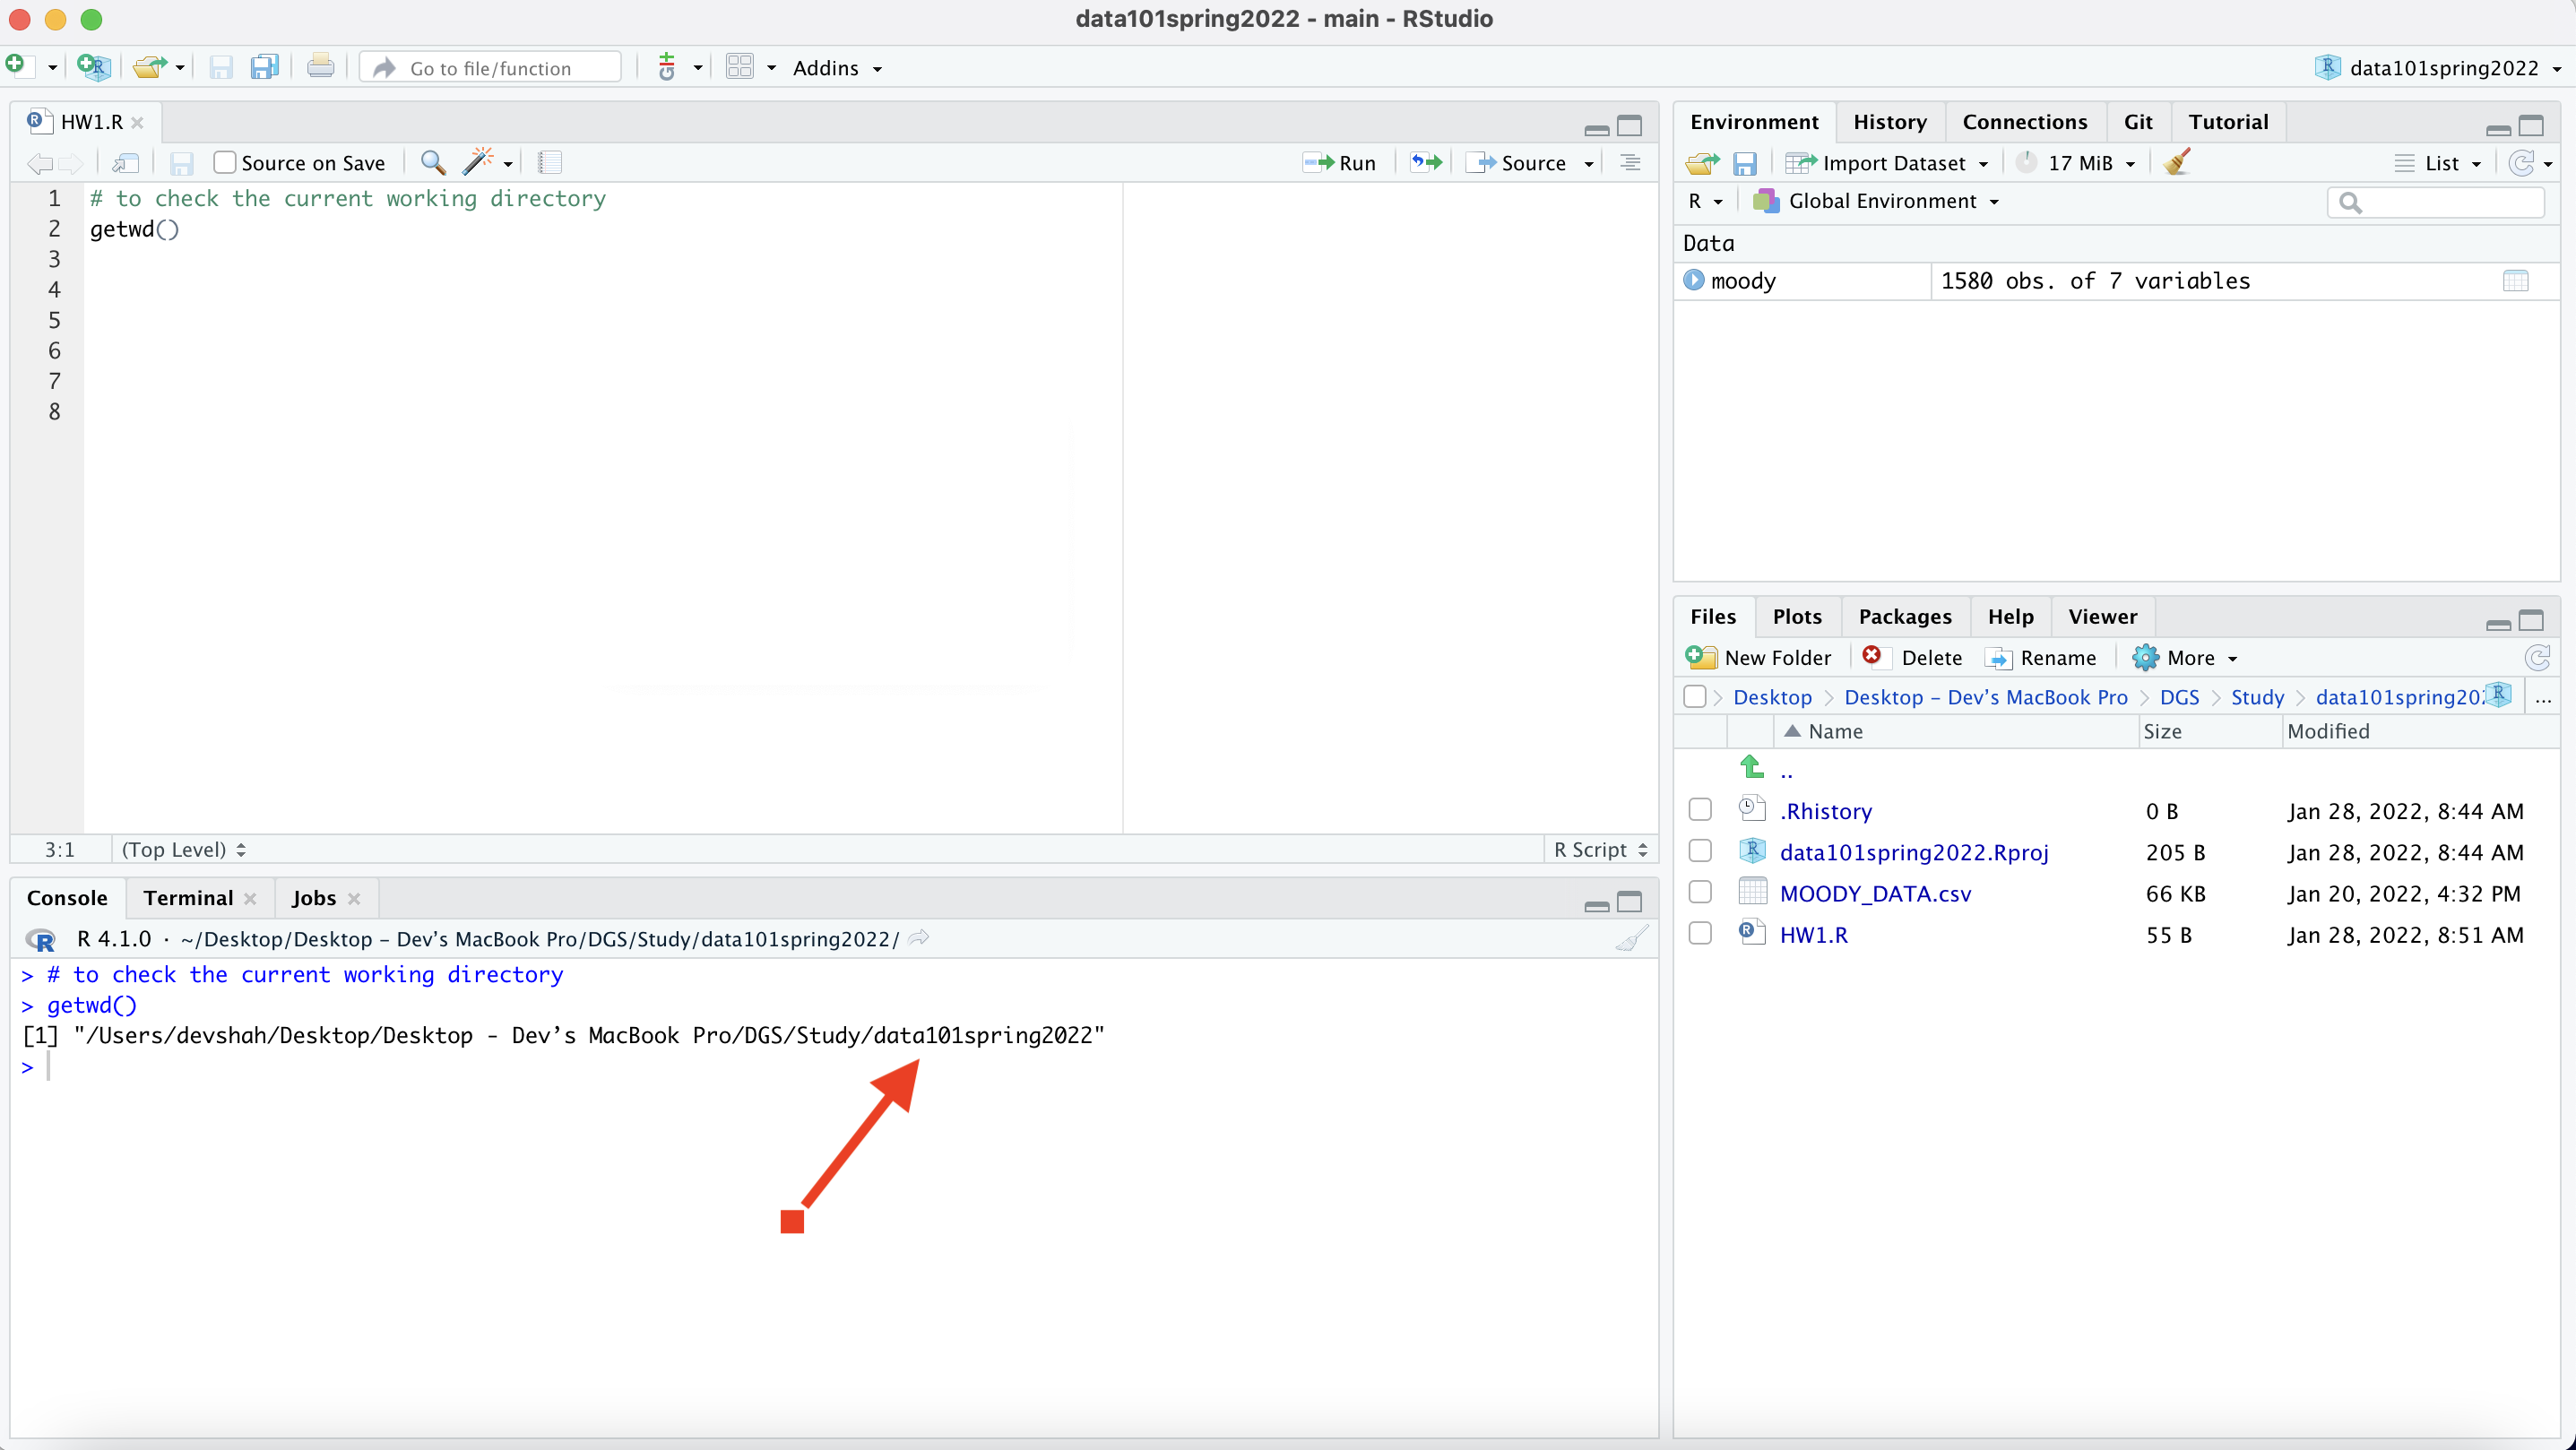
\includegraphics{https://raw.githubusercontent.com/dev7796/data101_tutorial/main/files/img/plots/5_text.png}
\caption{Getwd}
\end{figure}

\begin{itemize}
\tightlist
\item
  To access the dataset stored in the same directory one can use the following: \textbf{read.csv(``MOODY\_DATA.csv'')}.
\end{itemize}

\begin{figure}
\centering
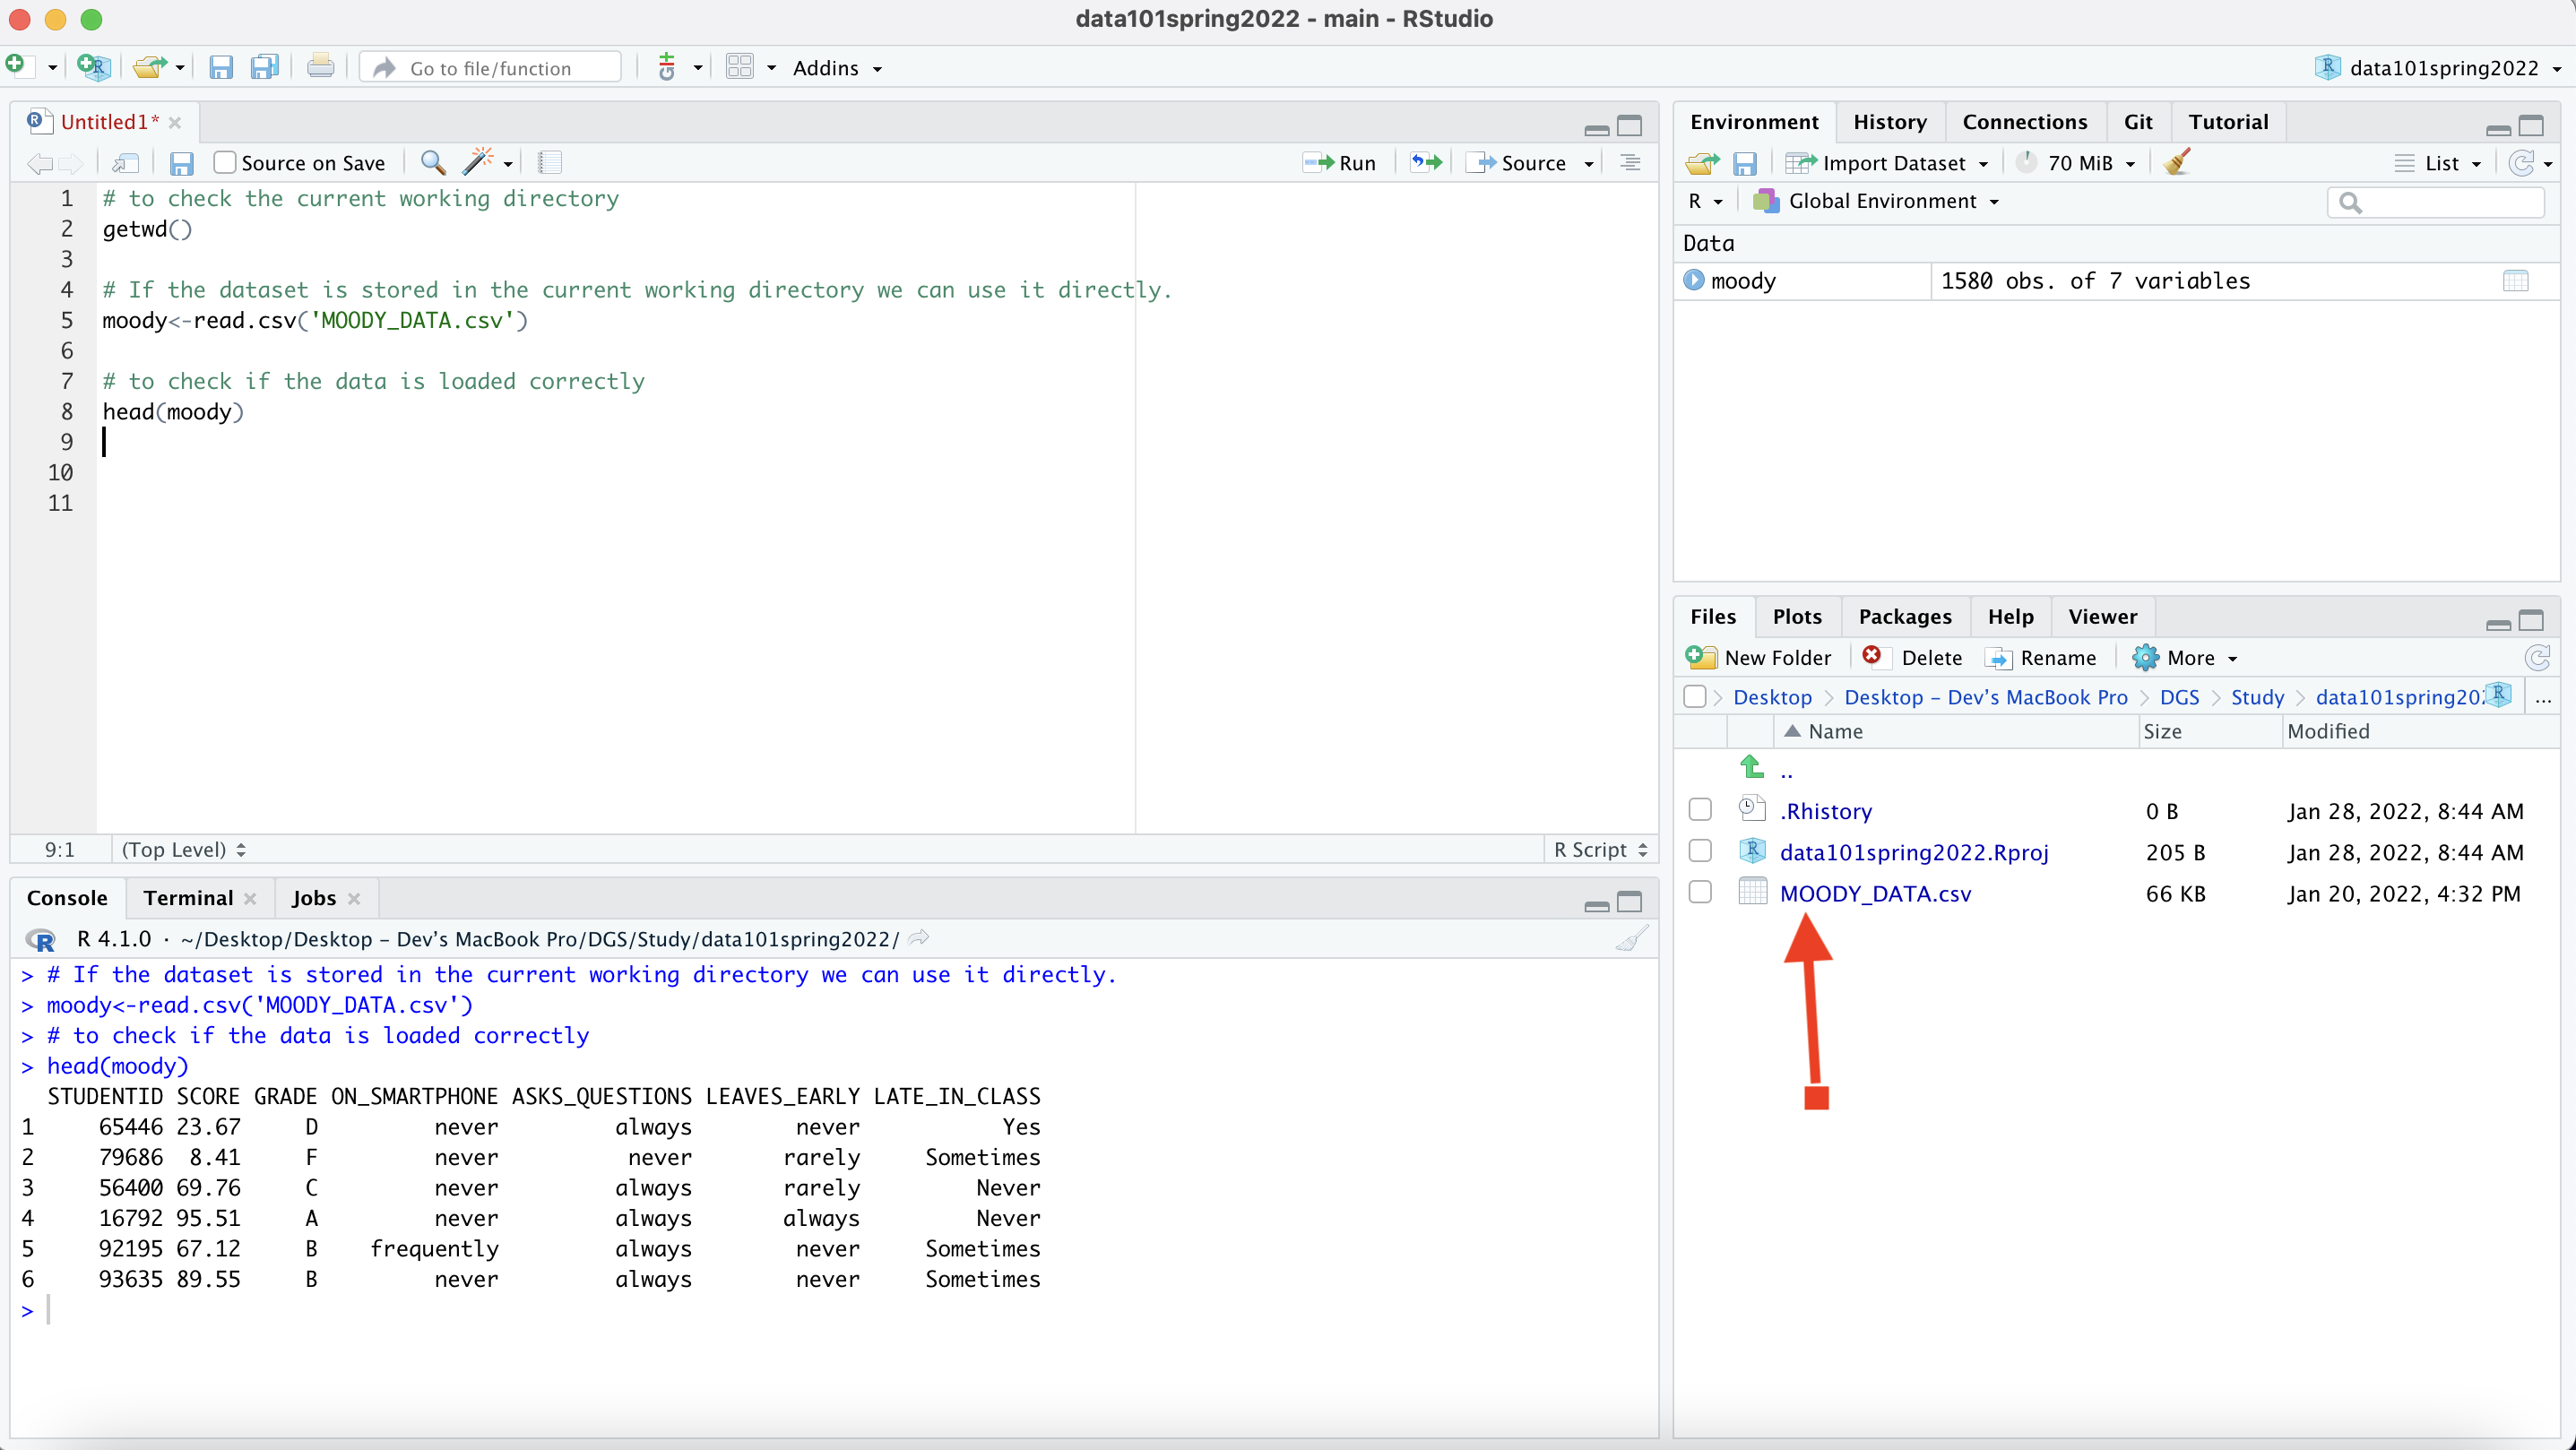
\includegraphics{https://raw.githubusercontent.com/dev7796/data101_tutorial/main/files/img/plots/6_text.png}
\caption{Store the moody dataset in the same directory}
\end{figure}

\begin{enumerate}
\def\labelenumi{\arabic{enumi}.}
\setcounter{enumi}{1}
\tightlist
\item
  One can also store the dataset at a different location and can access it using the following command: (Suppose the dataset is stored inside the folder Data101\_Tutorials on the desktop)
\end{enumerate}

\begin{verbatim}
- For Windows Users.
  - Example: read.csv("C:/Users/Desktop/Data101_Tutorials/MOODY_DATA.csv")

- For MAC Users.
  - Example: read.csv("/Users/Desktop/Data101_Tutorials/MOODY_DATA.csv")
  
\end{verbatim}

\textbf{Note: }
The directory path given here is the current working directory hosted on \emph{Github} where the dataset has been stored.

eyJsYW5ndWFnZSI6InIiLCJzYW1wbGUiOiIjIFJlYWQgaW4gdGhlIGRhdGFcbmRmIDwtIHJlYWQuY3N2KFwiaHR0cHM6Ly9yYXcuZ2l0aHVidXNlcmNvbnRlbnQuY29tL2Rldjc3OTYvZGF0YTEwMV90dXRvcmlhbC9tYWluL2ZpbGVzL2RhdGFzZXQvbW9vZHkyMDIwYi5jc3ZcIilcblxuIyBQcmludCBvdXQgYGRmYFxuaGVhZChkZikifQ==

\begin{center}\rule{0.5\linewidth}{0.5pt}\end{center}

\hypertarget{saving-your-work}{%
\subsection{Saving your work}\label{saving-your-work}}

\begin{itemize}
\tightlist
\item
  To save your work go to \textbf{File -\textgreater{} Save}. It will ask you to give a name for your \textbf{.R file} and then click on Save.
\end{itemize}

\begin{figure}
\centering
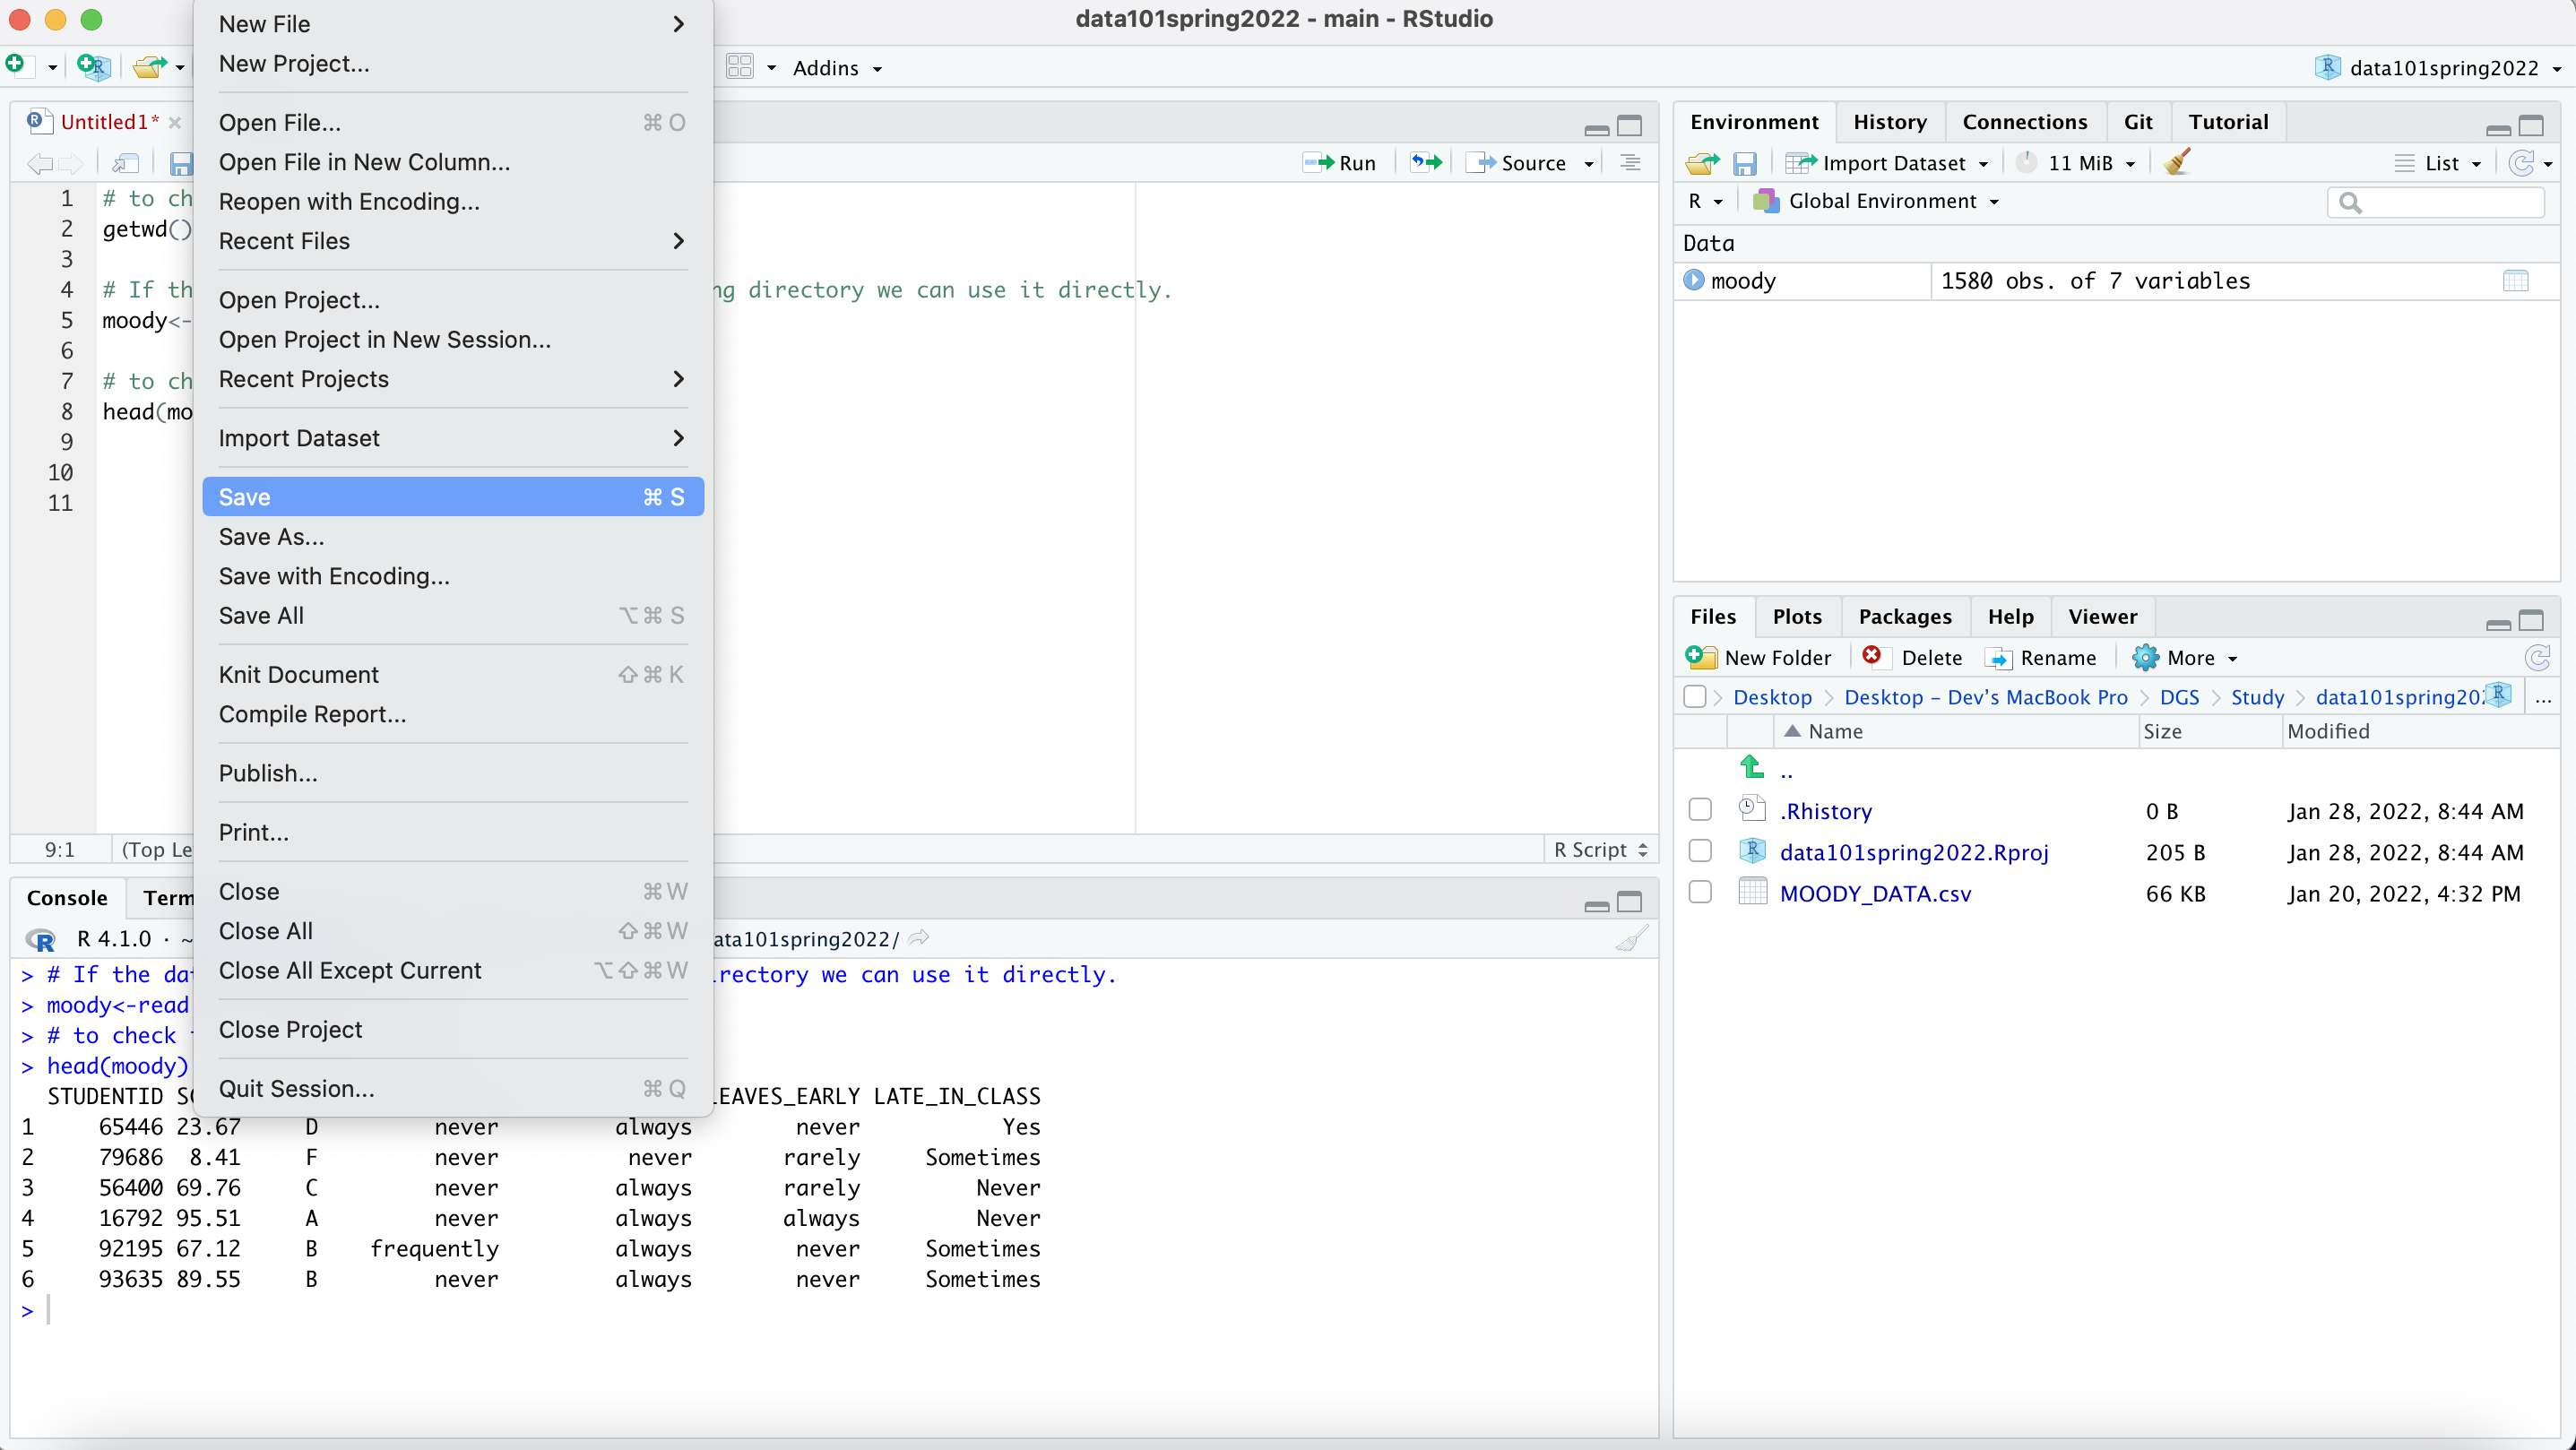
\includegraphics{https://raw.githubusercontent.com/dev7796/data101_tutorial/main/files/img/plots/7_text.png}
\caption{Save}
\end{figure}

\begin{itemize}
\tightlist
\item
  After making modifications to your saved file, you will need to save the file again.
  If the name of the file on the top is in { Red Color } indicates that the file have \textbf{unsaved} changes.
\end{itemize}

\begin{figure}
\centering
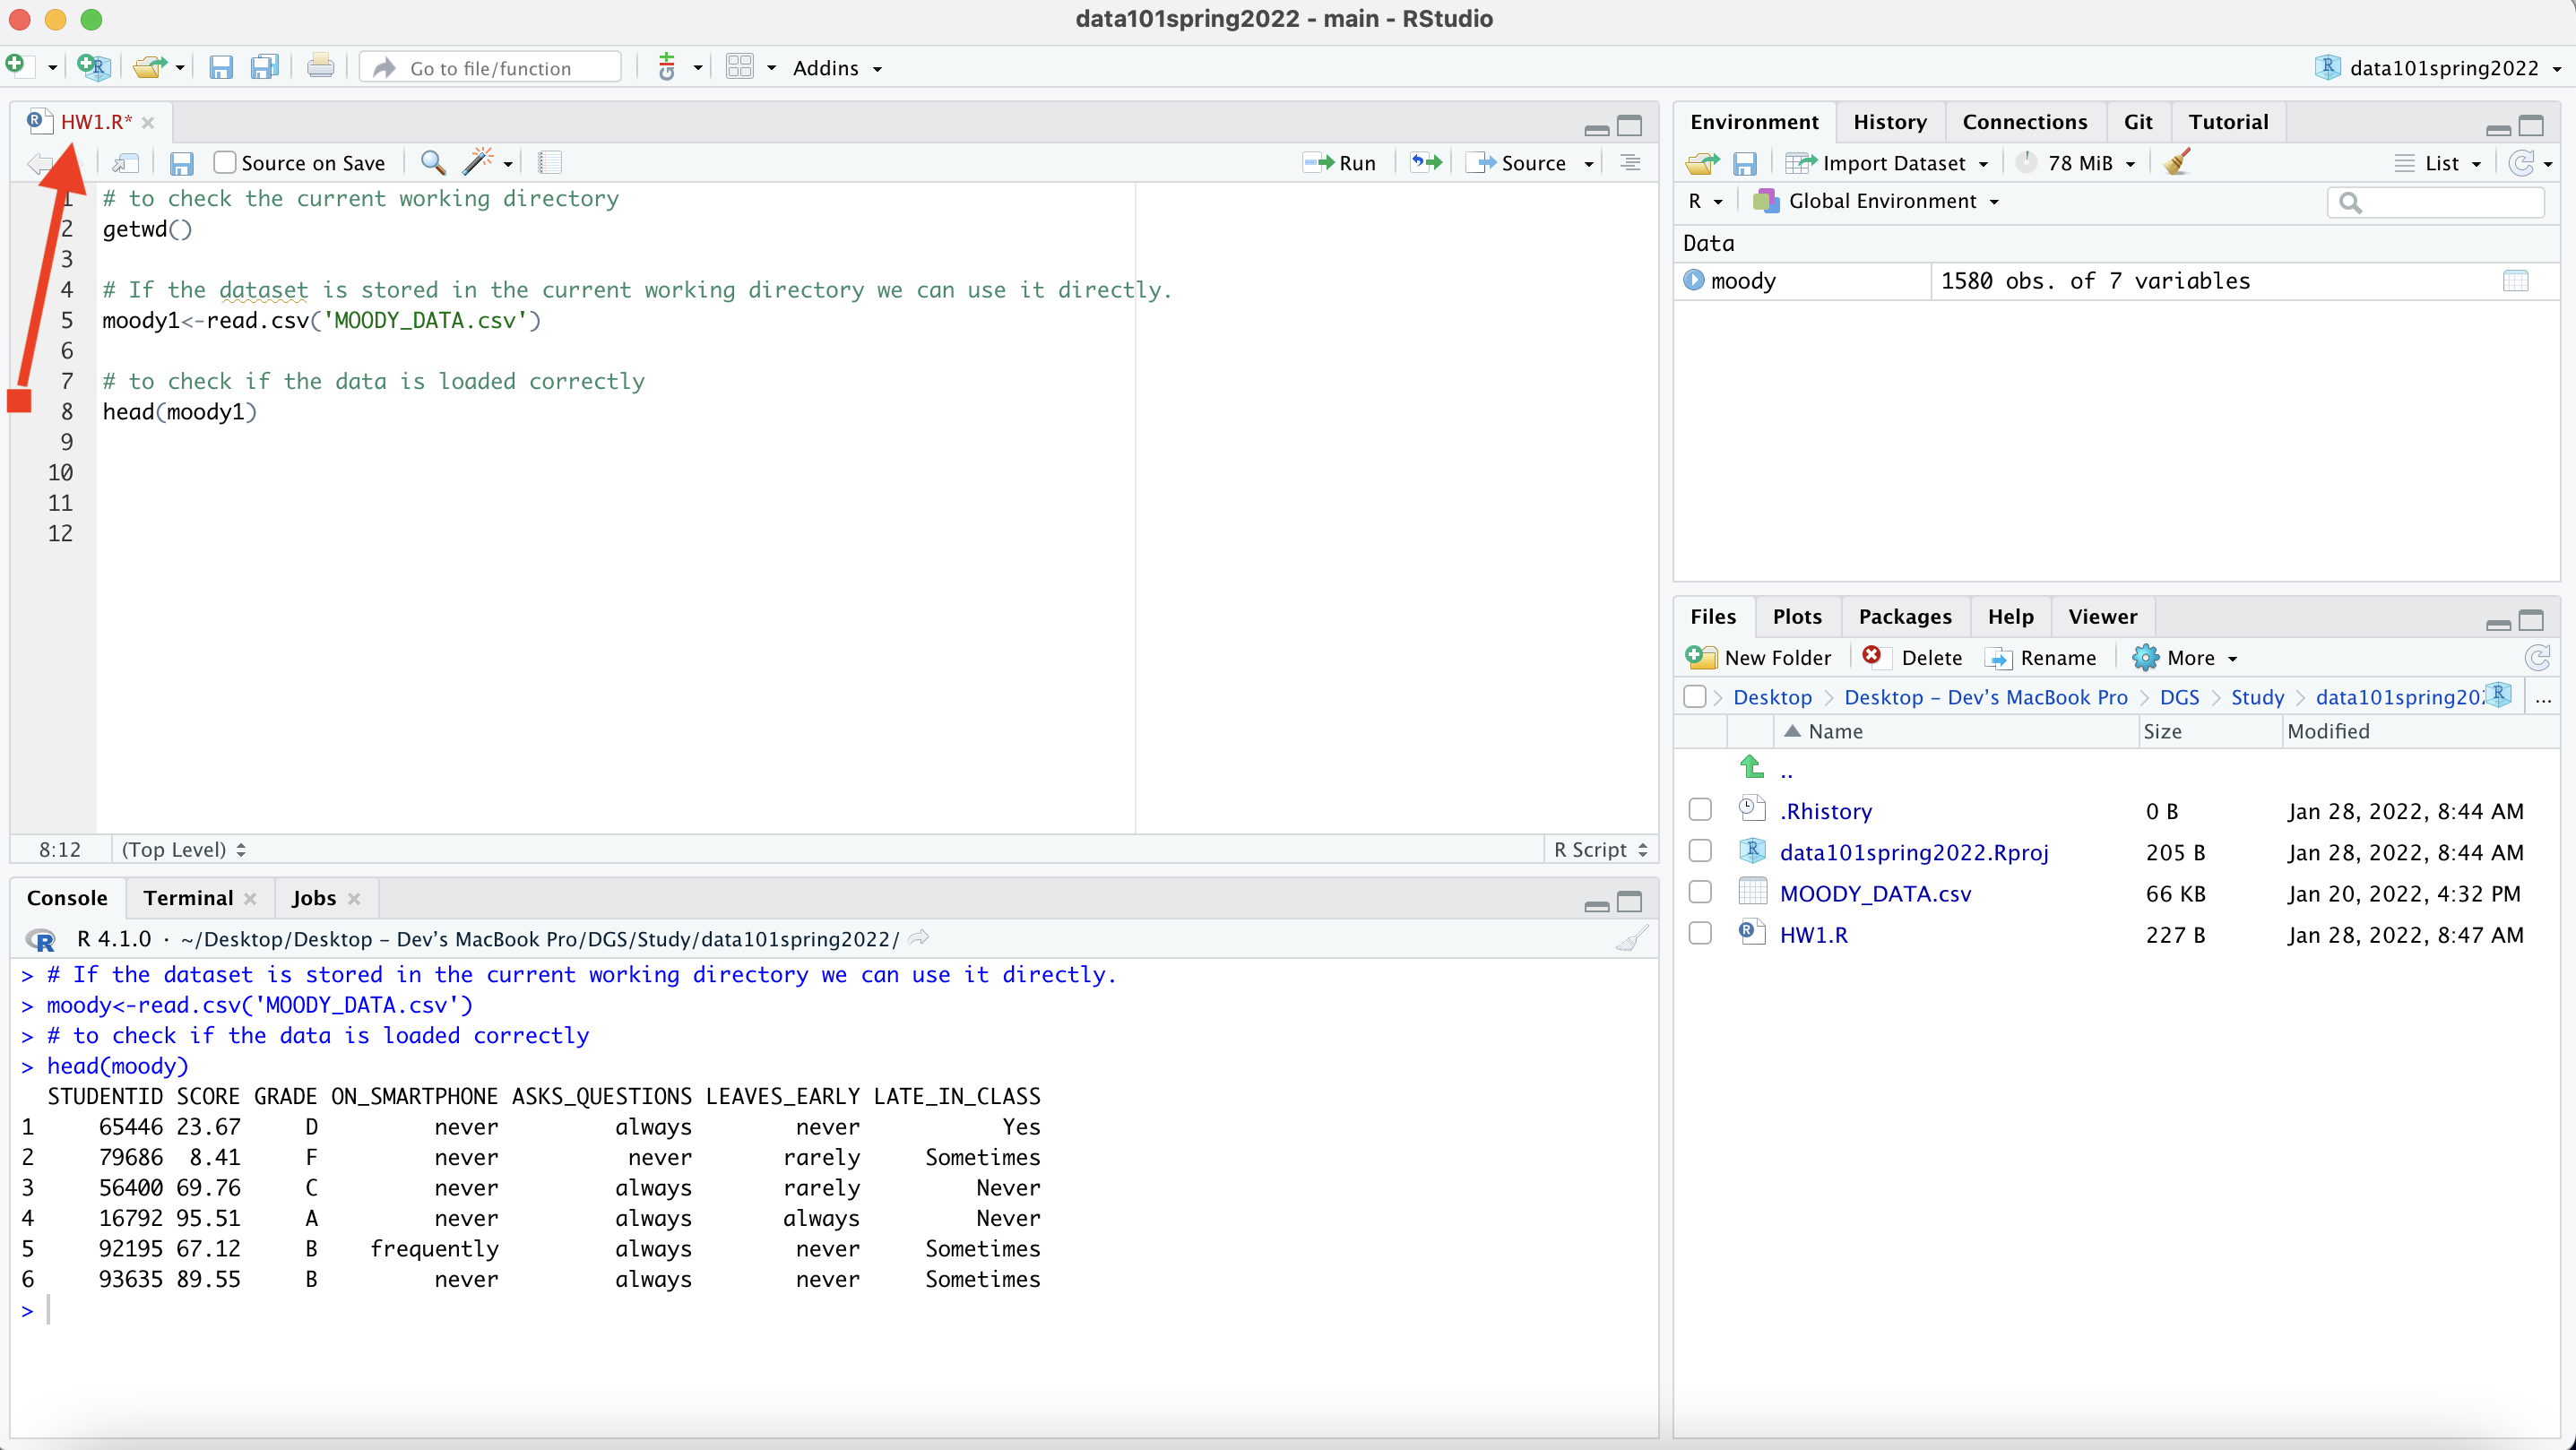
\includegraphics{https://raw.githubusercontent.com/dev7796/data101_tutorial/main/files/img/plots/8_text.png}
\caption{Unsaved File}
\end{figure}

\begin{itemize}
\tightlist
\item
  Go to \textbf{File -\textgreater{} Save} to save your .R file again. After saving the file the color of the file name i.e.~\textbf{HW1.R} will again change back to \textbf{black}.
\end{itemize}

\begin{figure}
\centering
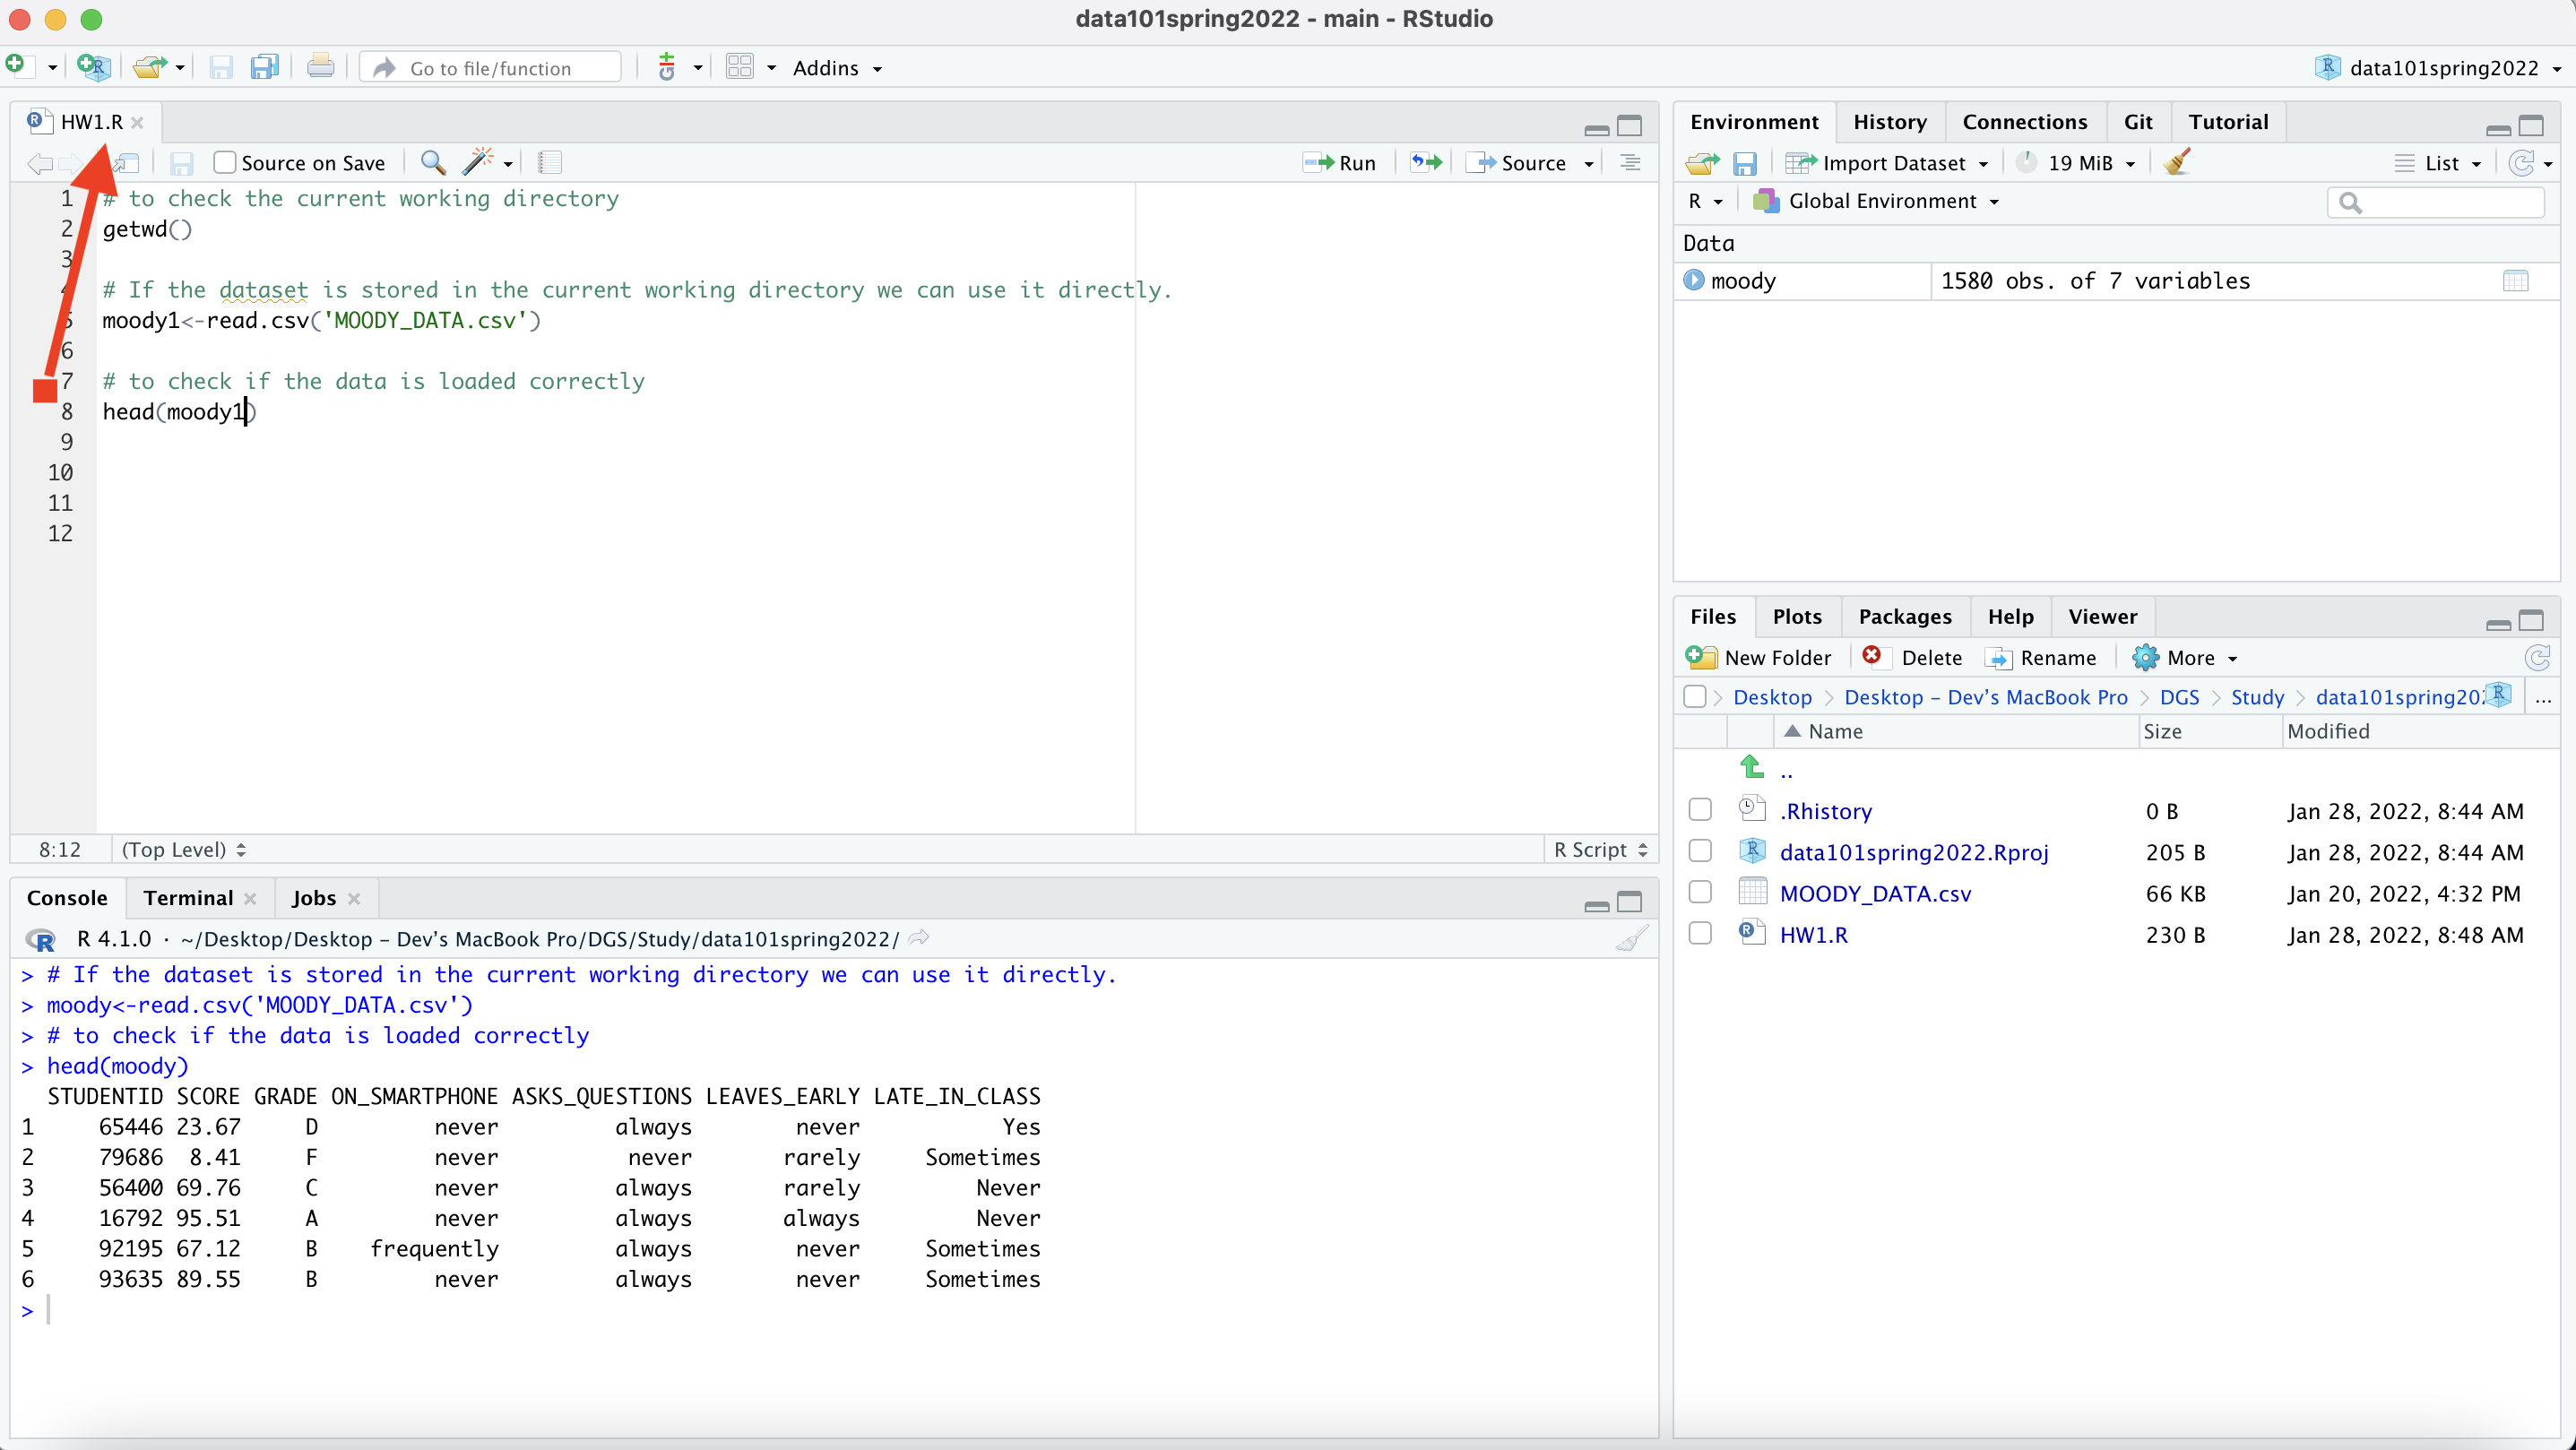
\includegraphics{https://raw.githubusercontent.com/dev7796/data101_tutorial/main/files/img/plots/9_text.png}
\caption{Saved File}
\end{figure}

\textbf{Note: } You can create multiple files inside the same project such as for your each homework assignments

\hypertarget{general-r-references}{%
\subsection{General R References}\label{general-r-references}}

\url{https://www.w3schools.com/r/}
\url{https://cran.r-project.org/doc/contrib/Short-refcard.pdf}
\url{https://www.amazon.com/Statistics-Engineers-Scientists-William-Navidi/dp/0073376337/ref=pd_lpo_3?pd_rd_i=0073376337\&psc=1}

\hypertarget{textbook-concepts}{%
\subsection{Textbook Concepts}\label{textbook-concepts}}

\begin{itemize}
\item
  Hypothesis testing: \ref{ztest}, \ref{ptest}
\item
  Difference of means hypothesis testing: \ref{ptest}
\item
  Null Hypothesis: \ref{ztest}
\item
  Alternative Hypothesis: \ref{ztest}
\item
  z-value: \ref{ztest}
\item
  critical value: \ref{ztest}
\item
  significance level: \ref{ztest}
\item
  p-value: \ref{ztest}
\item
  Bonferroni correction: \ref{Mtest}
\item
  Chi square test: \ref{chitest}
\item
  Independence: \ref{chitest}
\item
  Multiple Hypothesis testing: \ref{Mtest}
\item
  False Discovery Proportion: \ref{Mtest}
\item
  Contingency Matrix: \ref{chitest}
\item
  Bayesian Reasoning: \ref{br}
\item
  Prior odds: \ref{br}
\item
  Posterior odds: \ref{br}
\item
  Likelihood ratio: \ref{br}
\item
  False positive: \ref{br}
\item
  True positive: \ref{br}
\item
  Crossvalidation: \ref{crossvalidation}
\item
  Decision trees: \ref{prpart}
\item
  Linear regression: \ref{lr}
\item
  Recursive partitioning: \ref{lr}
\item
  MSE: \ref{lr}
\item
  Prediction accuracy: \ref{lr}
\item
  Training: \ref{lr}
\item
  Testing: \ref{lr}
\end{itemize}

\hypertarget{r-functions-used-in-this-class}{%
\subsection{R functions used in this class}\label{r-functions-used-in-this-class}}

\begin{itemize}
\item
  \textbf{Elementary instructions: } c() \ref{vector}, mean() \ref{mean}, nrow() \ref{nrow}, rep(), sd() \ref{sd}, cut() \ref{cut}
\item
  \textbf{Plots: } plot() \ref{scartterplot}, barplot() \ref{barplot}, boxplot() \ref{boxplot} mosaicplot() \ref{mosaicplot}
\item
  \textbf{Data Transformations: } subset() \ref{subset}, tapply() \ref{tapply}, table() \ref{table}, aggregate()
\item
  \textbf{Library functions: } chisq.test() \ref{chitest}, pnorm() \ref{pnorm}, Permutation() \ref{ptest}, rpart() \ref{prpart}, predict() \ref{rpartpredict}, lm() \ref{lm}, crossvalidation() \ref{crossvalidation}
\item
  \textbf{Parameters of rpart: } minsplit \ref{rpartcontrol}, minbucket \ref{rpartcontrol}, cp \ref{rpartcontrol}
\end{itemize}

\hypertarget{data-sets}{%
\subsection{Data sets}\label{data-sets}}

\hypertarget{moody}{%
\subsubsection{Moody}\label{moody}}

\begin{table}

\caption{\label{tab:unnamed-chunk-26}Snippet of Moody Dataset}
\centering
\begin{tabular}[t]{lrlllr}
\toprule
  & SCORE & GRADE & DOZES\_OFF & TEXTING\_IN\_CLASS & PARTICIPATION\\
\midrule
393 & 67.93 & C & always & never & 0.09\\
127 & 57.10 & C & sometimes & never & 0.48\\
717 & 25.02 & D & always & never & 0.02\\
573 & 61.82 & B & sometimes & rarely & 0.00\\
318 & 98.28 & A & always & never & 0.99\\
\bottomrule
\end{tabular}
\end{table}

eyJsYW5ndWFnZSI6InIiLCJzYW1wbGUiOiJtb29keTwtcmVhZC5jc3YoXCJodHRwczovL3Jhdy5naXRodWJ1c2VyY29udGVudC5jb20vZGV2Nzc5Ni9kYXRhMTAxX3R1dG9yaWFsL21haW4vZmlsZXMvZGF0YXNldC9tb29keTIwMjJfbmV3LmNzdlwiKVxuXG5zdW1tYXJ5KG1vb2R5KSJ9

\hypertarget{movies}{%
\subsubsection{Movies}\label{movies}}

\begin{table}

\caption{\label{tab:unnamed-chunk-28}Snippet of Movies Dataset}
\centering
\begin{tabular}[t]{lllrlll}
\toprule
  & country & content & imdb\_score & Gross & Budget & genre\\
\midrule
11322 & USA & PG-13 & 8.11 & Low & Low & History\\
11045 & USA & PG & 8.20 & Medium & Low & Drama\\
8995 & USA & PG & 6.86 & Medium & Low & History\\
2657 & USA & R & 5.63 & Medium & High & Family\\
9762 & USA & R & 7.79 & Medium & Low & History\\
\bottomrule
\end{tabular}
\end{table}

eyJsYW5ndWFnZSI6InIiLCJzYW1wbGUiOiJtb3ZpZXM8LXJlYWQuY3N2KFwiaHR0cHM6Ly9yYXcuZ2l0aHVidXNlcmNvbnRlbnQuY29tL2Rldjc3OTYvZGF0YTEwMV90dXRvcmlhbC9tYWluL2ZpbGVzL2RhdGFzZXQvTW92aWVzMjAyMkYtNC5jc3ZcIilcblxuc3VtbWFyeShtb3ZpZXMpIn0=

\hypertarget{traffic}{%
\subsubsection{Traffic}\label{traffic}}

\begin{table}

\caption{\label{tab:unnamed-chunk-30}Snippet of Traffic Dataset}
\centering
\begin{tabular}[t]{lllr}
\toprule
  & TUNNEL & DAY & VOLUME\_PER\_MINUTE\\
\midrule
1854 & Lincoln & weekday & 100.0\\
1793 & Lincoln & weekday & 83.0\\
270 & Holland & weekday & 58.5\\
1928 & Lincoln & weekday & 68.0\\
95 & Holland & weekday & 36.5\\
\bottomrule
\end{tabular}
\end{table}

eyJsYW5ndWFnZSI6InIiLCJzYW1wbGUiOiJ0cmFmZmljPC1yZWFkLmNzdignaHR0cHM6Ly9yYXcuZ2l0aHVidXNlcmNvbnRlbnQuY29tL2Rldjc3OTYvZGF0YTEwMV90dXRvcmlhbC9tYWluL2ZpbGVzL2RhdGFzZXQvVHJhZmZpYzIwMjIuY3N2Jylcblxuc3VtbWFyeSh0cmFmZmljKSJ9

\hypertarget{hindex}{%
\subsubsection{Hindex}\label{hindex}}

\begin{table}

\caption{\label{tab:unnamed-chunk-32}Snippet of Hindex Dataset}
\centering
\begin{tabular}[t]{lrlr}
\toprule
  & IDN & COUNTRY & HAPPINESS\\
\midrule
5746 & 76397 & Georgia & 7.72\\
2837 & 19119 & Sierra Leone & 2.21\\
4640 & 97602 & Jordan & 9.41\\
3523 & 65736 & Kenya & 6.70\\
4853 & 94589 & Azerbaijan & 9.40\\
\bottomrule
\end{tabular}
\end{table}

eyJsYW5ndWFnZSI6InIiLCJzYW1wbGUiOiJoaW5kZXggPC1yZWFkLmNzdihcImh0dHBzOi8vcmF3LmdpdGh1YnVzZXJjb250ZW50LmNvbS9kZXY3Nzk2L2RhdGExMDFfdHV0b3JpYWwvbWFpbi9maWxlcy9kYXRhc2V0L0hpbmRleC5jc3ZcIilcblxuc3VtbWFyeShoaW5kZXgpIn0=

\hypertarget{prediction-1-dataset}{%
\subsubsection{Prediction 1 Dataset}\label{prediction-1-dataset}}

\begin{table}

\caption{\label{tab:unnamed-chunk-34}Snippet of Moody Predicition 1 dataset}
\centering
\begin{tabular}[t]{llrll}
\toprule
  & Major & Score & Seniority & Grade\\
\midrule
209 & CS & 83 & Freshman & A\\
674 & CS & 44 & Senior & F\\
203 & Economics & 35 & Junior & F\\
69 & Statistics & 93 & Senior & A\\
339 & Statistics & 81 & Sophomore & B\\
\bottomrule
\end{tabular}
\end{table}

eyJsYW5ndWFnZSI6InIiLCJzYW1wbGUiOiJtb29keTwtcmVhZC5jc3YoXCJodHRwczovL3Jhdy5naXRodWJ1c2VyY29udGVudC5jb20vZGV2Nzc5Ni9kYXRhMTAxX3R1dG9yaWFsL21haW4vZmlsZXMvZGF0YXNldC9NMjAyMnRyYWluLmNzdlwiKVxuXG5zdW1tYXJ5KG1vb2R5KSJ9

\hypertarget{midterm-project-and-final-exam-distribution-in-prof.-moody-class}{%
\subsubsection{Midterm, Project and Final Exam distribution in Prof.~Moody class}\label{midterm-project-and-final-exam-distribution-in-prof.-moody-class}}

\textbf{Assumptions:} Midterm, Project and Final Exam are all out of 100

\begin{table}

\caption{\label{tab:unnamed-chunk-36}Midterm, Project and Final Exam distribution in Prof. Moody class}
\centering
\begin{tabular}[t]{lrrrr}
\toprule
  & Midterm & Project & FinalExam & ClassScore\\
\midrule
845 & 10 & 99 & 9 & 54.20000\\
809 & 26 & 16 & 76 & 36.20084\\
431 & 33 & 24 & 50 & 33.60000\\
5 & 85 & 52 & 85 & 68.50000\\
849 & 22 & 32 & 2 & 21.00000\\
\bottomrule
\end{tabular}
\end{table}

eyJsYW5ndWFnZSI6InIiLCJzYW1wbGUiOiJtb29keTwtcmVhZC5jc3YoXCJodHRwczovL3Jhdy5naXRodWJ1c2VyY29udGVudC5jb20vZGV2Nzc5Ni9kYXRhMTAxX3R1dG9yaWFsL21haW4vZmlsZXMvZGF0YXNldC9Nb29keU5VTS5jc3ZcIilcblxuc3VtbWFyeShtb29keSkifQ==

\hypertarget{minimarket}{%
\subsubsection{Minimarket}\label{minimarket}}

\begin{table}

\caption{\label{tab:unnamed-chunk-38}Minimarket dataset}
\centering
\begin{tabular}[t]{llllllll}
\toprule
  & Beer & Day & Location & SoftDrinks & Sweets & Wine & Snacks\\
\midrule
7908 & Ale & Weekend & Edison & Orange  Juice & Milky Way & Red & None\\
3699 & Lager & Weekday & New Brunswick & Sprite & Snickers & None & Pretzels\\
11944 & Ale & Weekday & Edison & Orange  Juice & Snickers & None & None\\
10944 & Lager & Weekday & Princeton & Orange  Juice & Snickers & None & Popcorn\\
15790 & Lager & Weekday & Edison & Sprite & Milky Way & White & Popcorn\\
\bottomrule
\end{tabular}
\end{table}

eyJsYW5ndWFnZSI6InIiLCJzYW1wbGUiOiJtaW5pbWFya2V0PC1yZWFkLmNzdihcImh0dHBzOi8vcmF3LmdpdGh1YnVzZXJjb250ZW50LmNvbS9kZXY3Nzk2L2RhdGExMDFfdHV0b3JpYWwvbWFpbi9maWxlcy9kYXRhc2V0L0hvbWV3b3JrTWFya2V0MjAyMi5jc3ZcIilcblxuc3VtbWFyeShtaW5pbWFya2V0KSJ9

\hypertarget{plots}{%
\section{🔖 Plots}\label{plots}}

\begin{itemize}
\tightlist
\item
  \textbf{Lecture slides: } Plots

  \hypertarget{plots12}{}
\end{itemize}

\hypertarget{vector}{%
\subsection{Vector}\label{vector}}

\begin{itemize}
\tightlist
\item
  A vector is simply a list of items that are of the same type.
\end{itemize}

\hypertarget{snippet-1}{%
\subsubsection{Snippet 1}\label{snippet-1}}

Lets look at example of creating a vector:

eyJsYW5ndWFnZSI6InIiLCJzYW1wbGUiOiIjTGV0cyBjcmVhdGUgMyB2ZWN0b3JzIHdpdGggdGl0bGUsIGF1dGhvciBhbmQgeWVhci5cbmNvbG9yIDwtIGMoJ1JlZCcsJ0JsdWUnLCdZZWxsb3cnLCdHcmVlbicpXG5cbiNMZXRzIGxvb2sgYXQgaG93IHRoZSBjcmVhdGVkIHZlY3RvcnMgbG9vay5cbmNvbG9yIn0=

\hypertarget{snippet-2}{%
\subsubsection{Snippet 2}\label{snippet-2}}

Create a vector with numerical values in a sequence, use the \textbf{:} operator:

eyJsYW5ndWFnZSI6InIiLCJzYW1wbGUiOiIjTGV0cyBjcmVhdGUgYSB2ZWN0b3JzIHdpdGggbnVtZXJpY2FsIHNlcXVlbmNlLlxueWVhciA8LSAyMDE4OjIwMjJcblxuI0xldHMgbG9vayBhdCBob3cgdGhlIGNyZWF0ZWQgdmVjdG9ycyBsb29rLlxueWVhciJ9

\begin{center}\rule{0.5\linewidth}{0.5pt}\end{center}

\hypertarget{data-frames}{%
\subsection{Data Frames}\label{data-frames}}

\begin{itemize}
\tightlist
\item
  Data Frames are data displayed in a format as a table.
\end{itemize}

\hypertarget{snippet-1-1}{%
\subsubsection{Snippet 1}\label{snippet-1-1}}

Populating the dataframe:

eyJsYW5ndWFnZSI6InIiLCJzYW1wbGUiOiIjIExvYWQgdGhlIGRhdGFzZXQgaW50byB0aGUgbW9vZHkgdmFyaWFibGVcbm1vb2R5PC1yZWFkLmNzdihcImh0dHBzOi8vcmF3LmdpdGh1YnVzZXJjb250ZW50LmNvbS9kZXY3Nzk2L2RhdGExMDFfdHV0b3JpYWwvbWFpbi9maWxlcy9kYXRhc2V0L21vb2R5MjAyMGIuY3N2XCIpXG5cbiMgTm93IGxldHMgdmlldyB0aGUgZGF0YWZyYW1lIG1vb2R5IHdpdGgganVzdCA1LTYgdHVwbGVzXG5oZWFkKG1vb2R5KSJ9

\hypertarget{snippet-2-1}{%
\subsubsection{Snippet 2}\label{snippet-2-1}}

Get the summary of the dataframe:

eyJsYW5ndWFnZSI6InIiLCJzYW1wbGUiOiIjIExvYWQgdGhlIGRhdGFzZXQgaW50byB0aGUgbW9vZHkgdmFyaWFibGVcbm1vb2R5PC1yZWFkLmNzdihcImh0dHBzOi8vcmF3LmdpdGh1YnVzZXJjb250ZW50LmNvbS9kZXY3Nzk2L2RhdGExMDFfdHV0b3JpYWwvbWFpbi9maWxlcy9kYXRhc2V0L21vb2R5MjAyMGIuY3N2XCIpXG5cbiMgVXNlIHRoZSBzdW1tYXJ5KCkgZnVuY3Rpb24gdG8gc3VtbWFyaXplIHRoZSBkYXRhIGZyb20gYSBEYXRhIEZyYW1lOlxuc3VtbWFyeShtb29keSkifQ==

\hypertarget{snippet-3}{%
\subsubsection{Snippet 3}\label{snippet-3}}

Use the notation \textbf{data{[}rows, columns{]}}, which selects the subsets of rows and columns:

eyJsYW5ndWFnZSI6InIiLCJzYW1wbGUiOiIjIExvYWQgdGhlIGRhdGFzZXQgaW50byB0aGUgbW9vZHkgdmFyaWFibGVcbm1vb2R5PC1yZWFkLmNzdihcImh0dHBzOi8vcmF3LmdpdGh1YnVzZXJjb250ZW50LmNvbS9kZXY3Nzk2L2RhdGExMDFfdHV0b3JpYWwvbWFpbi9maWxlcy9kYXRhc2V0L21vb2R5MjAyMGIuY3N2XCIpXG5cbiMgUmV0dXJuIHJvdyAxXG5tb29keVsxLCBdXG5cbiMgUmV0dXJuIGNvbHVtbiA1XG5tb29keVssIDVdXG5cbiMgUm93cyAxOjUgYW5kIGNvbHVtbiAyXG5tb29keVsxOjUsIDJdXG5cbiMgR2l2ZSBtZSByb3dzIDEtMyBhbmQgY29sdW1ucyAyIGFuZCA0IG9mIG1vb2R5XG5tb29keVsxOjMsIGMoMjo0KV0ifQ==

\begin{center}\rule{0.5\linewidth}{0.5pt}\end{center}

\hypertarget{table}{%
\subsection{Table}\label{table}}

\begin{itemize}
\tightlist
\item
  \textbf{table()} displays frequency distribution of its arguments.
\end{itemize}

\hypertarget{snippet-1-2}{%
\subsubsection{Snippet 1}\label{snippet-1-2}}

The below examples show how to use this function:

eyJsYW5ndWFnZSI6InIiLCJzYW1wbGUiOiIjIG1vb2R5PC1yZWFkLmNzdihcIi4uL2ZpbGVzL2RhdGFzZXQvbW9vZHkyMDIwYi5jc3ZcIikgI3N0YXRpYyBMb2FkXG5tb29keTwtcmVhZC5jc3YoXCJodHRwczovL3Jhdy5naXRodWJ1c2VyY29udGVudC5jb20vZGV2Nzc5Ni9kYXRhMTAxX3R1dG9yaWFsL21haW4vZmlsZXMvZGF0YXNldC9tb29keTIwMjBiLmNzdlwiKSAjd2ViIGxvYWRcblxuI2xldHMgbWFrZSBhIHRhYmxlIGZvciB0aGUgZ3JhZGVzIG9mIHN0dWRlbnRzIGFuZCBjb3VudHMgb2Ygc3R1ZGVudHMgZm9yIGVhY2ggR3JhZGUuIFxuZ3JhZGVzIDwtIHRhYmxlKG1vb2R5JGdyYWRlKVxuXG4jbGV0cyBzZWUgdGhlIGFib3ZlIGZyZXF1ZW5jeSBkaXN0cmJ1dGVkIHRhYmxlc1xuZ3JhZGVzIn0=

\hypertarget{code-review}{%
\subsubsection{Code Review}\label{code-review}}

\hypertarget{what-would-r-say}{%
\paragraph{What would R say?}\label{what-would-r-say}}

eyJsYW5ndWFnZSI6InIiLCJzYW1wbGUiOiJtb29keSA8LSByZWFkLmNzdihcImh0dHBzOi8vcmF3LmdpdGh1YnVzZXJjb250ZW50LmNvbS9kZXY3Nzk2L2RhdGExMDFfdHV0b3JpYWwvbWFpbi9maWxlcy9kYXRhc2V0L21vb2R5MjAyMGIuY3N2XCIpXG5cbnRhYmxlKG1vb2R5W21vb2R5JHF1ZXN0aW9ucyE9J2Fsd2F5cycsXSRncmFkZSlcbiNXaGF0IHdpbGwgUiBzYXk/XG5cbiMgQS4gZXJyb3JcbiMgQi4gZGlzdHJpYnV0aW9uIG9mIGdyYWRlcyBmb3Igc3R1ZGVudHMgd2hvIGFsd2F5cyBhc2sgcXVlc3Rpb25zXG4jIEMuIGRpc3RyaWJ1dGlvbiBvZiBncmFkZXMgZm9yIHN0dWRlbnRzIHdobyBkbyBub3QgYWx3YXlzIGFzayBxdWVzdGlvbnMgIn0=

\hypertarget{what-would-r-say-1}{%
\paragraph{What would R say?}\label{what-would-r-say-1}}

eyJsYW5ndWFnZSI6InIiLCJzYW1wbGUiOiJtb29keSA8LSByZWFkLmNzdihcImh0dHBzOi8vcmF3LmdpdGh1YnVzZXJjb250ZW50LmNvbS9kZXY3Nzk2L2RhdGExMDFfdHV0b3JpYWwvbWFpbi9maWxlcy9kYXRhc2V0L21vb2R5MjAyMGIuY3N2XCIpXG5cbnRhYmxlKG1vb2R5W21vb2R5JHF1ZXN0aW9ucz09KCdhbHdheXMnLCduZXZlcicpLF0kZ3JhZGUpXG4jV2hhdCB3aWxsIFIgc2F5P1xuXG4jIEEuIGVycm9yLlxuIyBCLiBkaXN0cmlidXRpb24gb2YgZ3JhZGVzIGZvciBzdHVkZW50cyB3aG8gYWx3YXlzIG9yIG5ldmVyIGFzayBxdWVzdGlvbnMuICBcbiMgQy4gZGlzdHJpYnV0aW9uIG9mIGdyYWRlcyBmb3Igc3R1ZGVudHMgd2hvIGRvIG5vdCBhc2sgcXVlc3Rpb25zIGFsd2F5cyBvciBuZXZlci4gIn0=

\begin{table}

\caption{\label{tab:unnamed-chunk-54}Snippet of Moody Dataset}
\centering
\begin{tabular}[t]{rlllr}
\toprule
score & grade & texting & questions & participation\\
\midrule
26.89 & F & never & never & 0.41\\
71.57 & B & always & rarely & 0.00\\
90.11 & A & always & never & 0.27\\
31.52 & D & sometimes & rarely & 0.68\\
95.94 & A & always & rarely & 0.09\\
\bottomrule
\end{tabular}
\end{table}

\begin{center}\rule{0.5\linewidth}{0.5pt}\end{center}

\hypertarget{scartterplot}{%
\subsection{Scatter Plot}\label{scartterplot}}

\begin{itemize}
\tightlist
\item
  Scatter Plot are used to plot two numerical variables.
\item
  Hence it is used when both the labels are numerical values.
\end{itemize}

Lets look at example of scatter plot using Moody.

eyJsYW5ndWFnZSI6InIiLCJzYW1wbGUiOiIjIExldCdzIGxvb2sgYXQgYSAyIGF0dHJpYnV0ZSBzY2F0dGVyIHBsb3QuXG4jIG1vb2R5PC1yZWFkLmNzdihcIi4uL2ZpbGVzL2RhdGFzZXQvbW9vZHkyMDIwYi5jc3ZcIikgI3N0YXRpYyBMb2FkXG5tb29keTwtcmVhZC5jc3YoXCJodHRwczovL3Jhdy5naXRodWJ1c2VyY29udGVudC5jb20vZGV2Nzc5Ni9kYXRhMTAxX3R1dG9yaWFsL21haW4vZmlsZXMvZGF0YXNldC9tb29keTIwMjBiLmNzdlwiKSAjd2ViIGxvYWRcbnBsb3QobW9vZHkkcGFydGljaXBhdGlvbixtb29keSRzY29yZSx5bGFiPVwic2NvcmVcIix4bGFiPVwicGFydGljaXBhdGlvblwiLG1haW49XCIgUGFydGljaXBhdGlvbiB2cyBTY29yZVwiLGNvbD1cInJlZFwiKSJ9

\begin{center}\rule{0.5\linewidth}{0.5pt}\end{center}

\hypertarget{barplot}{%
\subsection{Bar Plot}\label{barplot}}

\begin{itemize}
\tightlist
\item
  A bar plot are used to plot a categorical variable.
\item
  This rectangle height is proportional to the value of the variable in the vector.
\end{itemize}

eyJsYW5ndWFnZSI6InIiLCJzYW1wbGUiOiIjIG1vb2R5PC1yZWFkLmNzdihcIi4uL2ZpbGVzL2RhdGFzZXQvbW9vZHkyMDIwYi5jc3ZcIikgI3N0YXRpYyBMb2FkXG5tb29keTwtcmVhZC5jc3YoXCJodHRwczovL3Jhdy5naXRodWJ1c2VyY29udGVudC5jb20vZGV2Nzc5Ni9kYXRhMTAxX3R1dG9yaWFsL21haW4vZmlsZXMvZGF0YXNldC9tb29keTIwMjBiLmNzdlwiKSAjd2ViIGxvYWRcbmNvbG9yczwtIGMoJ3JlZCcsJ2JsdWUnLCdjeWFuJywneWVsbG93JywnZ3JlZW4nKSAjIEFzc2lnbmluZyBkaWZmZXJlbnQgY29sb3JzIHRvIGJhcnNcblxuI2xldHMgbWFrZSBhIHRhYmxlIGZvciB0aGUgZ3JhZGVzIG9mIHN0dWRlbnRzIGFuZCBjb3VudHMgb2Ygc3R1ZGVudHMgZm9yIGVhY2ggR3JhZGUuIFxuXG50PC10YWJsZShtb29keSRncmFkZSlcblxuI29uY2Ugd2UgaGF2ZSB0aGUgdGFibGUgbGV0cyBjcmVhdGUgYSBiYXJwbG90IGZvciBpdC5cblxuYmFycGxvdCh0LHhsYWI9XCJHcmFkZVwiLHlsYWI9XCJOdW1iZXIgb2YgU3R1ZGVudHNcIixjb2w9Y29sb3JzLCBcbiAgICAgICAgbWFpbj1cIkJhcnBsb3QgZm9yIHN0dWRlbnQgZ3JhZGUgZGlzdHJpYnV0aW9uXCIsYm9yZGVyPVwiYmxhY2tcIikifQ==

\begin{center}\rule{0.5\linewidth}{0.5pt}\end{center}

\hypertarget{boxplot}{%
\subsection{Box Plot}\label{boxplot}}

\begin{itemize}
\tightlist
\item
  A boxplot is used to display a numerical variable.
\item
  A boxplot shows the distribution of data in a dataset.
\end{itemize}

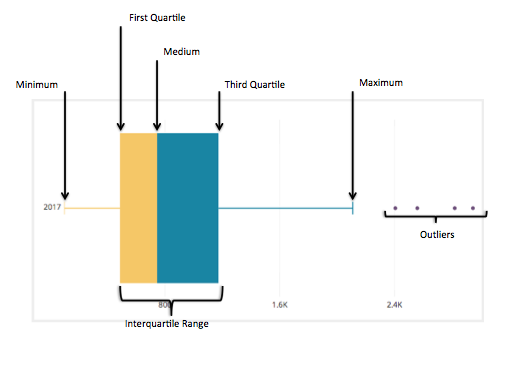
\includegraphics{https://raw.githubusercontent.com/dev7796/data101_tutorial/main/files/img/plots/boxplot1.png}

\begin{itemize}
\tightlist
\item
  A boxplot shows the following things:

  \begin{itemize}
  \tightlist
  \item
    Minimum
  \item
    Maximum
  \item
    Median
  \item
    First quartile
  \item
    Third quartile
  \item
    Outliers
  \end{itemize}
\end{itemize}

eyJsYW5ndWFnZSI6InIiLCJzYW1wbGUiOiIjIG1vb2R5PC1yZWFkLmNzdihcIi4uL2ZpbGVzL2RhdGFzZXQvbW9vZHkyMDIwYi5jc3ZcIikgI3N0YXRpYyBMb2FkXG5tb29keTwtcmVhZC5jc3YoXCJodHRwczovL3Jhdy5naXRodWJ1c2VyY29udGVudC5jb20vZGV2Nzc5Ni9kYXRhMTAxX3R1dG9yaWFsL21haW4vZmlsZXMvZGF0YXNldC9tb29keTIwMjBiLmNzdlwiKSAjd2ViIGxvYWRcbmNvbG9yczwtIGMoJ3JlZCcsJ2JsdWUnLCdjeWFuJywneWVsbG93JywnZ3JlZW4nKSAjIEFzc2lnbmluZyBkaWZmZXJlbnQgY29sb3JzIHRvIGJhcnNcblxuI1N1cHBvc2UgeW91IHdhbnQgdG8gZmluZCB0aGUgZGlzdHJpYnV0aW9uIG9mIHN0dWRlbnRzIHNjb3JlIHBlciBHcmFkZS4gV2UgdXNlIGJveCBwbG90IGZvciBnZXR0aW5nIHRoYXQuIFxuYm94cGxvdChzY29yZX5ncmFkZSxkYXRhPW1vb2R5LHhsYWI9XCJHcmFkZVwiLHlsYWI9XCJTY29yZVwiLCBtYWluPVwiQm94cGxvdCBvZiBncmFkZSB2cyBzY29yZVwiLGNvbD1jb2xvcnMsYm9yZGVyPVwiYmxhY2tcIilcblxuIyB0aGUgY2lyY2xlcyByZXByZXNlbnQgb3V0bGllcnMuIn0=

\begin{center}\rule{0.5\linewidth}{0.5pt}\end{center}

\hypertarget{mosaicplot}{%
\subsection{Mosaic Plot}\label{mosaicplot}}

\begin{itemize}
\tightlist
\item
  Mosaic plot is used to visualize two categorical variables.
\end{itemize}

eyJsYW5ndWFnZSI6InIiLCJzYW1wbGUiOiIjIG1vb2R5PC1yZWFkLmNzdihcIi4uL2ZpbGVzL2RhdGFzZXQvbW9vZHkyMDIwYi5jc3ZcIikgI3N0YXRpYyBMb2FkXG5tb29keTwtcmVhZC5jc3YoXCJodHRwczovL3Jhdy5naXRodWJ1c2VyY29udGVudC5jb20vZGV2Nzc5Ni9kYXRhMTAxX3R1dG9yaWFsL21haW4vZmlsZXMvZGF0YXNldC9tb29keTIwMjBiLmNzdlwiKSAjd2ViIGxvYWRcbmNvbG9yczwtIGMoJ3JlZCcsJ2JsdWUnLCdjeWFuJywneWVsbG93JywnZ3JlZW4nKSAjIEFzc2lnbmluZyBkaWZmZXJlbnQgY29sb3JzIHRvIGJhcnNcblxuI3N1cHBvc2UgeW91IHdhbnQgdG8gZmluZCBudW1iZXJzIG9mIHN0dWRlbnRzIHdpdGggYSBwYXJ0aWN1bGFyIGdyYWRlIGJhc2VkIG9uIHRoZWlyIHRleHRpbmcgaGFiaXRzLiBVc2UgTW9zaWFjLXBsb3QuXG5cbm1vc2FpY3Bsb3QobW9vZHkkZ3JhZGV+bW9vZHkkdGV4dGluZyx4bGFiID0gJ0dyYWRlJyx5bGFiID0gJ1RleHRpbmcgaGFiaXQnLCBtYWluID0gXCJNb3NpYWMgb2YgZ3JhZGUgdnMgdGV4aW5nIGhhYml0IGluIGNsYXNzXCIsY29sPWNvbG9ycyxib3JkZXI9XCJibGFja1wiKSJ9

\hypertarget{additional-references}{%
\subsection{Additional References}\label{additional-references}}

\url{https://www.datamentor.io/r-programming/plot-function/}

\hypertarget{data-transformation}{%
\section{🔖 Data Transformation}\label{data-transformation}}

\begin{itemize}
\tightlist
\item
  \textbf{Lecture slides: } Data Transformation

  \hypertarget{subset12}{}
\end{itemize}

\hypertarget{basic-functions}{%
\subsection{Basic Functions}\label{basic-functions}}

\hypertarget{mean}{%
\subsubsection{mean()}\label{mean}}

\begin{itemize}
\tightlist
\item
  \textbf{mean()} function is used to find the average of values in a numerical vector.
\end{itemize}

eyJsYW5ndWFnZSI6InIiLCJzYW1wbGUiOiJtb29keTwtcmVhZC5jc3YoXCJodHRwczovL3Jhdy5naXRodWJ1c2VyY29udGVudC5jb20vZGV2Nzc5Ni9kYXRhMTAxX3R1dG9yaWFsL21haW4vZmlsZXMvZGF0YXNldC9tb29keTIwMjBiLmNzdlwiKVxuXG4jTGV0cyBsb29rIGF0IHRoZSBtZWFuIG9mIHNjb3JlIGNvbHVtbi5cbm1lYW4obW9vZHkkc2NvcmUpIn0=

\hypertarget{length}{%
\subsubsection{length()}\label{length}}

\begin{itemize}
\tightlist
\item
  \textbf{length()} function is used to get the number of elements in any vector
\end{itemize}

eyJsYW5ndWFnZSI6InIiLCJzYW1wbGUiOiJtb29keTwtcmVhZC5jc3YoXCJodHRwczovL3Jhdy5naXRodWJ1c2VyY29udGVudC5jb20vZGV2Nzc5Ni9kYXRhMTAxX3R1dG9yaWFsL21haW4vZmlsZXMvZGF0YXNldC9tb29keTIwMjBiLmNzdlwiKVxuXG4jTGV0cyBsb29rIGF0IHRoZSBsZW5ndGggb2YgdGhlIGdyYWRlIGNvbHVtbiBcbmxlbmd0aChtb29keSRncmFkZSkifQ==

\hypertarget{max}{%
\subsubsection{max()}\label{max}}

\begin{itemize}
\tightlist
\item
  \textbf{max()} function is used to get the maximum value in a numerical vector.
\end{itemize}

eyJsYW5ndWFnZSI6InIiLCJzYW1wbGUiOiJtb29keTwtcmVhZC5jc3YoXCJodHRwczovL3Jhdy5naXRodWJ1c2VyY29udGVudC5jb20vZGV2Nzc5Ni9kYXRhMTAxX3R1dG9yaWFsL21haW4vZmlsZXMvZGF0YXNldC9tb29keTIwMjBiLmNzdlwiKVxuXG4jbGV0cyBsb29rIGF0IHRoZSBtYXhpbXVtIHZhbHVlIG9mIHRoZSBzY29yZSBpbiB0aGUgc2NvcmUgY29sdW1uXG5tYXgobW9vZHkkc2NvcmUpIn0=

\hypertarget{min}{%
\subsubsection{min()}\label{min}}

\begin{itemize}
\tightlist
\item
  \textbf{min()} function is used to get the minimum value in a numerical vector
\end{itemize}

eyJsYW5ndWFnZSI6InIiLCJzYW1wbGUiOiJtb29keTwtcmVhZC5jc3YoXCJodHRwczovL3Jhdy5naXRodWJ1c2VyY29udGVudC5jb20vZGV2Nzc5Ni9kYXRhMTAxX3R1dG9yaWFsL21haW4vZmlsZXMvZGF0YXNldC9tb29keTIwMjBiLmNzdlwiKVxuXG4jTGV0cyBsb29rIGF0IHRoZSBtaW5pbXVtIHZhbHVlIG9mIHNjb3JlIGluIHRoZSBzY29yZSBjb2x1bW4uXG5taW4obW9vZHkkc2NvcmUpIn0=

\hypertarget{sd}{%
\subsubsection{sd()}\label{sd}}

\begin{itemize}
\tightlist
\item
  \textbf{sd()} function is used to find the standard deviation of numerical vector
\end{itemize}

eyJsYW5ndWFnZSI6InIiLCJzYW1wbGUiOiJtb29keTwtcmVhZC5jc3YoXCJodHRwczovL3Jhdy5naXRodWJ1c2VyY29udGVudC5jb20vZGV2Nzc5Ni9kYXRhMTAxX3R1dG9yaWFsL21haW4vZmlsZXMvZGF0YXNldC9tb29keTIwMjBiLmNzdlwiKVxuXG4jTGV0cyBsb29rIGF0IHRoZSBzdGFuZGFyZCBkZXZpYXRpb24gb2Ygc2NvcmUgY29sdW1uXG5zZChtb29keSRzY29yZSkifQ==

\begin{center}\rule{0.5\linewidth}{0.5pt}\end{center}

\hypertarget{subset}{%
\subsection{Subset}\label{subset}}

\hypertarget{nrow}{%
\subsubsection{Snippet 1- example of subset function}\label{nrow}}

eyJsYW5ndWFnZSI6InIiLCJzYW1wbGUiOiJtb29keTwtcmVhZC5jc3YoXCJodHRwczovL3Jhdy5naXRodWJ1c2VyY29udGVudC5jb20vZGV2Nzc5Ni9kYXRhMTAxX3R1dG9yaWFsL21haW4vZmlsZXMvZGF0YXNldC9NT09EWS0yMDE5LmNzdlwiKVxuI1N1YnNldCBvZiByb3dzXG5tb29keV9uZXZlcl9zbWFydHBob25lPC1zdWJzZXQobW9vZHksT05fU01BUlRQSE9ORT09XCJuZXZlclwiKVxubnJvdyhtb29keSlcbm5yb3cobW9vZHlfbmV2ZXJfc21hcnRwaG9uZSkifQ==

\hypertarget{snippet-2--example-of-subset-function}{%
\subsubsection{Snippet 2- example of subset function}\label{snippet-2--example-of-subset-function}}

eyJsYW5ndWFnZSI6InIiLCJzYW1wbGUiOiJtb29keTwtcmVhZC5jc3YoXCJodHRwczovL3Jhdy5naXRodWJ1c2VyY29udGVudC5jb20vZGV2Nzc5Ni9kYXRhMTAxX3R1dG9yaWFsL21haW4vZmlsZXMvZGF0YXNldC9NT09EWS0yMDE5LmNzdlwiKVxuI1N1YnNldCBvZiByb3dzXG5tb29keTE8LXN1YnNldChtb29keSxPTl9TTUFSVFBIT05FPT1cIm5ldmVyXCIpXG4jIFlvdSBjYW4gc2VlIG9ubHkgc3R1ZGVudCBuZXZlciBvbiBzbWFydHBob25lIGFyZSBpbiB0aGUgc3Vic2V0LlxudGFibGUobW9vZHkxJE9OX1NNQVJUUEhPTkUpICJ9

\hypertarget{snippet-3--subset-as-subframe}{%
\subsubsection{Snippet 3- subset as subframe}\label{snippet-3--subset-as-subframe}}

eyJsYW5ndWFnZSI6InIiLCJzYW1wbGUiOiJtb29keTwtcmVhZC5jc3YoXCJodHRwczovL3Jhdy5naXRodWJ1c2VyY29udGVudC5jb20vZGV2Nzc5Ni9kYXRhMTAxX3R1dG9yaWFsL21haW4vZmlsZXMvZGF0YXNldC9NT09EWS0yMDE5LmNzdlwiKVxuI0FsdGVybmF0ZSB3YXkgdG8gc3Vic2V0LlxubW9vZHkyPC1tb29keVttb29keSRPTl9TTUFSVFBIT05FPT1cIm5ldmVyXCIsIF1cbiMgWW91IGNhbiBzZWUgYSBzaW1pbGFyIHRhYmxlIGFzIGFib3ZlLlxudGFibGUobW9vZHkyJE9OX1NNQVJUUEhPTkUpICJ9

\hypertarget{snippet-4--subsetting-columns}{%
\subsubsection{Snippet 4- subsetting columns}\label{snippet-4--subsetting-columns}}

eyJsYW5ndWFnZSI6InIiLCJzYW1wbGUiOiJtb29keTwtcmVhZC5jc3YoXCJodHRwczovL3Jhdy5naXRodWJ1c2VyY29udGVudC5jb20vZGV2Nzc5Ni9kYXRhMTAxX3R1dG9yaWFsL21haW4vZmlsZXMvZGF0YXNldC9NT09EWS0yMDE5LmNzdlwiKVxuY29sbmFtZXMobW9vZHkpXG4jc3Vic2V0IG9mIGNvbHVtbnNcbm1vb2R5Mzwtc3Vic2V0KG1vb2R5LCBzZWxlY3QgPSAtYygxKSlcbm5jb2wobW9vZHkzKVxuIyBZb3UgY2FuIHNlZSB0aGUgbnVtYmVyIG9mIGNvbHVtbnMgaGFzIGJlZW4gcmVkdWNlZCBieSAxLCBkdWUgdG8gc3ViLXNldHRpbmcgd2l0aG91dCBjb2x1bW4gMVxubmNvbChtb29keTMpIn0=

\hypertarget{snippet-5--sub-setting-rows-and-columns}{%
\subsubsection{Snippet 5- sub-setting rows and columns}\label{snippet-5--sub-setting-rows-and-columns}}

eyJsYW5ndWFnZSI6InIiLCJzYW1wbGUiOiJtb29keTwtcmVhZC5jc3YoXCJodHRwczovL3Jhdy5naXRodWJ1c2VyY29udGVudC5jb20vZGV2Nzc5Ni9kYXRhMTAxX3R1dG9yaWFsL21haW4vZmlsZXMvZGF0YXNldC9NT09EWS0yMDE5LmNzdlwiKVxuI1N1YnNldCBvZiBSb3dzIGFuZCBDb2x1bW5zXG5tb29keTE8LXN1YnNldChtb29keSwgc2VsZWN0ID0gYygyOjQpLCBPTl9TTUFSVFBIT05FID09IFwibmV2ZXJcIilcbmNvbG5hbWVzKG1vb2R5MSlcbiNOb3RpY2UgdGhhdCBvbmx5IDMgY29sdW1ucyBhcmUgcmVtYWluaW5nXG5kaW0obW9vZHkxKSJ9

\hypertarget{code-review-1}{%
\subsubsection{Code Review}\label{code-review-1}}

\hypertarget{what-would-r-say-2}{%
\paragraph{What would R say?}\label{what-would-r-say-2}}

eyJsYW5ndWFnZSI6InIiLCJzYW1wbGUiOiJtb29keTwtcmVhZC5jc3YoXCJodHRwczovL3Jhdy5naXRodWJ1c2VyY29udGVudC5jb20vZGV2Nzc5Ni9kYXRhMTAxX3R1dG9yaWFsL21haW4vZmlsZXMvZGF0YXNldC9NT09EWS0yMDE5LmNzdlwiKVxubW9vZHlbbW9vZHkkU0NPUkU+PTkwLDNdXG4jIFdoYXQgd2lsbCBSIHNheT9cblxuXG4jIEEuIEdldCBzdWJzZXQgb2YgYWxsIGNvbHVtbnMgd2hpY2ggY29udGFpbnMgc3R1ZGVudHMgd2hvIHNjb3JlZCBtb3JlIHRoYW4gZXF1YWwgdG8gOTBcbiMgQi4gZXJyb3JcbiMgQy4gZ2V0IGFsbCBzY29yZSB2YWx1ZXMgd2hpY2ggYXJlIG1vcmUgdGhhbiBlcXVhbCB0byA5MFxuIyBELiBnZXQgc3Vic2V0IG9mIG9ubHkgdGhlIGdyYWRlcyBvZiBzdHVkZW50cyB3aXRoIHNjb3JlIGdyZWF0ZXIgdGhhbiBlcXVhbCB0byA5MCJ9

\hypertarget{what-would-r-say-3}{%
\paragraph{What would R say?}\label{what-would-r-say-3}}

eyJsYW5ndWFnZSI6InIiLCJzYW1wbGUiOiJtb29keTwtcmVhZC5jc3YoXCJodHRwczovL3Jhdy5naXRodWJ1c2VyY29udGVudC5jb20vZGV2Nzc5Ni9kYXRhMTAxX3R1dG9yaWFsL21haW4vZmlsZXMvZGF0YXNldC9NT09EWS0yMDE5LmNzdlwiKVxuXG5tb29keVttb29keSRTQ09SRT49ODAuMCAmIG1vb2R5JEdSQURFID09J0InLF0gXG4jIFdoYXQgd2lsbCBSIHNheT9cblxuIyBBLiBzdWJzZXQgb2YgbW9vZHkgZGF0YSBmcmFtZSB3aG8gZ290IEIgZ3JhZGUuXG4jIEIuIGVycm9yLlxuIyBDLiBzdWJzZXQgb2YgbW9vZHkgZGF0YSBmcmFtZSB3aXRoIHNjb3JlIGdyZWF0ZXIgdGhhbiA4MC5cbiMgRC4gc3Vic2V0IG9mIG1vb2R5IGRhdGEgZnJhbWUgd2l0aCBzY29yZSBtb3JlIHRoYW4gODAgYW5kIGdvdCBCIGdyYWRlLiJ9

\begin{center}\rule{0.5\linewidth}{0.5pt}\end{center}

\hypertarget{tapply}{%
\subsection{tapply}\label{tapply}}

\begin{itemize}
\tightlist
\item
  \textbf{tapply()} computes a measure (mean, median, min, max, etc..) or a function for each factor variable in a vector. It is a very useful function that lets you create a subset of a vector and then apply some functions to each of the subset.
\item
  tapply(numerical, categorical, aggregagte function)
\end{itemize}

\hypertarget{snippet-1--example-of-tapply-followed-by-barplot}{%
\subsubsection{Snippet 1- Example of tapply followed by barplot}\label{snippet-1--example-of-tapply-followed-by-barplot}}

eyJsYW5ndWFnZSI6InIiLCJzYW1wbGUiOiJtb29keTwtcmVhZC5jc3YoXCJodHRwczovL3Jhdy5naXRodWJ1c2VyY29udGVudC5jb20vZGV2Nzc5Ni9kYXRhMTAxX3R1dG9yaWFsL21haW4vZmlsZXMvZGF0YXNldC9NT09EWS0yMDE5LmNzdlwiKVxuXG5cbiMgVG8gYXBwbHkgdGFwcGx5KCkgb24gU0NPUkUgZmFjdG9yZWQgb24gT05fU01BUlRQSE9ORVxuXG5tb29keTE8LXRhcHBseShtb29keSRTQ09SRSxtb29keSRPTl9TTUFSVFBIT05FLG1lYW4pXG5tb29keTEgIyBXZSBjYW4gc2VlIGl0IGNhbGN1bGF0ZWQgbWVhbiB2YWx1ZSBvZiB0aGUgc2NvcmUgYnkgc3R1ZGVudHMgd2l0aCByZXNwZWN0IHRvIHRoZWlyIHVzZSBvZiBwaG9uZSBpbiBjbGFzcy5cblxuYmFycGxvdChtb29keTEsY29sID0gXCJjeWFuXCIseGxhYiA9IFwiTGFiZWxzXCIsIHlsYWIgPSBcIm1lYW5fdmFsXCIsbWFpbiA9IFwidGFwcGx5KCkgZXhhbXBsZSAxXCIsbGFzID0gMiwgY2V4Lm5hbWVzID0gMC43NSkjcGxvdCJ9

\hypertarget{code-review-2}{%
\subsubsection{Code Review}\label{code-review-2}}

\hypertarget{what-would-r-say-4}{%
\paragraph{What would R say?}\label{what-would-r-say-4}}

eyJsYW5ndWFnZSI6InIiLCJzYW1wbGUiOiJtb29keTwtcmVhZC5jc3YoXCJodHRwczovL3Jhdy5naXRodWJ1c2VyY29udGVudC5jb20vZGV2Nzc5Ni9kYXRhMTAxX3R1dG9yaWFsL21haW4vZmlsZXMvZGF0YXNldC9NT09EWS0yMDE5LmNzdlwiKVxuXG50YXBwbHkobW9vZHksIEdSQURFLCBTQ09SRSwgbWluKVxuIyBXaGF0IHdpbGwgUiBzYXk/XG5cbiMgQS4gbWluaW11bSBzY29yZSBmb3IgZWFjaCBncmFkZVxuIyBCLiBtaW5pbXVtIGdyYWRlIGZvciBlYWNoIHNjb3JlXG4jIEMuIG1pbmltdW0gZ3JhZGUgb25seSBcbiMgRC4gRXJyb3IuIn0=

\begin{center}\rule{0.5\linewidth}{0.5pt}\end{center}

\hypertarget{derived-attribute}{%
\subsection{Derived Attribute}\label{derived-attribute}}

R allows creating new data frame attributes (columns) ``on the fly''. These are new vectors, which are often defined as functions of existing attributes. Hence, the name - derived attributes.

Derived attributes will play an important role in data exploration as well as in building prediction models. Very often, derived attributes allow discovery of important patterns in data. Similarly, derived attributes may be more predictive than original attributes in the imported data sets.

The term feature engineering is often used in machine learning to describe creation of derived attributes.

\hypertarget{snippet-1---making-new-categorical-attribute.}{%
\subsubsection{Snippet 1 - Making new categorical attribute.}\label{snippet-1---making-new-categorical-attribute.}}

The line 4 initializes the new attribute PF (Pass/Fail) to ``Pass''. The line 5 replaces ``Pass'' by ``Fail'' for students who received F. This new attribute, PF, will allow exploratory analysis to find ``How to pass Professor Moody's class''. The answer to this question may be different than then answer to ``How to get a good grade in Professor Moody's class''.

eyJsYW5ndWFnZSI6InIiLCJzYW1wbGUiOiJtb29keTwtcmVhZC5jc3YoXCJodHRwczovL3Jhdy5naXRodWJ1c2VyY29udGVudC5jb20vZGV2Nzc5Ni9kYXRhMTAxX3R1dG9yaWFsL21haW4vZmlsZXMvZGF0YXNldC9NT09EWS0yMDE5LmNzdlwiKVxuXG4jIEN1dCBFeGFtcGxlIHVzaW5nIGJyZWFrcyAtIEN1dHRpbmcgZGF0YSB1c2luZyBkZWZpbmVkIHZlY3Rvci4gXG5tb29keSRQRjwtJ1Bhc3MnXG5tb29keVttb29keSRHUkFERT09J0YnLF0kUEY8LSdGYWlsJ1xuXG4jIGxldHMgc2VlIG91ciBhZGRlZCBjb2x1bW4gUEZcbm1vb2R5In0=

\hypertarget{cut}{%
\subsubsection{Cut}\label{cut}}

\begin{itemize}
\tightlist
\item
  \textbf{cut()} function divides the range of x into intervals. Provides ability to label intervals as well. It plays important role in defining derived attributes from attributes which are numerical.
\end{itemize}

eyJsYW5ndWFnZSI6InIiLCJzYW1wbGUiOiJtb29keTwtcmVhZC5jc3YoXCJodHRwczovL3Jhdy5naXRodWJ1c2VyY29udGVudC5jb20vZGV2Nzc5Ni9kYXRhMTAxX3R1dG9yaWFsL21haW4vZmlsZXMvZGF0YXNldC9NT09EWS0yMDE5LmNzdlwiKVxuXG4jIEN1dCBFeGFtcGxlIHVzaW5nIGJyZWFrcyAtIEN1dHRpbmcgZGF0YSB1c2luZyBkZWZpbmVkIHZlY3Rvci4gXG5zY29yZTEgPC0gY3V0KG1vb2R5JFNDT1JFLGJyZWFrcz1jKDAsNTAsMTAwKSxsYWJlbHM9YyhcIkZcIixcIlBcIikpXG50YWJsZShzY29yZTEpIn0=

\hypertarget{code-review-3}{%
\subsubsection{Code Review}\label{code-review-3}}

\hypertarget{what-would-r-say-5}{%
\paragraph{What would R say?}\label{what-would-r-say-5}}

eyJsYW5ndWFnZSI6InIiLCJzYW1wbGUiOiJtb29keTwtcmVhZC5jc3YoXCJodHRwczovL3Jhdy5naXRodWJ1c2VyY29udGVudC5jb20vZGV2Nzc5Ni9kYXRhMTAxX3R1dG9yaWFsL21haW4vZmlsZXMvZGF0YXNldC9NT09EWS0yMDE5LmNzdlwiKVxuXG5jdXQobW9vZHkkU0NPUkUsIGJyZWFrcz1jKDAsMjUsNzAsMTAwKSxsYWJlbHM9YyhcImxvd1wiLCBcIm1lZGl1bVwiLCBcImhpZ2hcIikpXG4jV2hhdCB3b3VsZCBSIHNheT9cblxuIyBBLiA1IGludGVydmFscyBvZiBhdHRyaWJ1dGUgc2NvcmVcbiMgQi4gMyBpbnRlcnZhbHMgKDAsMjUpICgyNSw3MCkgKDc1LDEwMClcbiMgQy4gMyBjYXRlZ29yaWNhbCB2YWx1ZXMgXCJsb3dcIiwgXCJtZWRpdW1cIiBhbmQgXCJoaWdoXCIgZm9yIGRpZmZlcmVudCBzY29yZSBpbnRlcnZhbHNcbiMgRC4gMyBzZXBhcmF0ZSBkYXRhc2V0cyB3aXRoIHNpbWlsYXIgc2NvcmUgdmFsdWVzIn0=

\hypertarget{what-would-r-say-6}{%
\paragraph{What would R say?}\label{what-would-r-say-6}}

eyJsYW5ndWFnZSI6InIiLCJzYW1wbGUiOiJtb29keTwtcmVhZC5jc3YoXCJodHRwczovL3Jhdy5naXRodWJ1c2VyY29udGVudC5jb20vZGV2Nzc5Ni9kYXRhMTAxX3R1dG9yaWFsL21haW4vZmlsZXMvZGF0YXNldC9NT09EWS0yMDE5LmNzdlwiKVxuXG5vdXRwdXQ8LWN1dChtb29keSRTQ09SRSwgNSlcbnN1bW1hcnkob3V0cHV0KVxuI1doYXQgd291bGQgUiBzYXk/XG5cbiMgQS4gNSBpbnRlcnZhbHMgb2YgYXR0cmlidXRlIHNjb3JlIG9mIHVuZXF1YWwgY291bnQgb2YgZWxlbWVudHNcbiMgQi4gNSBpbnRlcnZhbHMgb2YgYXR0cmlidXRlIHNjb3JlIG9mIGVxdWFsIGNvdW50IG9mIGVsZW1lbnRzXG4jIEMuIDUgY2F0ZWdvcmljYWwgdmFsdWVzIGZvciBkaWZmZXJlbnQgc2NvcmUgaW50ZXJ2YWxzXG4jIEQuIDUgc2VwYXJhdGUgZGF0YXNldCB3aXRoIHNpbWlsYXIgc2NvcmUgdmFsdWVzIn0=

\hypertarget{what-would-r-say-7}{%
\paragraph{What would R say?}\label{what-would-r-say-7}}

eyJsYW5ndWFnZSI6InIiLCJzYW1wbGUiOiJtb29keTwtcmVhZC5jc3YoXCJodHRwczovL3Jhdy5naXRodWJ1c2VyY29udGVudC5jb20vZGV2Nzc5Ni9kYXRhMTAxX3R1dG9yaWFsL21haW4vZmlsZXMvZGF0YXNldC9NT09EWS0yMDE5LmNzdlwiKVxuXG5vdXRwdXQ8LWN1dChtb29keSRBU0tTX1FVRVNUSU9OUywgMilcbnN1bW1hcnkob3V0cHV0KVxuI1doYXQgd291bGQgUiBzYXk/XG5cbiMgQS4gMiBpbnRlcnZhbHMgb2YgYXR0cmlidXRlIGFza19xdWVzdGlvbnMgb2YgdW5lcXVhbCBjb3VudCBvZiBlbGVtZW50cyBpbiBlYWNoIGludGVydmFsXG4jIEIuIDIgaW50ZXJ2YWxzIG9mIGF0dHJpYnV0ZSBhc2tfcXVlc3Rpb25zIG9mIGVxdWFsIGNvdW50IG9mIGVsZW1lbnRzIGluIGVhY2ggaW50ZXJ2YWxcbiMgQy4gMiBjYXRlZ29yaWNhbCB2YWx1ZXMgZm9yIGRpZmZlcmVudCBhc2tfcXVlc3Rpb25zIGludGVydmFsc1xuIyBELiBFcnJvci4ifQ==

\hypertarget{more-complex-example-of-defining-derived-attributes}{%
\paragraph{More complex example of defining derived attributes}\label{more-complex-example-of-defining-derived-attributes}}

The next snippet illustrates defining a new numerical attribute, \$adjustedScore of a student in the Moody data frame.

Score is adjusted by the value of participation attribute in the following way:

\begin{itemize}
\item
  If participation is larger than 0.5 - a bonus proportional to participation * 10 is added to the score.
\item
  If participation is smaller than 0.5, a penalty of 1-participation) * 10 is subtracted from the score.
\end{itemize}

In this way, for someone with very small participation, the 10 point penalty will be imposed (10 points subtracted from the score). Conversely, someone with perfect participation (1.0) will receive a 10 point bonus.

\hypertarget{snippet-1-3}{%
\subparagraph{Snippet 1}\label{snippet-1-3}}

eyJsYW5ndWFnZSI6InIiLCJzYW1wbGUiOiJtb29keTwtcmVhZC5jc3YoXCJodHRwczovL3Jhdy5naXRodWJ1c2VyY29udGVudC5jb20vZGV2Nzc5Ni9kYXRhMTAxX3R1dG9yaWFsL21haW4vZmlsZXMvZGF0YXNldC9tb29keTIwMjBiLmNzdlwiKVxuXG5cbm1vb2R5JGNvbmRpdGlvbmFsIDwtMFxubW9vZHlbbW9vZHkkcGFydGljaXBhdGlvbjwwLjUwLCBdJGNvbmRpdGlvbmFsIDwtIG1vb2R5W21vb2R5JHBhcnRpY2lwYXRpb248MC41MCwgXSRzY29yZSAtMTAqKDEtbW9vZHlbbW9vZHkkcGFydGljaXBhdGlvbjwwLjUwLCBdJHBhcnRpY2lwYXRpb24pXG5tb29keVttb29keSRwYXJ0aWNpcGF0aW9uPj0wLjUwLCBdJGNvbmRpdGlvbmFsIDwtIG1vb2R5W21vb2R5JHBhcnRpY2lwYXRpb24+PTAuNTAsIF0kc2NvcmUgKzEwKm1vb2R5W21vb2R5JHBhcnRpY2lwYXRpb24+PTAuNTAsIF0kcGFydGljaXBhdGlvblxuXG4jIHByaW50IHRoZSBjb2x1bW4gbmFtZXNcbmNvbG5hbWVzKG1vb2R5KVxuXG4jIGxldHMgbG9vayBhdCB0aGUgY29uZGl0aW9uYWwgYXR0cmlidXRlIFxuaGVhZChtb29keSlcblxuI3N1YnNldCB0aGUgbW9vZHkgZGF0YXNldCByb3dzID0gMSB0byAxMCBhbmQgY29scyA9IDEsNVxubW9vZHlbMToxMCwgYygxLDUpXVxuXG4jc3Vic2V0IHRoZSBtb29keSBkYXRhc2V0IHJvd3MgPSAxIHRvIDEwIGFuZCBjb2xzID0gMSw1LDZcbm1vb2R5WzE6MTAsIGMoMSw1LDYpXVxuXG4jIHByaW50IHN1bW1hcnkgb2YgaW5pZGl2aWR1YWwgY29sdW1uc1xuc3VtbWFyeShtb29keSRzY29yZSlcbnN1bW1hcnkobW9vZHkkY29uZGl0aW9uYWwpXG5cbiMgUGxvdHRpbmcgdGhlIGNvbmRpdGlvbmFsIGF0dHJpYnV0ZSB1c2luZyBib3hwbG90XG5ib3hwbG90KG1vb2R5JGNvbmRpdGlvbmFsLGNvbCA9IGMoXCJyZWRcIiksbWFpbj1cIkNvbXBsZXggRXhhbXBsZVwiKVxuXG4jIFBsb3R0aW5nIHRoZSBzY29yZSBhdHRyaWJ1dGUgdXNpbmcgYm94cGxvdFxuYm94cGxvdChtb29keSRzY29yZSxjb2wgPSBjKFwiYmx1ZVwiKSxtYWluPVwiQ29tcGxleCBFeGFtcGxlXCIpIn0=

\hypertarget{ztest}{%
\section{🔖 Hypothesis Testing: z-test}\label{ztest}}

\begin{itemize}
\tightlist
\item
  \textbf{Lecture slides: } Hypothesis Testing Central Limit Theorem

  \hypertarget{HPT12}{}

  \hypertarget{CLT12}{}
\end{itemize}

\begin{itemize}
\tightlist
\item
  \textbf{Great Resource: } Khan Academy
\end{itemize}

\hypertarget{introduction}{%
\subsection{Introduction}\label{introduction}}

The following synthetic data describes daily traffic on weekday and weekend days in Lincoln and Holland tunnels. The data frame has three attributes: TUNNEL, DAY and VOLUME\_PER\_MINUTE. Below we show a small sample of the TRAFFIC data frame

\begin{table}

\caption{\label{tab:unnamed-chunk-83}Snippet of Traffic Dataset}
\centering
\begin{tabular}[t]{lllr}
\toprule
  & TUNNEL & DAY & VOLUME\_PER\_MINUTE\\
\midrule
408 & Holland & weekday & 70.5\\
1995 & Lincoln & weekday & 69.0\\
2095 & Lincoln & weekday & 77.0\\
828 & Holland & weekday & 70.5\\
2353 & Lincoln & weekday & 74.0\\
\addlinespace
1529 & Lincoln & weekday & 73.0\\
392 & Holland & weekday & 46.5\\
1915 & Lincoln & weekday & 66.0\\
2562 & Lincoln & weekend & 80.0\\
740 & Holland & weekday & 95.5\\
\bottomrule
\end{tabular}
\end{table}

The following snippet \textbf{6.2} shows the code for hypothesis test of difference of means.

Is the mean traffic (VOLUME\_PER\_MINUTE) in the Holland tunnel bigger than mean traffic (VOLUME\_PER\_MINUTE) in the Lincoln?

\hypertarget{pnorm}{%
\subsection{Snippet 1: Shows the code for z-test to test the following hypotheses}\label{pnorm}}

\textbf{Null Hypothesis} - Traffic in Holland tunnel is the same as traffic in Lincoln tunnel.

\textbf{Alternative Hypothesis} - Traffic in the Holland Tunnel is larger than traffic in the Lincoln tunnel.

In the snippet \textbf{6.2} we end up calculating the p-value which leads to rejection of Null hypothesis (good news for data scientist, bad for the sceptic). Indeed, p-value is less than the significance level of 5\%.
This means, that under null hypothesis it is extremely unlikely (less than 5\% chance) to see the result which is at least as big as the observed difference of means.

eyJsYW5ndWFnZSI6InIiLCJzYW1wbGUiOiJUUkFGRklDPC1yZWFkLmNzdignaHR0cHM6Ly9yYXcuZ2l0aHVidXNlcmNvbnRlbnQuY29tL2Rldjc3OTYvZGF0YTEwMV90dXRvcmlhbC9tYWluL2ZpbGVzL2RhdGFzZXQvVHJhZmZpYzIwMjIuY3N2JylcblxuI2RhdGEgY2xlYW4gYW5kIHN1YnNldCwgZWl0aGVyXG5saW5jb2xuLmRhdGEgPC0gc3Vic2V0KFRSQUZGSUMsIFRSQUZGSUMkVFVOTkVMID09IFwiTGluY29sblwiKVxuaG9sbGFuZC5kYXRhIDwtIHN1YnNldChUUkFGRklDLCBUUkFGRklDJFRVTk5FTCA9PSBcIkhvbGxhbmRcIilcblxuI3RyYWZmaWMgYXQgbGluY29sblxubGluY29sbi50cmFmZmljIDwtIGxpbmNvbG4uZGF0YSRWT0xVTUVfUEVSX01JTlVURVxuXG4jdHJhZmZpYyBhdCBob2xsYW5kXG5ob2xsYW5kLnRyYWZmaWMgPC0gaG9sbGFuZC5kYXRhJFZPTFVNRV9QRVJfTUlOVVRFXG5cbiMgc3RhbmRhcmQgZGV2aWF0aW9uIG9mIHR3byBzYW1wbGVzLlxuc2QubGluY29sbiA8LSBzZChsaW5jb2xuLnRyYWZmaWMpXG5zZC5ob2xsYW5kIDwtIHNkKGhvbGxhbmQudHJhZmZpYylcbnNkLmxpbmNvbG5cbnNkLmhvbGxhbmRcblxuI2xlbmd0aCBvZiBsaW5jb2xuIGFuZCBob2xsYW5kXG5sZW5fbGluY29sbiA8LSBsZW5ndGgobGluY29sbi50cmFmZmljKVxubGVuX2hvbGxhbmQgPC0gbGVuZ3RoKGhvbGxhbmQudHJhZmZpYylcbmxlbl9saW5jb2xuXG5sZW5faG9sbGFuZFxuXG4jc3RhbmRhcmQgZGV2aWF0aW9uIG9mIGRpZmZlcmVuY2UgdHJhZmZpY1xuc2QubGluLmhvbCA8LSBzcXJ0KHNkLmxpbmNvbG5eMi9sZW5fbGluY29sbiArIHNkLmhvbGxhbmReMi9sZW5faG9sbGFuZClcbnNkLmxpbi5ob2xcblxuI21lYW5zIG9mIHR3byBzYW1wbGVzXG5tZWFuLmxpbmNvbG4gPC0gbWVhbihsaW5jb2xuLnRyYWZmaWMpXG5tZWFuLmhvbGxhbmQgPC0gbWVhbihob2xsYW5kLnRyYWZmaWMpXG5tZWFuLmxpbmNvbG5cbm1lYW4uaG9sbGFuZFxuXG4jeiBzY29yZVxuemV0YSA8LSAobWVhbi5saW5jb2xuIC0gbWVhbi5ob2xsYW5kKS9zZC5saW4uaG9sXG56ZXRhXG5cbiNwbG90IHJlZCBsaW5lXG5wbG90KHg9c2VxKGZyb20gPSAtNSwgdG89IDUsIGJ5PTAuMSkseT1kbm9ybShzZXEoZnJvbSA9IC01LCB0bz0gNSwgIGJ5PTAuMSksbWVhbj0wKSx0eXBlPSdsJyx4bGFiID0gJ21lYW4gZGlmZmVyZW5jZScsICB5bGFiPSdwb3NzaWJpbGl0eScpXG5hYmxpbmUodj16ZXRhLCBjb2w9J3JlZCcpXG5cbiNnZXQgcFxucCA9IDEtcG5vcm0oemV0YSlcbnAifQ==

\hypertarget{snippet-2-make-your-own-data-and-see-how-p-value-changes}{%
\subsection{Snippet 2: Make your own data and see how p-value changes}\label{snippet-2-make-your-own-data-and-see-how-p-value-changes}}

How p-value is affected by difference of means and standard deviations.

We will build two distributions ourselves - varying the means and standard deviations. We will use \textbf{rnorm()} to generate normal distributions with given means and standard deviations. Then we will use a permutation test (can be a z-test as well) to test the difference of means for these two synthetic distributions. See for yourself the impact means and standard deviations have on p-values. You can do it by changing values of mean and standard deviation in the \textbf{rnorm()} function.

Clearly the further apart the mean values are - the lower the p-value. But how do standard deviations affect the p-value? See for yourself.

Build the data frame with two attributes: Cat and Val, using \textbf{rnorm()} function

eyJsYW5ndWFnZSI6InIiLCJzYW1wbGUiOiJWYWwxPC1ybm9ybSgxMCxtZWFuPTI1LCBzZD0xMClcblZhbDI8LXJub3JtKDEwLG1lYW49MzUsIHNkPTEwKVxuQ2F0MTwtcmVwKFwiR3JvdXBBXCIsMTApICBcbkNhdDI8LXJlcChcIkdyb3VwQlwiLDEwKSAgXG5DYXQ8LWMoQ2F0MSxDYXQyKSBcblZhbDwtYyhWYWwxLFZhbDIpXG5cbmQ8LWRhdGEuZnJhbWUoQ2F0LFZhbClcbk9ic2VydmVkX0RpZmZlcmVuY2U8LW1lYW4oZFtkJENhdD09J0dyb3VwQicsMl0pLW1lYW4oZFtkJENhdD09J0dyb3VwQScsMl0pXG5PYnNlcnZlZF9EaWZmZXJlbmNlXG5cbmRBPC1kW2QkQ2F0PT0nR3JvdXBBJyxdXG5kQVxuZEI8LWRbZCRDYXQ9PSdHcm91cEInLF1cbmRCXG5cbm1lYW5BPC1tZWFuKGRBJFZhbClcbm1lYW5CPC1tZWFuKGRCJFZhbClcblxuc2RBPC1zZChkQSRWYWwpXG5zZEI8LXNkKGRCJFZhbClcblxubGVuQTwtbnJvdyhkQSlcbmxlbkFcbmxlbkI8LW5yb3coZEIpXG5sZW5CXG5cbnNkLkEuQiA8LSBzcXJ0KHNkQV4yL2xlbkEgK3NkQl4yL2xlbkIpXG5zZC5BLkJcblxuemV0YSA8LSAobWVhbkIgLSBtZWFuQSkvc2QuQS5CXG56ZXRhXG5wPC0xLXBub3JtKHpldGEpXG5wIn0=

\hypertarget{additional-references-1}{%
\subsection{Additional References}\label{additional-references-1}}

\url{https://www.statisticshowto.com/probability-and-statistics/statistics-definitions/p-value/}
\url{http://www.z-table.com/}
\url{https://www.statisticshowto.com/probability-and-statistics/z-score/}
\url{https://sixsigmastudyguide.com/z-scores-z-table-z-transformations/}

\hypertarget{ptest}{%
\section{🔖 Hypothesis Testing: Permutation Test}\label{ptest}}

\begin{itemize}
\tightlist
\item
  \textbf{Lecture slides: } Permutation Test

  \hypertarget{PT12}{}
\end{itemize}

\hypertarget{snippet-1-4}{%
\subsection{Snippet 1}\label{snippet-1-4}}

\textbf{Exercise} - How p-value is affected by difference of means and standard deviations

We will build our two distributions ourseleves - varying the means and standard deviations. We will use \textbf{rnorm()} to generate normal distributions with given means and standard deviations. Then we will use permutation test (can be z-test as well) to test difference of means for these two synthetic distributions. See for yourself the impact means and standard deviations have on p-values.

Build the data frame with two attributes: \textbf{Cat} and \textbf{Val}, using \textbf{rnorm()} function

eyJsYW5ndWFnZSI6InIiLCJzYW1wbGUiOiJWYWwxPC1ybm9ybSgxMCxtZWFuPTI1LCBzZD0xMClcblZhbDI8LXJub3JtKDEwLG1lYW49MzAsIHNkPTEwKVxuIFxuQ2F0MTwtcmVwKFwiR3JvdXBBXCIsMTApICAjIGZvciBleGFtcGxlIEdyb3VwQSBjYW4gYmUgSG9sbGFuZCBUdW5uZWxcbkNhdDI8LXJlcChcIkdyb3VwQlwiLDEwKSAgIyBmb3IgZXhhbXBsZSBHcm91cCBCIHdpbGwgYmUgTGluY29sbiBUdW5uZWxcblxuQ2F0MVxuQ2F0MlxuXG4jVGhlIHJlcCBjb21tYW5kIHdpbGwgcmVwZWF0LCB0aGUgdmFyaWFibGVzIHdpbGwgYmUgb2YgdHlwZSBjaGFyYWN0ZXIgYW5kIHdpbGwgY29udGFpbiAxMCB2YWx1ZXMgZWFjaC5cblxuQ2F0PC1jKENhdDEsQ2F0MikgIyBBIHZhcmlhYmxlIHdpdGggZmlyc3QgMTAgdmFsdWVzIEdyb3VwQSBhbmQgbmV4dCAxMCB2YWx1ZXMgR3JvdXBCXG5DYXRcblxuVmFsPC1jKFZhbDEsVmFsMilcblZhbFxuXG5kPC1kYXRhLmZyYW1lKENhdCxWYWwpXG5kXG5cbk9ic2VydmVkX0RpZmZlcmVuY2U8LW1lYW4oZFtkJENhdD09J0dyb3VwQicsMl0pLW1lYW4oZFtkJENhdD09J0dyb3VwQScsMl0pXG5PYnNlcnZlZF9EaWZmZXJlbmNlXG5cbiNUaGlzIHdpbGwgY2FsY3VsYXRlIHRoZSBtZWFuIG9mIHRoZSBzZWNvbmQgY29sdW1uIChoYXZpbmcgMTAgcmFuZG9tIHZhbHVlcyBmb3IgZWFjaCBncm91cCksIGFuZCB0aGUgbWVhbiBvZiBncm91cEIgdmFsdWVzIGlzIHN1YnRyYWN0ZWQgZnJvbSB0aGUgbWVhbiBvZiBncm91cEEgdmFsdWVzLCB3aGljaCB3aWxsIGdpdmUgeW91IHRoZSB2YWx1ZSBvZiB0aGUgZGlmZmVyZW5jZSBvZiB0aGUgbWVhbi5cbiBcbiAjVHJ5IGNoYW5naW5nIG1lYW4gYW5kIHNkIHZhbHVlcy4gV2hlbiB5b3UgcnVuIHRoaXMgeW91IHdpbGwgc2VlIHRoYXQgdGhlIGRpZmZlcmVuY2UgaXMgc29tZXRpbWVzIG5lZ2F0aXZlICNvciBzb21ldGltZXMgcG9zaXRpdmUuIn0=

\hypertarget{snippet-2-2}{%
\subsection{Snippet 2}\label{snippet-2-2}}

Do this in your R studio, since we cannot install our package in data camp service we are using to run the code snippets

eyJsYW5ndWFnZSI6InIiLCJwcmVfZXhlcmNpc2VfY29kZSI6InRyYWZmaWM8LXJlYWQuY3N2KCdodHRwczovL3Jhdy5naXRodWJ1c2VyY29udGVudC5jb20va3VuYWwwODk1L1JEYXRhc2V0cy9tYXN0ZXIvVFJBRkZJQy5jc3YnKVxuUGVybXV0YXRpb24gPC0gZnVuY3Rpb24oZGYxLGMxLGMyLG4sdzEsdzIpe1xuICBkZiA8LSBhcy5kYXRhLmZyYW1lKGRmMSlcbiAgRF9udWxsPC1jKClcbiAgVjE8LWRmWyxjMV1cbiAgVjI8LWRmWyxjMl1cbiAgc3ViLnZhbHVlMSA8LSBkZltkZlssIGMxXSA9PSB3MSwgYzJdXG4gIHN1Yi52YWx1ZTIgPC0gZGZbZGZbLCBjMV0gPT0gdzIsIGMyXVxuICBEIDwtICBhYnMobWVhbihzdWIudmFsdWUyLCBuYS5ybT1UUlVFKSAtIG1lYW4oc3ViLnZhbHVlMSwgbmEucm09VFJVRSkpXG4gIG09bGVuZ3RoKFYxKVxuICBsPWxlbmd0aChWMVtWMT09dzJdKVxuICBmb3IoamogaW4gMTpuKXtcbiAgICBudWxsIDwtIHJlcCh3MSxsZW5ndGgoVjEpKVxuICAgIG51bGxbc2FtcGxlKG0sbCldIDwtIHcyXG4gICAgbmYgPC0gZGF0YS5mcmFtZShLZXk9bnVsbCwgVmFsdWU9VjIpXG4gICAgbmFtZXMobmYpIDwtIGMoXCJLZXlcIixcIlZhbHVlXCIpXG4gICAgdzFfbnVsbCA8LSBuZltuZiRLZXkgPT0gdzEsMl1cbiAgICB3Ml9udWxsIDwtIG5mW25mJEtleSA9PSB3MiwyXVxuICAgIERfbnVsbCA8LSBjKERfbnVsbCxtZWFuKHcyX251bGwsIG5hLnJtPVRSVUUpIC0gbWVhbih3MV9udWxsLCBuYS5ybT1UUlVFKSlcbiAgfVxuICBteWhpc3Q8LWhpc3QoRF9udWxsLCBwcm9iPVRSVUUpXG4gIG11bHRpcGxpZXIgPC0gbXloaXN0JGNvdW50cyAvIG15aGlzdCRkZW5zaXR5XG4gIG15ZGVuc2l0eSA8LSBkZW5zaXR5KERfbnVsbCwgYWRqdXN0PTIpXG4gIG15ZGVuc2l0eSR5IDwtIG15ZGVuc2l0eSR5ICogbXVsdGlwbGllclsxXVxuICBwbG90KG15aGlzdClcbiAgbGluZXMobXlkZW5zaXR5LCBjb2w9J2JsdWUnKVxuICBhYmxpbmUodj1ELCBjb2w9J3JlZCcpXG4gIE08LW1lYW4oRF9udWxsPkQpXG4gIHJldHVybihNKVxufSIsInNhbXBsZSI6IiNpbnN0YWxsLnBhY2thZ2VzKFwiZGV2dG9vbHNcIilcbiNkZXZ0b29sczo6aW5zdGFsbF9naXRodWIoXCJkZXZhbnNoYWdyL1Blcm11dGF0aW9uVGVzdFNlY29uZFwiKVxuXG4jUGVybXV0YXRpb25UZXN0U2Vjb25kOjpQZXJtdXRhdGlvbihkLCBcIkNhdFwiLCBcIlZhbFwiLDEwMDAwLCBcIkdyb3VwQVwiLCBcIkdyb3VwQlwiKVxuUGVybXV0YXRpb24odHJhZmZpYywgXCJUVU5ORUxcIiwgXCJWT0xVTUVfUEVSX01JTlVURVwiLDEwMDAsXCJIb2xsYW5kXCIsIFwiTGluY29sblwiKVxuIFxuICNUaGUgUGVybXV0YXRpb24gZnVuY3Rpb24gcmV0dXJucyB0aGUgYWJzb2x1dGUgdmFsdWUgb2YgdGhlIGRpZmZlcmVuY2UuIFNvIHRoZSByZWQgbGluZSBpcyB0aGUgYWJzb2x1dGUgdmFsdWUgb2YgdGhlIG9ic2VydmVkIGRpZmZlcmVuY2UuIFlvdSB3aWxsIHNlZSBhIGhpc3RvZ3JhbSBoYXZpbmcgYSBub3JtYWwgZGlzdHJpYnV0aW9uIHdpdGggYSByZWQgc2hvd2luZyB0aGUgb2JzZXJ2ZWQgZGlmZmVyZW5jZS4ifQ==

\hypertarget{snippet-3-1}{%
\subsection{Snippet 3}\label{snippet-3-1}}

One permutation at a time

eyJsYW5ndWFnZSI6InIiLCJzYW1wbGUiOiJ0cmFmZmljPC1yZWFkLmNzdignaHR0cHM6Ly9yYXcuZ2l0aHVidXNlcmNvbnRlbnQuY29tL2Rldjc3OTYvZGF0YTEwMV90dXRvcmlhbC9tYWluL2ZpbGVzL2RhdGFzZXQvVHJhZmZpYzIwMjIuY3N2JylcblxucmFuTnVtIDwtIHNhbXBsZSgxOm5yb3codHJhZmZpYyksbnJvdyh0cmFmZmljKSlcbnJhbk51bVsxOjVdXG5cblZPTFVNRV9QRVJfTUlOVVRFPC10cmFmZmljJFZPTFVNRV9QRVJfTUlOVVRFW3Jhbk51bV1cblRVTk5FTDwtdHJhZmZpYyRUVU5ORUxcblxuUGVybXV0ZWRfdHJhZmZpYzwtZGF0YS5mcmFtZShUVU5ORUwsIFZPTFVNRV9QRVJfTUlOVVRFKVxuXG5tZWFuKHRyYWZmaWNbdHJhZmZpYyRUVU5ORUw9PSdMaW5jb2xuJywgXSRWT0xVTUVfUEVSX01JTlVURSkgLW1lYW4odHJhZmZpY1t0cmFmZmljJFRVTk5FTD09J0hvbGxhbmQnLCBdJFZPTFVNRV9QRVJfTUlOVVRFKVxuXG5tZWFuKFBlcm11dGVkX3RyYWZmaWNbUGVybXV0ZWRfdHJhZmZpYyRUVU5ORUw9PSdMaW5jb2xuJywgXSRWT0xVTUVfUEVSX01JTlVURSktbWVhbihQZXJtdXRlZF90cmFmZmljW1Blcm11dGVkX3RyYWZmaWMkVFVOTkVMPT0nSG9sbGFuZCcsIF0kVk9MVU1FX1BFUl9NSU5VVEUpIn0=

\hypertarget{chitest}{%
\section{🔖 Chi Square Analysis}\label{chitest}}

\begin{itemize}
\tightlist
\item
  \textbf{Lecture slides: } Chi Square

  \hypertarget{CS12}{}
\end{itemize}

\begin{itemize}
\tightlist
\item
  \textbf{Great Resource: } Khan Academy
\end{itemize}

\hypertarget{snippet-1-5}{%
\subsection{Snippet 1}\label{snippet-1-5}}

eyJsYW5ndWFnZSI6InIiLCJzYW1wbGUiOiJFeHBlY3RlZCA8LW1hdHJpeChjKDIwMCw0MjAsMTgwLCA0MCwxMjAsNDApLCBucm93PTMsIG5jb2w9Milcbk9ic2VydmVkPC1tYXRyaXgoYygyMDAsNDIwLDE4MCwzNSwxMjAsNDUpLCBucm93PTMsIG5jb2w9MilcbkV4cGVjdGVkXG5PYnNlcnZlZFxuY2hpc3EudGVzdChPYnNlcnZlZCkifQ==

\hypertarget{snippet-2-3}{%
\subsection{Snippet 2}\label{snippet-2-3}}

eyJsYW5ndWFnZSI6InIiLCJzYW1wbGUiOiJtb29keTwtcmVhZC5jc3YoXCJodHRwczovL3Jhdy5naXRodWJ1c2VyY29udGVudC5jb20vZGV2Nzc5Ni9kYXRhMTAxX3R1dG9yaWFsL21haW4vZmlsZXMvZGF0YXNldC9tb29keTIwMjJfbmV3LmNzdlwiKVxubW9vZHkkSU48LSdPdXRfU2xpY2UnXG5tb29keVttb29keSRET1pFU19PRkY9PSduZXZlcicgJiBtb29keSRURVhUSU5HX0lOX0NMQVNTPT0nYWx3YXlzJywgXSRJTjwtJ0luX1NsaWNlJ1xuZDwtdGFibGUobW9vZHkkR1JBREUsIG1vb2R5JElOKVxuZFxuY2hpc3EudGVzdChkKSJ9

\hypertarget{snippet-3-2}{%
\subsection{Snippet 3}\label{snippet-3-2}}

eyJsYW5ndWFnZSI6InIiLCJzYW1wbGUiOiJtb3ZpZXM8LXJlYWQuY3N2KFwiaHR0cHM6Ly9yYXcuZ2l0aHVidXNlcmNvbnRlbnQuY29tL2Rldjc3OTYvZGF0YTEwMV90dXRvcmlhbC9tYWluL2ZpbGVzL2RhdGFzZXQvTW92aWVzMjAyMkYtNC5jc3ZcIilcbmRhdGE8LXRhYmxlKG1vdmllcyRjb250ZW50LCBtb3ZpZXMkZ2VucmUpXG5jaGlzcS50ZXN0KGRhdGEpIn0=

\hypertarget{Mtest}{%
\section{🔖 Multiple Hypothesis Testing}\label{Mtest}}

\begin{itemize}
\tightlist
\item
  \textbf{Lecture slides: } Multiple Hypothesis Testing

  \hypertarget{MPT12}{}
\end{itemize}

\begin{table}

\caption{\label{tab:unnamed-chunk-96}Snippet of Hindex Dataset}
\centering
\begin{tabular}[t]{lrlr}
\toprule
  & IDN & COUNTRY & HAPPINESS\\
\midrule
833 & 47112 & Croatia & 5.66\\
4499 & 89983 & Italy & 8.25\\
6284 & 62587 & Slovakia & 6.31\\
2662 & 28794 & Moldova & 3.23\\
4615 & 60772 & Uzbekistan & 6.29\\
\addlinespace
2380 & 87383 & Ireland & 8.55\\
4487 & 41946 & France & 4.73\\
235 & 30205 & Romania & 3.34\\
5092 & 35213 & Angola & 4.40\\
3918 & 23558 & Jordan & 3.50\\
\bottomrule
\end{tabular}
\end{table}

\hypertarget{snippet-1---benjamini-hochberg-algorithm}{%
\subsection{Snippet 1 - Benjamini-Hochberg Algorithm}\label{snippet-1---benjamini-hochberg-algorithm}}

eyJsYW5ndWFnZSI6InIiLCJzYW1wbGUiOiJwPC1zb3J0KHJvdW5kKHJ1bmlmKDEwMCwgbWluPTAsIG1heD0wLjA1KSwgNCkpXG5wXG5wPC1wKzAuMDAwM1xucFxuI2ltcGxlbWVudCBCZW5qYW1pbmktSG9jaGJlcmcgZm9ybXVsYVxucTwtcmVwKDAuMDUsMTAwKVxucVxucj1jKDE6MTAwKVxucTwtcm91bmQocSpyLzEwMCw0KVxudGVtcDwtcDxxXG4jU2VsZWN0IHAtdmFsdWVzIHdoaWNoIGNvcnJlc3BvbmQgdG8gZGlzY292ZXJpZXMgKHJlamVjdCBOVUxMKVxubWF4aW5kZXg8LW1heCh3aGljaCh0ZW1wPT0nVFJVRScpKVxucFsxOm1heGluZGV4XSJ9

\hypertarget{snippet-2-4}{%
\subsection{Snippet 2}\label{snippet-2-4}}

Happiness Index synthetic data set which is used in my slides for multiple hypotheses testing

\begin{itemize}
\item
  How to order by aggregate?
\item
  First make data frame out of tapply? Use aggregate and list functions.
\end{itemize}

eyJsYW5ndWFnZSI6InIiLCJzYW1wbGUiOiJIaW5kZXggPC1yZWFkLmNzdihcImh0dHBzOi8vcmF3LmdpdGh1YnVzZXJjb250ZW50LmNvbS9kZXY3Nzk2L2RhdGExMDFfdHV0b3JpYWwvbWFpbi9maWxlcy9kYXRhc2V0L0hpbmRleC5jc3ZcIikgI3dlYiBsb2FkXG5cbkhpbmRleDwtYWdncmVnYXRlKEhpbmRleCRIQVBQSU5FU1MsIGxpc3QoSGluZGV4JENPVU5UUlkpLCBtZWFuKVxuY29sbmFtZXMoSGluZGV4KTwtIGMoXCJDb3VudHJ5XCIsXCJBdmVyYWdlSFwiKVxuI3JlbmFtZXMgY29sdW1ucyBvZiB0aGUgSGluZGV4IGRhdGEgZnJhbWVcbmNvbG5hbWVzKEhpbmRleClcblxuSGluZGV4W29yZGVyKEhpbmRleCRBdmVyYWdlSCksXSJ9

\hypertarget{additional-references-2}{%
\subsection{Additional References}\label{additional-references-2}}

\url{https://multithreaded.stitchfix.com/blog/2015/10/15/multiple-hypothesis-testing/}

\hypertarget{cr}{%
\section{Code Review: Exploratory Queries in R}\label{cr}}

\hypertarget{movies-dataset-example}{%
\subsection{Movies Dataset Example}\label{movies-dataset-example}}

\hypertarget{snippet-1-what-is-the-mean-imdb-of-low-budget-comedies}{%
\subsubsection{Snippet 1: What is the mean imdb of low budget comedies?}\label{snippet-1-what-is-the-mean-imdb-of-low-budget-comedies}}

eyJsYW5ndWFnZSI6InIiLCJzYW1wbGUiOiJtb3ZpZXM8LXJlYWQuY3N2KFwiaHR0cHM6Ly9yYXcuZ2l0aHVidXNlcmNvbnRlbnQuY29tL2Rldjc3OTYvZGF0YTEwMV90dXRvcmlhbC9tYWluL2ZpbGVzL2RhdGFzZXQvTW92aWVzMjAyMkYtNC5jc3ZcIilcblxubWVhbihtb3ZpZXNbbW92aWVzJEJ1ZGdldD09J0xvdycgJiBtb3ZpZXMkZ2VucmU9PSdDb21lZHknLCBdJGltZGJfc2NvcmUpIn0=

\hypertarget{snippet-2-what-is-standard-deviation-of-imdb-score-of-high-gross-family-movies}{%
\subsubsection{Snippet 2: What is standard deviation of imdb score of high gross Family movies?}\label{snippet-2-what-is-standard-deviation-of-imdb-score-of-high-gross-family-movies}}

eyJsYW5ndWFnZSI6InIiLCJzYW1wbGUiOiJtb3ZpZXM8LXJlYWQuY3N2KFwiaHR0cHM6Ly9yYXcuZ2l0aHVidXNlcmNvbnRlbnQuY29tL2Rldjc3OTYvZGF0YTEwMV90dXRvcmlhbC9tYWluL2ZpbGVzL2RhdGFzZXQvTW92aWVzMjAyMkYtNC5jc3ZcIilcblxuc2QobW92aWVzW21vdmllcyRHcm9zcz09J0hpZ2gnICYgbW92aWVzJGdlbnJlID09J0ZhbWlseScsXSRpbWRiKSJ9

\hypertarget{snippet-3-what-is-the-lowest-imdb-score-among-high-budget-movies}{%
\subsubsection{Snippet 3: What is the lowest imdb score among high budget movies?}\label{snippet-3-what-is-the-lowest-imdb-score-among-high-budget-movies}}

eyJsYW5ndWFnZSI6InIiLCJzYW1wbGUiOiJtb3ZpZXM8LXJlYWQuY3N2KFwiaHR0cHM6Ly9yYXcuZ2l0aHVidXNlcmNvbnRlbnQuY29tL2Rldjc3OTYvZGF0YTEwMV90dXRvcmlhbC9tYWluL2ZpbGVzL2RhdGFzZXQvTW92aWVzMjAyMkYtNC5jc3ZcIilcblxubWluKG1vdmllc1ttb3ZpZXMkQnVkZ2V0PT0nSGlnaCcsXSRpbWRiKSJ9

\hypertarget{snippet-4-how-many-low-budget-movies-generated-high-gross-income}{%
\subsubsection{Snippet 4: How many low budget movies generated high gross income?}\label{snippet-4-how-many-low-budget-movies-generated-high-gross-income}}

eyJsYW5ndWFnZSI6InIiLCJzYW1wbGUiOiJtb3ZpZXM8LXJlYWQuY3N2KFwiaHR0cHM6Ly9yYXcuZ2l0aHVidXNlcmNvbnRlbnQuY29tL2Rldjc3OTYvZGF0YTEwMV90dXRvcmlhbC9tYWluL2ZpbGVzL2RhdGFzZXQvTW92aWVzMjAyMkYtNC5jc3ZcIilcblxubnJvdyhtb3ZpZXNbbW92aWVzJEJ1ZGdldD09J0xvdycgJiBtb3ZpZXMkR3Jvc3MgPT0nSGlnaCcsXSkifQ==

\hypertarget{snippet-5-what-is-imdb-score-of-the-first-non-us-movie-in-the-movies-data-frame}{%
\subsubsection{Snippet 5: What is imdb score of the first non-US movie in the movies data frame?}\label{snippet-5-what-is-imdb-score-of-the-first-non-us-movie-in-the-movies-data-frame}}

eyJsYW5ndWFnZSI6InIiLCJzYW1wbGUiOiJtb3ZpZXM8LXJlYWQuY3N2KFwiaHR0cHM6Ly9yYXcuZ2l0aHVidXNlcmNvbnRlbnQuY29tL2Rldjc3OTYvZGF0YTEwMV90dXRvcmlhbC9tYWluL2ZpbGVzL2RhdGFzZXQvTW92aWVzMjAyMkYtNC5jc3ZcIilcblxuI1lvdSBjYW4gdXNlIHRoaXMgc2ltcGxlIGNvbW1hbmQgdG8gcXVpY2tseSBmaW5kIG91dFxuaGVhZChtb3ZpZXNbbW92aWVzJGNvdW50cnkhPSdVU0EnLCBdJGltZGJfc2NvcmUpIn0=

\hypertarget{snippet-6-what-is-the-least-frequent-genre-among-uk-movies}{%
\subsubsection{Snippet 6: What is the least frequent genre among UK movies?}\label{snippet-6-what-is-the-least-frequent-genre-among-uk-movies}}

eyJsYW5ndWFnZSI6InIiLCJzYW1wbGUiOiJtb3ZpZXM8LXJlYWQuY3N2KFwiaHR0cHM6Ly9yYXcuZ2l0aHVidXNlcmNvbnRlbnQuY29tL2Rldjc3OTYvZGF0YTEwMV90dXRvcmlhbC9tYWluL2ZpbGVzL2RhdGFzZXQvTW92aWVzMjAyMkYtNC5jc3ZcIilcblxuI1lvdSBjYW4gdXNlIHRoaXMgY29kZSB0byBmaW5kIG91dFxudGFibGUobW92aWVzW21vdmllcyRjb3VudHJ5PT0nVUsnLF0kZ2VucmUsIG1vdmllc1ttb3ZpZXMkY291bnRyeT09J1VLJyxdJGNvdW50cnkpIn0=

\hypertarget{snippet-7-which-content-rating-has-the-lowest-average-imdb-score}{%
\subsubsection{Snippet 7: Which content rating has the lowest average imdb score?}\label{snippet-7-which-content-rating-has-the-lowest-average-imdb-score}}

eyJsYW5ndWFnZSI6InIiLCJzYW1wbGUiOiJtb3ZpZXM8LXJlYWQuY3N2KFwiaHR0cHM6Ly9yYXcuZ2l0aHVidXNlcmNvbnRlbnQuY29tL2Rldjc3OTYvZGF0YTEwMV90dXRvcmlhbC9tYWluL2ZpbGVzL2RhdGFzZXQvTW92aWVzMjAyMkYtNC5jc3ZcIilcblxuI1lvdSBjYW4gdXNlIHRoaXMgY29kZSB0byBmaW5kIG91dFxudGFwcGx5KG1vdmllcyRpbWRiLCBtb3ZpZXMkY29udGVudCwgbWVhbikifQ==

\hypertarget{snippet-8-movies-from-which-country-have-the-smallest-average-imdb-score}{%
\subsubsection{Snippet 8: Movies from which country have the smallest average imdb score?}\label{snippet-8-movies-from-which-country-have-the-smallest-average-imdb-score}}

eyJsYW5ndWFnZSI6InIiLCJzYW1wbGUiOiJtb3ZpZXM8LXJlYWQuY3N2KFwiaHR0cHM6Ly9yYXcuZ2l0aHVidXNlcmNvbnRlbnQuY29tL2Rldjc3OTYvZGF0YTEwMV90dXRvcmlhbC9tYWluL2ZpbGVzL2RhdGFzZXQvTW92aWVzMjAyMkYtNC5jc3ZcIilcblxuI0JldHRlciBjb21wdXRlIGl0LCBzaW5jZSB0aGVyZSBhcmUgdG9vIG1hbnkgY291bnRyaWVzIGZvciB2aXN1YWwgaW5zcGVjdGlvblxuTUE8LWFnZ3JlZ2F0ZShtb3ZpZXMkaW1kYl9zY29yZSwgbGlzdChtb3ZpZXMkY291bnRyeSksIG1lYW4pXG5jb2xuYW1lcyhNQSk8LWMoXCJDb3VudHJ5XCIsIFwiTWltZGJcIilcbk1BPC1NQVtvcmRlcigtTUEkTWltZGIpLCBdXG5NQVsxLF0ifQ==

\hypertarget{snippet-9-what-is-the-least-frequent-genre-in-movies-data-frame}{%
\subsubsection{Snippet 9: What is the least frequent genre in movies data frame?}\label{snippet-9-what-is-the-least-frequent-genre-in-movies-data-frame}}

eyJsYW5ndWFnZSI6InIiLCJzYW1wbGUiOiJtb3ZpZXM8LXJlYWQuY3N2KFwiaHR0cHM6Ly9yYXcuZ2l0aHVidXNlcmNvbnRlbnQuY29tL2Rldjc3OTYvZGF0YTEwMV90dXRvcmlhbC9tYWluL2ZpbGVzL2RhdGFzZXQvTW92aWVzMjAyMkYtNC5jc3ZcIilcblxuejwtdGFibGUobW92aWVzJGdlbnJlKVxuc29ydCh6LGRlY3JlYXNpbmc9RkFMU0UpWzFdIn0=

\hypertarget{snippet-10-z-value-2.4-whats-the-p-value}{%
\subsubsection{Snippet 10: z value = 2.4, whats the p-value?}\label{snippet-10-z-value-2.4-whats-the-p-value}}

eyJsYW5ndWFnZSI6InIiLCJzYW1wbGUiOiIxLXBub3JtKDIuNCkifQ==

\hypertarget{census-dataset-example}{%
\subsection{Census Dataset Example}\label{census-dataset-example}}

\hypertarget{snippet-11-for-the-individual-over-50-which-profession-has-the-highest-average-capital-gain}{%
\subsubsection{Snippet 11: For the individual over 50, which profession has the highest average capital gain?}\label{snippet-11-for-the-individual-over-50-which-profession-has-the-highest-average-capital-gain}}

eyJsYW5ndWFnZSI6InIiLCJzYW1wbGUiOiJjZW5zdXNfZGF0YTwtcmVhZC5jc3YoXCJodHRwczovL3Jhdy5naXRodWJ1c2VyY29udGVudC5jb20vZGV2Nzc5Ni9kYXRhMTAxX3R1dG9yaWFsL21haW4vZmlsZXMvZGF0YXNldC9DZW5zdXNEYXRhLmNzdlwiKVxuXG5hZ2VfZ3JlYXRlcl90aGFuXzQ5ID0gc3Vic2V0KGNlbnN1c19kYXRhLCBjZW5zdXNfZGF0YSRBR0UgPj0gNTApXG5hZ2VkX2NhcGl0YWxnYWlucyA9IHRhcHBseShhZ2VfZ3JlYXRlcl90aGFuXzQ5JENBUElUQUxHQUlOUywgYWdlX2dyZWF0ZXJfdGhhbl80OSRQUk9GRVNTSU9OLCBtZWFuKVxuYWdlZF9jYXBpdGFsZ2FpbnMifQ==

\hypertarget{snippet-12-which-profession-has-the-highest-average-capital-gains-sales-or-tech-support}{%
\subsubsection{Snippet 12: Which profession has the highest average capital gains; Sales or Tech-support?}\label{snippet-12-which-profession-has-the-highest-average-capital-gains-sales-or-tech-support}}

eyJsYW5ndWFnZSI6InIiLCJzYW1wbGUiOiJjZW5zdXNfZGF0YTwtcmVhZC5jc3YoXCJodHRwczovL3Jhdy5naXRodWJ1c2VyY29udGVudC5jb20vZGV2Nzc5Ni9kYXRhMTAxX3R1dG9yaWFsL21haW4vZmlsZXMvZGF0YXNldC9DZW5zdXNEYXRhLmNzdlwiKVxuXG5leGFtcGxlMTJfZGF0YSA9IHRhcHBseShjZW5zdXNfZGF0YSRDQVBJVEFMR0FJTiwgY2Vuc3VzX2RhdGEkUFJPRkVTU0lPTiwgbWVhbilcbmV4YW1wbGUxMl9kYXRhIn0=

\hypertarget{snippet-13-what-is-most-frequent-profession-of-people-with-less-than-10-years-od-of-education}{%
\subsubsection{Snippet 13: What is most frequent profession of people with less than 10 years od of education?}\label{snippet-13-what-is-most-frequent-profession-of-people-with-less-than-10-years-od-of-education}}

eyJsYW5ndWFnZSI6InIiLCJzYW1wbGUiOiJjZW5zdXNfZGF0YTwtcmVhZC5jc3YoXCJodHRwczovL3Jhdy5naXRodWJ1c2VyY29udGVudC5jb20vZGV2Nzc5Ni9kYXRhMTAxX3R1dG9yaWFsL21haW4vZmlsZXMvZGF0YXNldC9DZW5zdXNEYXRhLmNzdlwiKVxuXG5leGFtcGxlMTNfZGF0YSA9IHRhYmxlKHN1YnNldChjZW5zdXNfZGF0YSwgWUVBUlMgPD0gMTApJFBST0ZFU1NJT04pXG5leGFtcGxlMTNfZGF0YSJ9

\hypertarget{snippet-14-what-is-minimum-number-of-years-of-education-for-people-with-exec-managerial-specialty}{%
\subsubsection{Snippet 14: What is minimum number of years of education for people with Exec-managerial specialty?}\label{snippet-14-what-is-minimum-number-of-years-of-education-for-people-with-exec-managerial-specialty}}

eyJsYW5ndWFnZSI6InIiLCJzYW1wbGUiOiJjZW5zdXNfZGF0YTwtcmVhZC5jc3YoXCJodHRwczovL3Jhdy5naXRodWJ1c2VyY29udGVudC5jb20vZGV2Nzc5Ni9kYXRhMTAxX3R1dG9yaWFsL21haW4vZmlsZXMvZGF0YXNldC9DZW5zdXNEYXRhLmNzdlwiKVxuXG5leGFtcGxlMTRfZGF0YSA9IG1pbihzdWJzZXQoY2Vuc3VzX2RhdGEsIFBST0ZFU1NJT04gPT0gXCJFeGVjLW1hbmFnZXJpYWxcIikkWUVBUlMpXG5leGFtcGxlMTRfZGF0YSJ9

\hypertarget{snippet-15-what-is-the-most-frequent-degree-for-natives-of-the-united-states}{%
\subsubsection{Snippet 15: What is the most frequent degree for natives of the United States?}\label{snippet-15-what-is-the-most-frequent-degree-for-natives-of-the-united-states}}

eyJsYW5ndWFnZSI6InIiLCJzYW1wbGUiOiJjZW5zdXNfZGF0YTwtcmVhZC5jc3YoXCJodHRwczovL3Jhdy5naXRodWJ1c2VyY29udGVudC5jb20vZGV2Nzc5Ni9kYXRhMTAxX3R1dG9yaWFsL21haW4vZmlsZXMvZGF0YXNldC9DZW5zdXNEYXRhLmNzdlwiKVxuXG5leGFtcGxlMTVfZGF0YSA9IHRhYmxlKHN1YnNldChjZW5zdXNfZGF0YSwgTkFUSVZFID09IFwiVW5pdGVkLVN0YXRlc1wiKSRFRFVDQVRJT04pXG5leGFtcGxlMTVfZGF0YSJ9

\hypertarget{snippet-16-what-is-the-least-frequent-degree-for-people-with-at-least-12-years-of-education}{%
\subsubsection{Snippet 16: What is the least frequent degree for people with at least 12 years of education?}\label{snippet-16-what-is-the-least-frequent-degree-for-people-with-at-least-12-years-of-education}}

eyJsYW5ndWFnZSI6InIiLCJzYW1wbGUiOiJjZW5zdXNfZGF0YTwtcmVhZC5jc3YoXCJodHRwczovL3Jhdy5naXRodWJ1c2VyY29udGVudC5jb20vZGV2Nzc5Ni9kYXRhMTAxX3R1dG9yaWFsL21haW4vZmlsZXMvZGF0YXNldC9DZW5zdXNEYXRhLmNzdlwiKVxuXG5leGFtcGxlMTZfZGF0YSA9IHRhYmxlKHN1YnNldChjZW5zdXNfZGF0YSwgWUVBUlMgPj0gMTIpJEVEVUNBVElPTilcbmV4YW1wbGUxNl9kYXRhIn0=

\hypertarget{common}{%
\section{🔖 Common Sense Judgement and Probability}\label{common}}

\begin{itemize}
\tightlist
\item
  \textbf{Lecture slides: } Common Sense Judgement and Probability

  \hypertarget{common12}{}
\end{itemize}

\hypertarget{br}{%
\section{🔖 Bayesian Reasoning}\label{br}}

\begin{itemize}
\tightlist
\item
  \textbf{Lecture slides: } Bayesian Reasoning

  \hypertarget{BR12}{}
\end{itemize}

\hypertarget{snippet-1-covid-odds-after-positive-home-test.}{%
\subsection{Snippet 1: Covid Odds after positive Home Test.}\label{snippet-1-covid-odds-after-positive-home-test.}}

eyJsYW5ndWFnZSI6InIiLCJzYW1wbGUiOiIjQmVsaWVmID0gXCJIYXZlIENvdmlkXCJcbiNPYnNlcnZhdGlvbiA9IENvdmlkIFRlc3RcbiNIb3cgbXVjaCB0aGUgcHJvYmFiaWxpdHkgb2YgaGF2aW5nIGNvdmlkIGluY3JlYXNlcyB1cG9uIHBvc2l0aXZlIENPVklELXRlc3Q/XG4jV2UgdXNlIHRoZSBvZGRzIGZvcm11bGF0aW9uIG9mIEJheWVzaWFuIFRoZW9yZW1cbiMgd2UgYmVnaW4gd2l0aCBwcmlvciBvZGRzIG9mIGhhdmluZyBDb3ZpZDogIFAoQ292aWQpLygxLVAoQ292aWQpXG5QcmlvckhhdmVDb3ZpZDwtMC4wMVxuUHJpb3JDb3ZpZE9kZHM8LVByaW9ySGF2ZUNvdmlkLygxLVByaW9ySGF2ZUNvdmlkKVxuUHJpb3JDb3ZpZE9kZHNcbiNUcnVlIHBvc2l0aXZlOiAgUHJvYmFiaWxpdHkgb2YgaGF2aW5nIHBvc2l0aXZlIENvdmlkIHRlc3Qgd2hlbiBoYXZpbmcgY292aWQgID0gUChQb3NpdGl2ZUNvdmlkVGVzdHxIYXZlQ292aWQpXG5UcnVlUG9zaXRpdmU8LTAuOTlcbiNGYWxzZSBwb3NpdGl2ZSA9IFByb2JhYmlsaXR5IG9mIGhhdmluZyBwb3NpdGl2ZSBDb3ZpZCB0ZXN0IHdoZW4gbm90IGhhdmluZyBjb3ZpZCA9IFAoUG9zdGl2ZUNvdmlkVGVzdC9Eb05vdEhhdmVDb3ZpZClcbkZhbHNlUG9zaXRpdmU8LTAuMDAxXG5MaWtlbGlob29kUmF0aW88LVRydWVQb3NpdGl2ZS9GYWxzZVBvc2l0aXZlXG5Qb3N0ZXJpb3JDb3ZpZE9kZHM8LUxpa2VsaWhvb2RSYXRpbypQcmlvckNvdmlkT2Rkc1xuUG9zdGVyaW9ySGF2ZUNvdmlkPC0gUG9zdGVyaW9yQ292aWRPZGRzLygxK1Bvc3RlcmlvckNvdmlkT2RkcylcblBvc3RlcmlvckhhdmVDb3ZpZCJ9

\hypertarget{snippet-2-what-are-the-odds-that-an-f-student-is-a-freshman}{%
\subsection{Snippet 2: What are the odds that an `F' student is a freshman?}\label{snippet-2-what-are-the-odds-that-an-f-student-is-a-freshman}}

eyJsYW5ndWFnZSI6InIiLCJzYW1wbGUiOiJtb29keTwtcmVhZC5jc3YoJ2h0dHBzOi8vcmF3LmdpdGh1YnVzZXJjb250ZW50LmNvbS9kZXY3Nzk2L2RhdGExMDFfdHV0b3JpYWwvbWFpbi9maWxlcy9kYXRhc2V0L01vb2R5TWFyY2gyMDIyYi5jc3YnKVxuI0JlbGllZiAtIFN0dWRlbnQgaXMgYSBmcmVzaG1hblxuI09ic2VydmF0aW9uIC0gRmFpbGVkIHRoZSBjbGFzc1xuUHJpb3I8LW5yb3cobW9vZHlbbW9vZHkkU2VuaW9yaXR5ID09J0ZyZXNobWFuJyxdKS9ucm93KG1vb2R5KVxuUHJpb3JcblByaW9yT2Rkczwtcm91bmQoUHJpb3IvKDEtUHJpb3IpLDIpXG5Qcmlvck9kZHNcblRydWVQb3NpdGl2ZTwtcm91bmQobnJvdyhtb29keVttb29keSRHcmFkZT09J0YnICYgbW9vZHkkU2VuaW9yaXR5PT0nRnJlc2htYW4nLF0pL25yb3coXG4gIG1vb2R5W21vb2R5JFNlbmlvcml0eSA9PSdGcmVzaG1hbicsXSksMilcblRydWVQb3NpdGl2ZVxuRmFsc2VQb3NpdGl2ZTwtcm91bmQobnJvdyhtb29keVttb29keSRHcmFkZT09J0YnJiBtb29keSRTZW5pb3JpdHkgIT0nRnJlc2htYW4nLF0pL25yb3cobW9vZHlbbW9vZHkkU2VuaW9yaXR5ICE9J0ZyZXNobWFuJyxdKSwyKVxuRmFsc2VQb3NpdGl2ZVxuTGlrZWxpaG9vZFJhdGlvPC1yb3VuZChUcnVlUG9zaXRpdmUvRmFsc2VQb3NpdGl2ZSwyKVxuTGlrZWxpaG9vZFJhdGlvXG5Qb3N0ZXJpb3JPZGRzIDwtTGlrZWxpaG9vZFJhdGlvICogUHJpb3JPZGRzXG5Qb3N0ZXJpb3JPZGRzXG5Qb3N0ZXJpb3IgPC1Qb3N0ZXJpb3JPZGRzLygxK1Bvc3Rlcmlvck9kZHMpXG5yb3VuZChQb3N0ZXJpb3IsMikifQ==

\hypertarget{snippet-3-what-are-the-odds-that-a-a-student-with-the-score-less-than-80-is-a-psychology-major}{%
\subsection{Snippet 3: What are the odds that a `A' student with the score less than 80 is a psychology major?}\label{snippet-3-what-are-the-odds-that-a-a-student-with-the-score-less-than-80-is-a-psychology-major}}

eyJsYW5ndWFnZSI6InIiLCJzYW1wbGUiOiIjQmVsaWVmIC0gd2hhdCB3ZSBkbyBub3Qga25vdy4gI0lzIGEgc3R1ZGVudCBhIHBzeWNob2xvZ3kgI21ham9yP1xuI09ic2VydmF0aW9uID0gd2hhdCB3ZSBkbyAja25vdy4gVGhleSBnb3QgYW4gQSBhbmQgbGVzcyAjdGhhbiA4MCBpbiBzY29yZVxuXG5tb29keTwtcmVhZC5jc3YoJ2h0dHBzOi8vcmF3LmdpdGh1YnVzZXJjb250ZW50LmNvbS9kZXY3Nzk2L2RhdGExMDFfdHV0b3JpYWwvbWFpbi9maWxlcy9kYXRhc2V0L01vb2R5TWFyY2gyMDIyYi5jc3YnKVxuUHJpb3I8LW5yb3cobW9vZHlbbW9vZHkkTWFqb3IgPT0nUHN5Y2hvbG9neScsXSkvbnJvdyhtb29keSlcblByaW9yXG5Qcmlvck9kZHM8LXJvdW5kKFByaW9yLygxLVByaW9yKSwyKVxuUHJpb3JPZGRzXG5UcnVlUG9zaXRpdmU8LXJvdW5kKG5yb3cobW9vZHlbbW9vZHkkU2NvcmUgPDgwICYgbW9vZHkkR3JhZGU9PSdBJyYgbW9vZHkkTWFqb3I9PSdQc3ljaG9sb2d5JyxdKS9ucm93KG1vb2R5W21vb2R5JE1ham9yPT0nUHN5Y2hvbG9neScsXSksMilcblRydWVQb3NpdGl2ZVxuRmFsc2VQb3NpdGl2ZTwtcm91bmQobnJvdyhtb29keVttb29keSRTY29yZSA8ODAgJiBtb29keSRHcmFkZT09J0EnJiBtb29keSRNYWpvciE9J1BzeWNob2xvZ3knLF0pL25yb3cobW9vZHlbbW9vZHkkTWFqb3IhPSdQc3ljaG9sb2d5JyxdKSwyKVxuRmFsc2VQb3NpdGl2ZVxuTGlrZWxpaG9vZFJhdGlvPC1yb3VuZChUcnVlUG9zaXRpdmUvRmFsc2VQb3NpdGl2ZSwyKVxuTGlrZWxpaG9vZFJhdGlvXG5Qb3N0ZXJpb3JPZGRzIDwtTGlrZWxpaG9vZFJhdGlvICogUHJpb3JPZGRzXG5Qb3N0ZXJpb3JPZGRzXG5Qb3N0ZXJpb3IgPC1Qb3N0ZXJpb3JPZGRzLygxK1Bvc3Rlcmlvck9kZHMpXG5Qb3N0ZXJpb3IifQ==

\hypertarget{Pc1}{%
\section{🔖 Prediction Challenges}\label{Pc1}}

Prediction challenges differentiate data 101 class at Rutgers from many similar classes at other universities.

Here is how we are different:

Typically prediction model building is illustrated using real world data. This sounds very attractive and of course is the ultimate goal - but using real world data for your first prediction models is not a good idea. Here is why:

\begin{itemize}
\item
  Real data sets needs cleaning - and this requires more elaborate programming skills than in data 101. But even if data is ``clean'' - that is uploadable to R studio.
\item
  Even if real data is clean, it is often ``unrelatable'' - like say some animal laboratory results or drug tests. It takes time to learn the data, it may also require some domain expertize to fully comprehend the data.
\item
  It may take a lot of effort to discover trends and patterns in real data. Sometimes these trends are very weak.
\end{itemize}

This is why we create our prediction challenges synthetically. Our data is relatable and synthetic. For example we start with data which each student can relate to - Grading. These challenges called Professor Moody prediction challenges call for predicting the grade in class based on attributes such as major, seniority, score in class as well as behavioral characterstics in class - texting, dozing off and asking questions.

Data sets for our prediction challenges are generated with hidden patterns which make prediction challenges more fun to work on. They are truly data puzzles. For example, it may be the case that asking a lot of questions in class is negatively correlated with the grade. Professor Moody does not like to be bothered! This suprising pattern could have been injected in one of our data sets.

Data generation for our data puzzles is accomplished with our own tool, called Data Puzzle Generator. Using data Puzzle Generator one can generate data sets with embedded patterns in very short time. One can also built on the previous data puzzles and add or remove patterns - creating new data puzzles

\hypertarget{general-structure-of-the-prediction-challenges}{%
\subsection{General Structure of the Prediction Challenges}\label{general-structure-of-the-prediction-challenges}}

The submission will take place on Kaggle which is used for organizing these prediction challenges online, helping in validating submissions, placing deadlines for submission and also calculating the prediction scores along with ranking all the submission.

The datasets provided for each prediction challenge is as follows:

\begin{itemize}
\item
  \textbf{Training Dataset}

  \begin{itemize}
  \tightlist
  \item
    It is used for training and cross-validation purpose in the prediction challenge.
  \item
    This data has all the training attributes along and the values of the attribute wich is predicted (so called, Target attribute).
  \item
    Models for prediction are to be trained using this dataset only.\\
  \item
    Training data set is the set which is used when you build your prediction model - since this is the only data set which has all values of target attribute.
  \end{itemize}
\item
  \textbf{Testing Dataset}

  \begin{itemize}
  \item
    It is used for applying your prediction model to new data. You do it only when you are finished with building your prediction model.
  \item
    Testing data set consists of all the attributes that were used for training, but it does not contain any values of the target attribute.
  \item
    It is disjoint with the training data set - it contains new data and it is missing the target variable.
  \end{itemize}
\item
  \textbf{Submission Dataset}

  \begin{itemize}
  \tightlist
  \item
    After prediction using the ``testing'' dataset, for submitting on Kaggle, we must copy the predicted attribute column to this Submission Dataset which only has 2 columns, first an index column(e.g.~ID or name,etc) and second the predicted attribute column.
  \item
    Remember after copying the predicted attribute column to this dataset, one should also save this dataset into the same submission dataset file, which then can be used to upload on Kaggle.
  \end{itemize}
\end{itemize}

To read the datasets use the read.csv() function and for writing the dataset to the file, use the write.csv() function. Offen times while writing the dataframe from R to a csv file, people make mistake of writing even the row names, which results in error upon submission of this file to Kaggle.

To avoid this, you can add the parameter, row.names = F in the write.csv() function. e.g.~write.csv(\emph{dataframe},\emph{fileaddress},row.names = F).

\hypertarget{challenge-1---freestyle-prediction-of-grades-in-yet-another-moody-data-set}{%
\subsection{Challenge 1 - Freestyle prediction of grades in yet another MOODY data set}\label{challenge-1---freestyle-prediction-of-grades-in-yet-another-moody-data-set}}

This is the next in the sequence of data puzzles about grading methods of the eccentric professor Moody. Professor Moody found out that his former grading methods were leaked to the student by treacherous TA and changed his grading methods (and the TA).

Unfortunately, again the data was leaked to the students (Professor Moody does not use passwords). It indicates that Professor Moody may be tougher on certain majors and also may apply different grading criteria for different student seniority levels

Can you build a prediction model which will mimic Moody's grading as closely as possible?

Attached are three files : One M2022train.csv with original Professor Moody grading data and another, the M2022testS.csv data with missing GRADE column. Finally M2022submissionS.csv is the file you will submit to Kaggle of course after filling up the GRADE column.

Your job is to predict the grades in the testing file, adding to it GRADE attribute with predicted grades.

This test submission will be handled through Kaggle (just the error computation part) and Canvas just like for any assignments so far (Kaggle submission instructions coming). Kaggle will automatically calculate your prediction error. In this case, of Professor Moody data, it will be a fraction of grades which your prediction model have predicted incorrectly.

\textbf{Data League:} \url{https://data101.cs.rutgers.edu/?q=node/155}
\textbf{Kaggle competition:} \url{https://www.kaggle.com/competitions/predictive-challenge-1-2022/overview}
\textbf{Kaggle submission instructions:} \url{https://data101.cs.rutgers.edu/?q=node/150}
\textbf{Canvas HW9:} \url{https://rutgers.instructure.com/courses/159918/assignments/1953810}

\hypertarget{challenge-2---same-data-but-using-rpart---decision-tree}{%
\subsection{Challenge 2 - Same data but using rpart - decision tree}\label{challenge-2---same-data-but-using-rpart---decision-tree}}

It is the same DATA as prediction challenge 1. Just use \textbf{rpart()} this time. Lets see if you can do better (certainly faster) with the rpart than with freestyle prediction. You have to use rpart, but you can use it as part of your prediction model and combine it with your model which you submitted for HW9. We will talk about rpart in detail in recitations and lectures next week.

\textbf{FOR THIS PREDICTION CHALLENGE:} Have to use rpart function (and predict of course). Have to use and show crossvalidation (use crossvalidate(). Explain in ppts how you used crossvalidation.

Use rpart contol functions - like minbucket and minsplit as well as different subsets of attributes - when corssvalidating. Make sure you explain in your ppts what ``controls'' have you tried and eventually used.

This test submission will be handled through Kaggle (just the error computation part) and Canvas just like for any assignments so far (Kaggle submission instructions coming). Kaggle will automatically calculate your prediction error. In this case, of Professor Moody data, it will be a fraction of grades which your prediction model have predicted incorrectly.

\textbf{Data League:} \url{https://data101.cs.rutgers.edu/?q=node/155}
\textbf{Kaggle competition:} \url{https://www.kaggle.com/competitions/predictive-challenge-2-2022/overview}
\textbf{Kaggle submission instructions:} \url{https://data101.cs.rutgers.edu/?q=node/150}
\textbf{Canvas HW10:} \url{https://rutgers.instructure.com/courses/159918/assignments/1961012}

\hypertarget{P1}{%
\section{🔖 Free Style: Prediction}\label{P1}}

\begin{itemize}
\tightlist
\item
  \textbf{Lecture slides: } Prediction - Free Style

  \hypertarget{p12}{}
\end{itemize}

\hypertarget{snippet-1-example-of-a-simple-freestyle-prediction-model}{%
\subsection{Snippet 1: Example of a simple freestyle prediction model}\label{snippet-1-example-of-a-simple-freestyle-prediction-model}}

eyJsYW5ndWFnZSI6InIiLCJzYW1wbGUiOiJ0ZXN0PC1yZWFkLmNzdihcImh0dHBzOi8vcmF3LmdpdGh1YnVzZXJjb250ZW50LmNvbS9kZXY3Nzk2L2RhdGExMDFfdHV0b3JpYWwvbWFpbi9maWxlcy9kYXRhc2V0L01vb2R5TWFyY2gyMDIyYi5jc3ZcIilcblxuc3VtbWFyeSh0ZXN0KVxuXG5teXByZWRpY3Rpb248LXRlc3RcbmRlY2lzaW9uIDwtIHJlcCgnRicsbnJvdyhteXByZWRpY3Rpb24pKVxuZGVjaXNpb25bbXlwcmVkaWN0aW9uJFNjb3JlPjQwXSA8LSAnRCdcbmRlY2lzaW9uW215cHJlZGljdGlvbiRTY29yZT42MF0gPC0gJ0MnXG5kZWNpc2lvbltteXByZWRpY3Rpb24kU2NvcmU+NzBdIDwtICdCJ1xuZGVjaXNpb25bbXlwcmVkaWN0aW9uJFNjb3JlPjgwXSA8LSAnQSdcbm15cHJlZGljdGlvbiRHcmFkZSA8LWRlY2lzaW9uXG5lcnJvciA8LSBtZWFuKHRlc3QkR3JhZGUhPSBteXByZWRpY3Rpb24kR3JhZGUpXG5lcnJvciJ9

\hypertarget{snippet-2-how-to-build-a-freestyle-your-own-code-prediction-model}{%
\subsection{Snippet 2: How to build a freestyle (your own code) prediction model?}\label{snippet-2-how-to-build-a-freestyle-your-own-code-prediction-model}}

eyJsYW5ndWFnZSI6InIiLCJzYW1wbGUiOiJtb29keTwtcmVhZC5jc3YoXCJodHRwczovL3Jhdy5naXRodWJ1c2VyY29udGVudC5jb20vZGV2Nzc5Ni9kYXRhMTAxX3R1dG9yaWFsL21haW4vZmlsZXMvZGF0YXNldC9Nb29keU1hcmNoMjAyMmIuY3N2XCIpXG5cbiMgSG93IGRvIHdlIGJ1aWxkIGEgZnJlZXN0eWxlIHByZWRpY3Rpb24gbW9kZWw/ICBEZWZpbml0ZWx5IHN0YXJ0IHdpdGggcGxvdHMgbGlrZSB0aGUgYm94cGxvdCBmcm9tIHRoZSBzZWN0aW9uIDUgKGRhdGEgZXhwbG9yYXRpb24pLiAgQnV0IHRoZW4gZm9sbG93IHVwIHdpdGggZXhwbG9yYXRvcnkgcXVlcmllcyBhcyBpbiB0aGUgcmVjZW50IHF1aXp6ZXMuIEV4YW1wbGVzIGhlcmUgdXNlIHRhYmxlKCkgIGZ1bmN0b24gYW5kIGxvb2sgZm9yIHNpdHVhdGlvbnMgd2hlbiBvbmUgZ3JhZGUgaXMgYWJzb3V0ZWx5IGRvbWluYW50LiBUaGlzIHdvdWxkIGJlIHlvdXIgcHJlZGljdGlvbi4gVGh1cywgdGhlIGdvYWwgaXMgdG8gc2xpY2UgdGhlIGRhdGEgdXNpbmcgc3Vic2V0dGluZyBpbiBzdWNoIGEgd2F5IHRoYXQgZm9yIGVhY2ggc2xpY2UgeW91IGdldCBhIGNsZWFyIFwid2lubmVyIGdyYWRlXCIuIFRoZW4gY29tYmluZSB0aGVzZSBzdWJzZXQgcnVsZXMgaW50byBkZWNpc2lvbiB2ZWN0b3IgLSBqdXN0IGFzIHdlIGRpZCBpbiBzbmlwcGV0IDE0LjEuXG5cbiMgQmVsb3cgc29tZSBleGFtcGxlcyBvZiBzdWNoIGV4cGxvcmF0b3J5IHF1ZXJpZXMgd2l0aCBjbGVhciBncmFkZSB3aW5uZXJzLlxuXG5zdW1tYXJ5KG1vb2R5KVxudGFibGUobW9vZHkkR3JhZGUpXG50YWJsZShtb29keVttb29keSRTY29yZT44MCxdJEdyYWRlKVxudGFibGUobW9vZHlbbW9vZHkkU2NvcmU+ODAgJiBtb29keSRNYWpvcj09J1BzeWNob2xvZ3knLF0kR3JhZGUpXG50YWJsZShtb29keVttb29keSRTY29yZTw0MCAmIG1vb2R5JE1ham9yPT0nRWNvbm9taWNzJyxdJEdyYWRlKVxudGFibGUobW9vZHlbbW9vZHkkU2NvcmU8NDAgJiBtb29keSRTZW5pb3JpdHk9PSdGcmVzaG1hbicsXSRHcmFkZSkifQ==

\hypertarget{snippet-3-one-step-crossvalidation}{%
\subsection{Snippet 3: One-step crossvalidation}\label{snippet-3-one-step-crossvalidation}}

eyJsYW5ndWFnZSI6InIiLCJzYW1wbGUiOiJ0cmFpbjwtcmVhZC5jc3YoXCJodHRwczovL3Jhdy5naXRodWJ1c2VyY29udGVudC5jb20vZGV2Nzc5Ni9kYXRhMTAxX3R1dG9yaWFsL21haW4vZmlsZXMvZGF0YXNldC9Nb29keU1hcmNoMjAyMmIuY3N2XCIpXG5zdW1tYXJ5KHRyYWluKVxuI3NjcmFtYmxlIHRoZSB0cmFpbiBmcmFtZVxudjwtc2FtcGxlKDE6bnJvdyh0cmFpbikpXG52WzE6NV1cbnRyYWluU2NyYW1ibGVkPC10cmFpblt2LCBdXG4jb25lIHN0ZXAgY3Jvc3N2YWxpZGF0aW9uXG50cmFpblNhbXBsZTwtdHJhaW5TY3JhbWJsZWRbbnJvdyh0cmFpblNjcmFtYmxlZCktMTA6bnJvdyh0cmFpblNjcmFtYmxlZCksIF1cbm15cHJlZGljdGlvbjwtdHJhaW5TYW1wbGVcblxuI3ByZWRpY3Rpb24gbW9kZWwgLSBmcmVlIHN0eWxlXG4jSG93IHRvIHRlc3QgaG93IGdvb2QgeW91ciBtb2RlbCBpcz9cbiNDcm9zc3ZhbGlkYXRpb246ICBEaXZpZGUgdHJhaW4gZGF0YSBzZXQgaW50byB0d28gZGlzam9pbnQgc3Vic2V0cyBUICh0cmFpbikgYW5kIHRyYWluIE1JTlVTIFQsIHRoZSBjb21wbGVtZW50IG9mIFQuIFxuI1lvdSB1c2UgVCB0byBkZXJpdmUgeW91ciBwcmVkaWN0aW9uIG1vZGVsIGFuZCB0aGUgY29tcGxlbWVudCBvZiBUICh0cmFpbiBNSU5VUyBUKSB0byB2YWxpZGF0ZSAodGVzdCBpdCkuXG4jIFdlIGFzc3VtZSB0aGF0IHlvdSBjcmVhdGVkIHByZWRpY3Rpb24gbW9kZWwgbG9va2luZyBqdXN0IGF0IHRoZSBzdWJzZXQgb2YgdHJhaW5pbmcgZGF0YSBUPXRyYWluU2NyYW1ibGVkWzE6OTkwLCAgXS4gXG4jU2luY2UgZm9yIGNyb3NzdmFsaWRhdGlvbiB3ZSB0cmFpbiBvbiBhIHN1YnNldCBUIG9mIHRoZSB0cmFpbmluZyBkYXRhIHNldCBhbmQgdmFsaWRhdGUgKHRlc3QpIG9uIHRoZSBjb21wbGVtZW50IG9mIFQuIFxuI0luIHRoaXMgY2FzZSBUPSB0cmFpblNjcmFtYmxlZFsxOjk5MCwgIF0gYW5kIGNvbXBsZW1lbnQgb2YgVCAodG8gdmFsaWRhdGUvdGVzdCkgaXMgc3RvcmVkIGFzIHRyYWluU2FtcGxlLlxuI1lvdSBjYW4gZG8gaXQgbXVsdGlwbGUgdGltZXMuIEFuZCBvYnNlcnZlIHRoZSBlcnJvciBhbmQgaXRzIHN0YWJpbGl0eS5cbiNZb3UgYnVpbGQgeW91ciBtb2RlbCB1c2luZyB0aGUgZGVjaXNpb24gdmVjdG9yLiAgSGVyZSBpcyB2ZXJ5IFNJTVBMSVNUSUMgTU9ERUwgd2hpY2ggaXMganVzdCBpbGx1c3RyYXRpb24uIFlvdXIgbW9kZWwgc2hvdWxkIGhhdmUgbXVjaCBiZXR0ZXIgZXJyb3IgYW5kIGJlIG1vcmUgc29waGlzdGljYXRlZC4gXG5cbmRlY2lzaW9uIDwtIHJlcCgnRicsbnJvdyhteXByZWRpY3Rpb24pKVxuZGVjaXNpb25bbXlwcmVkaWN0aW9uJFNjb3JlPjQwXSA8LSAnRCdcblxuZGVjaXNpb25bbXlwcmVkaWN0aW9uJFNjb3JlPjYwXSA8LSAnQydcblxuZGVjaXNpb25bbXlwcmVkaWN0aW9uJFNjb3JlPjcwXSA8LSAnQidcblxuZGVjaXNpb25bbXlwcmVkaWN0aW9uJFNjb3JlPjgwIF0gPC0gJ0EnXG5cbm15cHJlZGljdGlvbiRHcmFkZSA8LWRlY2lzaW9uXG5lcnJvciA8LSBtZWFuKHRyYWluU2FtcGxlJEdyYWRlIT0gbXlwcmVkaWN0aW9uJEdyYWRlKVxuZXJyb3IgICAifQ==

\hypertarget{snippet-4-preparing-submission.csv-for-kaggle}{%
\subsection{Snippet 4: Preparing submission.csv for Kaggle}\label{snippet-4-preparing-submission.csv-for-kaggle}}

eyJsYW5ndWFnZSI6InIiLCJzYW1wbGUiOiIjIEhlcmUgeW91IGp1c3QgbmVlZCB0aGUgdGVzdCB0YWJsZSAod2l0aG91dCBncmFkZXMpIHRvIGFwcGx5IHlvdXIgcHJlZGljdGlvbiBtb2RlbCBhbmQgY2FsY3VsYXRlIHByZWRpY3RlZCBncmFkZXMuIEFuZCBzdWJtaXNzaW9uIGRhdGEgZnJhbWUgdG8gZmlsbCBpdCBpbiB3aXRoIHRoZSBwcmVkaWN0ZWQgI2dyYWRlc1xuXG50ZXN0PC1yZWFkLmNzdignaHR0cHM6Ly9yYXcuZ2l0aHVidXNlcmNvbnRlbnQuY29tL2Rldjc3OTYvZGF0YTEwMV90dXRvcmlhbC9tYWluL2ZpbGVzL2RhdGFzZXQvTTIwMjJ0ZXN0U05vR3JhZGUuY3N2JylcbnN1Ym1pc3Npb248LXJlYWQuY3N2KCdodHRwczovL3Jhdy5naXRodWJ1c2VyY29udGVudC5jb20vZGV2Nzc5Ni9kYXRhMTAxX3R1dG9yaWFsL21haW4vZmlsZXMvZGF0YXNldC9NMjAyMnN1Ym1pc3Npb24uY3N2JylcblxubXlwcmVkaWN0aW9uPC10ZXN0XG4jSGVyZSBpcyB5b3VyIG1vZGVsLiBJIGp1c3Qgc2hvdyBleGFtcGxlIG9mIHRyaXZpYWwgcHJlZGljdGlvbiBtb2RlbFxuZGVjaXNpb24gPC0gcmVwKCdGJyxucm93KG15cHJlZGljdGlvbikpXG5kZWNpc2lvbltteXByZWRpY3Rpb24kU2NvcmU+NDBdIDwtICdEJ1xuZGVjaXNpb25bbXlwcmVkaWN0aW9uJFNjb3JlPjYwXSA8LSAnQydcbmRlY2lzaW9uW215cHJlZGljdGlvbiRTY29yZT43MF0gPC0gJ0InXG5kZWNpc2lvbltteXByZWRpY3Rpb24kU2NvcmU+ODBdIDwtICdBJ1xuI05vdyBtYWtlIHlvdXIgc3VibWlzc2lvbiBmaWxlIC0gaXQgd2lsbCBoYXZlIHRoZSBJRHMgYW5kIG5vdyB0aGUgcHJlZGljdGVkIGdyYWRlc1xuc3VibWlzc2lvbiRHcmFkZTwtZGVjaXNpb25cbnN1Ym1pc3Npb25cbiMgdXNlIHdyaXRlLmNzdihzdWJtaXNzaW9uLCAnc3VibWlzc2lvbi5jc3YnLCByb3cubmFtZXM9RkFMU0UpIHRvIHN0b3JlIHN1Ym1pc3Npb24gYXMgY3N2IGZpbGUgb24geW91ciBtYWNoaW5lIGFuZCBzdWJzZXF1ZW50bHkgc3VibWl0IGl0IG9uIEthZ2dsZSJ9

\hypertarget{prpart}{%
\section{🔖 Predictions with rpart}\label{prpart}}

\begin{itemize}
\tightlist
\item
  \textbf{Lecture slides: } Prediction with rpart

  \hypertarget{dt12}{}
\end{itemize}

Decision trees are one of the most powerful and popular tools for classification and prediction. The reason decision trees are very popular is that they can generate rules which are easier to understand as compared to other models. They require much less computations for performing modeling and prediction. Both continuous/numerical and categorical variables are handled easily while creating the decision trees.

\hypertarget{rpart}{%
\subsection{Use of Rpart}\label{rpart}}

Recursive Partitioning and Regression Tree \texttt{RPART} library is a collection of routines which implements a Decision Tree.The resulting model can be represented as a binary tree.

The library associated with this \texttt{RPART} is called \texttt{rpart}. Install this library using \texttt{install.packages("rpart")}.

Syntax for building the decision tree using rpart():

\begin{itemize}
\tightlist
\item
  \texttt{rpart(\ formula\ ,\ method,\ data,\ control,...)}

  \begin{itemize}
  \tightlist
  \item
    \emph{formula}: here we mention the prediction column and the other related columns(predictors) on which the prediction will be based on.

    \begin{itemize}
    \tightlist
    \item
      \texttt{prediction\ \textasciitilde{}\ predictor1\ +\ predictor2\ +\ predictor3\ +\ ...}
    \end{itemize}
  \item
    \emph{method}: here we describe the type of decision tree we want. If nothing is provided, the function makes an intelligent guess. We can use ``anova'' for regression, ``class'' for classification, etc.
  \item
    \emph{data}: here we provide the dataset on which we want to fit the decision tree on.
  \item
    \emph{control}: here we provide the control parameters for the decision tree. Explained more in detail in the section further in this chapter.
  \end{itemize}
\end{itemize}

For more info on the rpart function visit \href{https://www.rdocumentation.org/packages/rpart/versions/4.1-15/topics/rpart}{rpart documentation}

Lets look at an example on the Moody 2022 dataset.

\begin{itemize}
\tightlist
\item
  We will use the rpart() function with the following inputs:

  \begin{itemize}
  \tightlist
  \item
    prediction -\textgreater{} GRADE
  \item
    predictors -\textgreater{} SCORE, DOZES\_OFF, TEXTING\_IN\_CLASS, PARTICIPATION
  \item
    data -\textgreater{} moody dataset
  \item
    method -\textgreater{} ``class'' for classification.
  \end{itemize}
\end{itemize}

\hypertarget{snippet-1-6}{%
\subsubsection{Snippet 1}\label{snippet-1-6}}

eyJsYW5ndWFnZSI6InIiLCJzYW1wbGUiOiJsaWJyYXJ5KHJwYXJ0KVxubW9vZHk8LXJlYWQuY3N2KCdodHRwczovL3Jhdy5naXRodWJ1c2VyY29udGVudC5jb20vZGV2Nzc5Ni9kYXRhMTAxX3R1dG9yaWFsL21haW4vZmlsZXMvZGF0YXNldC9tb29keTIwMjJfbmV3LmNzdicpXG5cbiMgVXNlIG9mIHRoZSBycGFydCgpIGZ1bmN0aW9uLlxucnBhcnQoR1JBREUgfiBTQ09SRStET1pFU19PRkYrVEVYVElOR19JTl9DTEFTUytQQVJUSUNJUEFUSU9OLCBkYXRhID0gbW9vZHksbWV0aG9kID0gXCJjbGFzc1wiKSJ9

We can see that the output of the rpart() function is the decision tree with details of,

\begin{itemize}
\tightlist
\item
  node -\textgreater{} node number
\item
  split -\textgreater{} split conditions/tests
\item
  n -\textgreater{} number of records in either branch i.e.~subset
\item
  yval -\textgreater{} output value i.e.~the target predicted value.
\item
  yprob -\textgreater{} probability of obtaining a particular category as the predicted output.
\end{itemize}

Using the output tree, we can use the predict function to predict the grades of the test data. We will look at this process later in section \ref{rpartpredict}

But coming back to the output of the rpart() function, the text type output is useful but difficult to read and understand, right! We will look at visualizing the decision tree in the next section.

\hypertarget{rpartplot}{%
\subsection{Visualize the Decision tree}\label{rpartplot}}

To visualize and understand the rpart() tree output in the easiest way possible, we use a library called \texttt{rpart.plot}. The function \texttt{rpart.plot()} of the rpart.plot library is the function used to visualize decision trees.

\emph{NOTE}: The online runnable code block does not support \texttt{rpart.plot} library and functions, thus the output of the following code examples are provided directly.

\hypertarget{snippet-2-5}{%
\subsubsection{Snippet 2}\label{snippet-2-5}}

eyJsYW5ndWFnZSI6InIiLCJzYW1wbGUiOiIjIEZpcnN0IGxldHMgaW1wb3J0IHRoZSBycGFydCBsaWJyYXJ5XG5saWJyYXJ5KHJwYXJ0KVxuXG4jIEltcG9ydCBkYXRhc2V0XG5tb29keTwtcmVhZC5jc3YoJ2h0dHBzOi8vcmF3LmdpdGh1YnVzZXJjb250ZW50LmNvbS9kZXY3Nzk2L2RhdGExMDFfdHV0b3JpYWwvbWFpbi9maWxlcy9kYXRhc2V0L21vb2R5MjAyMl9uZXcuY3N2JylcblxuIyBVc2Ugb2YgdGhlIHJwYXJ0KCkgZnVuY3Rpb24uXG5ycGFydChHUkFERSB+IFNDT1JFK0RPWkVTX09GRitURVhUSU5HX0lOX0NMQVNTK1BBUlRJQ0lQQVRJT04sIGRhdGEgPSBtb29keSxtZXRob2QgPSBcImNsYXNzXCIpXG5cbiMgTm93IGxldHMgaW1wb3J0IHRoZSBycGFydC5wbG90IGxpYnJhcnkgdG8gdXNlIHRoZSBycGFydC5wbG90KCkgZnVuY3Rpb24uXG4jbGlicmFyeShycGFydC5wbG90KVxuXG4jIFVzZSBvZiB0aGUgcnBhcnQucGxvdCgpIGZ1bmN0aW9uICB0byB2aXN1YWxpemUgdGhlIGRlY2lzaW9uIHRyZWUuXG4jcnBhcnQucGxvdCh0cmVlKSJ9

\begin{figure}
\centering
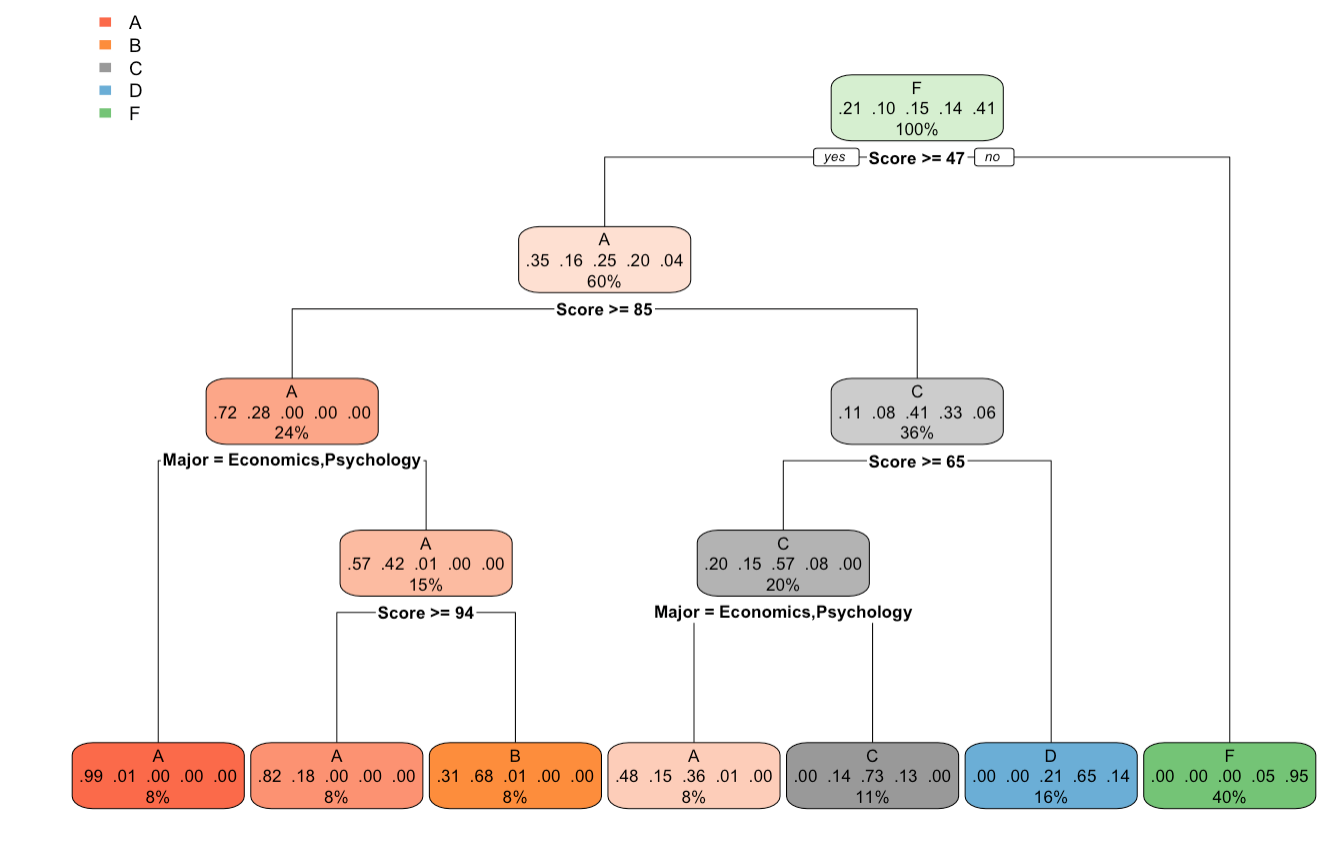
\includegraphics{https://raw.githubusercontent.com/dev7796/data101_tutorial/main/files/img/modeling/2022dt.png}
\caption{Output Plot of \emph{rpart.plot()} function}
\end{figure}

We can see that after plotting the tree using rpart.plot() function, the tree is more readable and provides better information about the splitting conditions, and the probability of outcomes. Each leaf node has information about

\begin{itemize}
\tightlist
\item
  the grade category.
\item
  the outcome probability of each grade category.
\item
  the records percentage out of total records.
\end{itemize}

To study more in detail the arguments that can be passed to the rpart.plot() function, please look at these guides \href{https://www.rdocumentation.org/packages/rpart.plot/versions/3.0.9/topics/rpart.plot}{rpart.plot} and \href{http://www.milbo.org/doc/prp.pdf}{Plotting with rpart.plot (PDF)}

\begin{longtable}[]{@{}l@{}}
\toprule
\endhead
\textbf{NOTE}: In this chapter, from this point forward, the rpart.plots() generated in any example below will be shown as images, and also the code to generate those rpart.plots will be commented in the interactive code blocks. If you want to generate these plots yourself, please use a local Rstudio or R environment. \\
\bottomrule
\end{longtable}

\hypertarget{rpartcontrol}{%
\subsection{Rpart Control}\label{rpartcontrol}}

Now let's look at the rpart.control() function used to pass the control parameters to the control argument of the rpart() function.

\begin{itemize}
\tightlist
\item
  \texttt{rpart.control(\ *minsplit*,\ *minbucket*,\ *cp*,...)}
\item
  \emph{minsplit}: the minimum number of observations that must exist in a node in order for a split to be attempted. For example, minsplit=500 -\textgreater{} the minimum number of observations in a node must be 500 or up, in order to perform the split at the testing condition.
\item
  \emph{minbucket}: minimum number of observations in any terminal(leaf) node. For example, minbucket=500 -\textgreater{} the minimum number of observation in the terminal/leaf node of the trees must be 500 or above.\\
\item
  \emph{cp}: complexity parameter. Using this informs the program that any split which does not increase the accuracy of the fit by \emph{cp}, will not be made in the tree.
\end{itemize}

For more information of the other arguments of the \texttt{rpart.control()} function visit \href{https://www.rdocumentation.org/packages/rpart/versions/4.1-15/topics/rpart.control}{rpart.control}

Let look at few examples.

Suppose you want to set the control parameter minsplit=200.

\hypertarget{snippet-3-minsplit-200}{%
\subsubsection{Snippet 3: Minsplit = 200}\label{snippet-3-minsplit-200}}

eyJsYW5ndWFnZSI6InIiLCJzYW1wbGUiOiJsaWJyYXJ5KHJwYXJ0KVxubW9vZHk8LXJlYWQuY3N2KCdodHRwczovL3Jhdy5naXRodWJ1c2VyY29udGVudC5jb20vZGV2Nzc5Ni9kYXRhMTAxX3R1dG9yaWFsL21haW4vZmlsZXMvZGF0YXNldC9tb29keTIwMjJfbmV3LmNzdicpXG5cbiMgVXNlIG9mIHRoZSBycGFydCgpIGZ1bmN0aW9uIHdpdGggdGhlIGNvbnRyb2wgcGFyYW1ldGVyIG1pbnNwbGl0PTIwMFxudHJlZSA8LSBycGFydChHUkFERSB+IFNDT1JFK0RPWkVTX09GRitURVhUSU5HX0lOX0NMQVNTK1BBUlRJQ0lQQVRJT04sIGRhdGEgPSBtb29keSwgbWV0aG9kID0gXCJjbGFzc1wiLGNvbnRyb2w9cnBhcnQuY29udHJvbChtaW5zcGxpdCA9IDIwMCkpXG5cbnRyZWVcblxuI2xpYnJhcnkocnBhcnQucGxvdClcbiNycGFydC5wbG90KHRyZWUsZXh0cmEgPSAyKSJ9

\begin{figure}
\centering
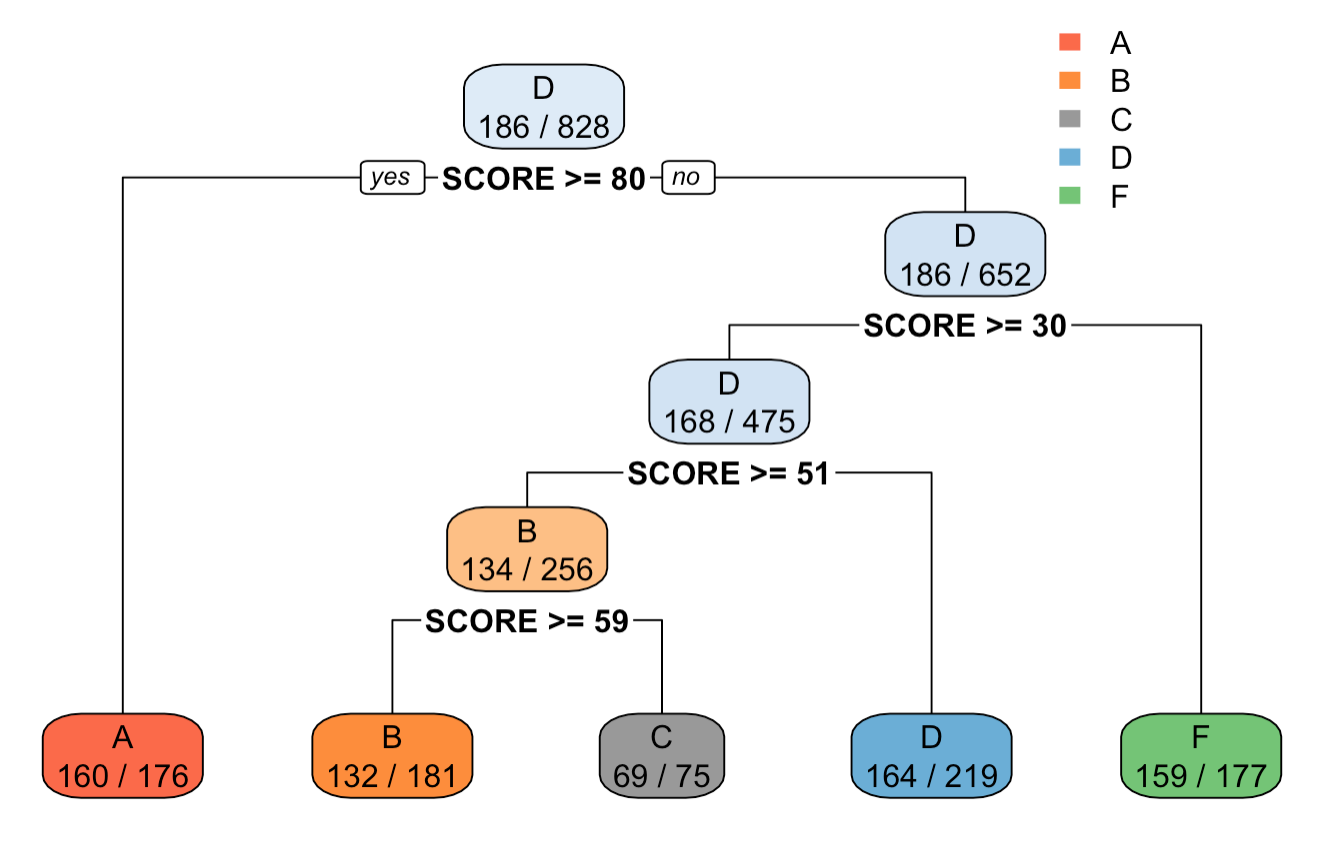
\includegraphics{https://raw.githubusercontent.com/dev7796/data101_tutorial/main/files/img/modeling/2022dt2.png}
\caption{Output tree plot of after setting minsplit=200 in rpart.control() function}
\end{figure}

\hypertarget{snippet-4-minsplit-100}{%
\subsubsection{Snippet 4: Minsplit = 100}\label{snippet-4-minsplit-100}}

eyJsYW5ndWFnZSI6InIiLCJzYW1wbGUiOiJsaWJyYXJ5KHJwYXJ0KVxubW9vZHk8LXJlYWQuY3N2KCdodHRwczovL3Jhdy5naXRodWJ1c2VyY29udGVudC5jb20vZGV2Nzc5Ni9kYXRhMTAxX3R1dG9yaWFsL21haW4vZmlsZXMvZGF0YXNldC9tb29keTIwMjJfbmV3LmNzdicpXG5cbiMgVXNlIG9mIHRoZSBycGFydCgpIGZ1bmN0aW9uIHdpdGggdGhlIGNvbnRyb2wgcGFyYW1ldGVyIG1pbnNwbGl0PTEwMFxudHJlZSA8LSBycGFydChHUkFERSB+IFNDT1JFK0RPWkVTX09GRitURVhUSU5HX0lOX0NMQVNTK1BBUlRJQ0lQQVRJT04sIGRhdGEgPSBtb29keSwgbWV0aG9kID0gXCJjbGFzc1wiLGNvbnRyb2w9cnBhcnQuY29udHJvbChtaW5zcGxpdCA9IDEwMCkpXG5cbnRyZWVcblxuI2xpYnJhcnkocnBhcnQucGxvdClcbiNycGFydC5wbG90KHRyZWUsZXh0cmEgPSAyKSJ9

\begin{figure}
\centering
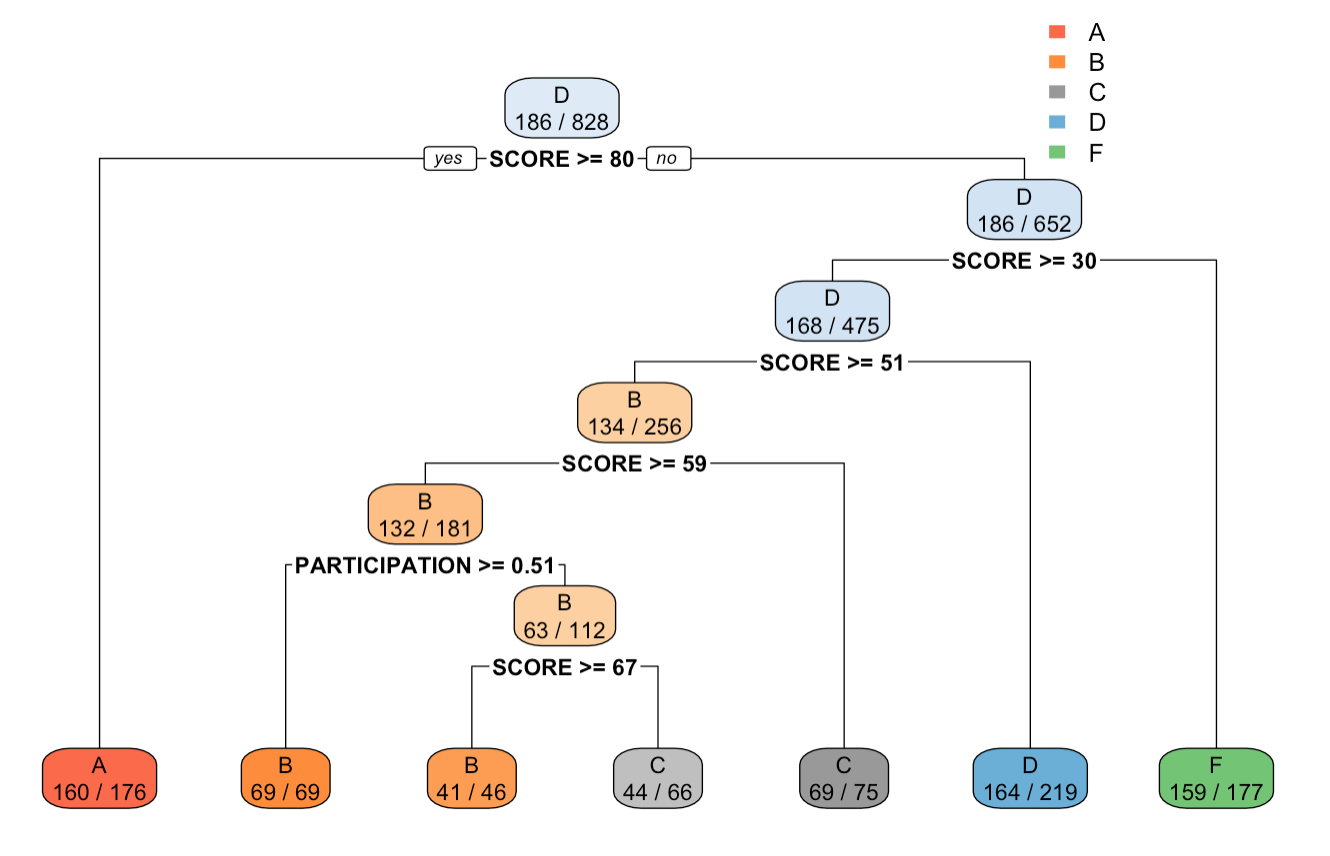
\includegraphics{https://raw.githubusercontent.com/dev7796/data101_tutorial/main/files/img/modeling/2022dt8.png}
\caption{Output tree plot of after setting minsplit=100 in rpart.control() function}
\end{figure}

We can see from the output of \texttt{tree\$splits} and the tree plot, that at each split the total amount of observations are above 200 and 100. Also, in comparison to the tree without control, the tree with control has lower height, and lesser count of splits.

Now, lets set the minbucket parameter to 100, and see how that affects the tree parameters.

\hypertarget{snippet-5-minbucket-100}{%
\subsubsection{Snippet 5: Minbucket = 100}\label{snippet-5-minbucket-100}}

eyJsYW5ndWFnZSI6InIiLCJzYW1wbGUiOiJsaWJyYXJ5KHJwYXJ0KVxubW9vZHk8LXJlYWQuY3N2KCdodHRwczovL3Jhdy5naXRodWJ1c2VyY29udGVudC5jb20vZGV2Nzc5Ni9kYXRhMTAxX3R1dG9yaWFsL21haW4vZmlsZXMvZGF0YXNldC9tb29keTIwMjJfbmV3LmNzdicpXG5cbiMgVXNlIG9mIHRoZSBycGFydCgpIGZ1bmN0aW9uIHdpdGggdGhlIGNvbnRyb2wgcGFyYW1ldGVyIE1pbmJ1Y2tldD0xMDBcbnRyZWUgPC0gcnBhcnQoR1JBREUgfiBTQ09SRStET1pFU19PRkYrVEVYVElOR19JTl9DTEFTUytQQVJUSUNJUEFUSU9OLCBkYXRhID0gbW9vZHksIG1ldGhvZCA9IFwiY2xhc3NcIixjb250cm9sPXJwYXJ0LmNvbnRyb2wobWluYnVja2V0ID0gMTAwKSlcblxudHJlZVxuXG4jbGlicmFyeShycGFydC5wbG90KVxuI3JwYXJ0LnBsb3QodHJlZSxleHRyYSA9IDIpIn0=

\begin{figure}
\centering
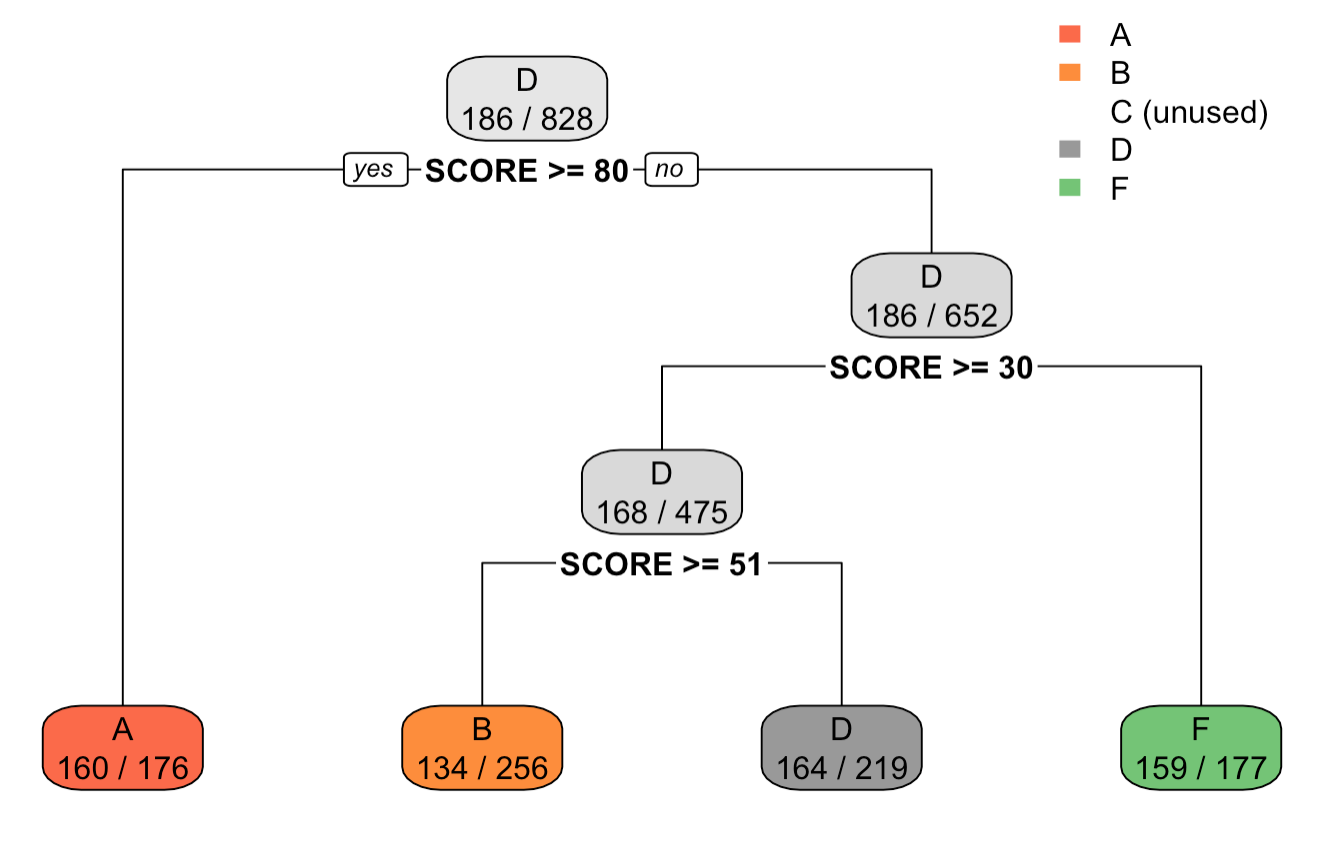
\includegraphics{https://raw.githubusercontent.com/dev7796/data101_tutorial/main/files/img/modeling/2022dt3.png}
\caption{Output tree plot of after setting minbucket=100 in rpart.control() function}
\end{figure}

We can see for the output and the tree plot, that the count of observations in each leaf node is greater than 100. Also, the tree height has shortened, suggesting that the control method was able to shorten the tree size.

\hypertarget{snippet-6-minbucket-200}{%
\subsubsection{Snippet 6: Minbucket = 200}\label{snippet-6-minbucket-200}}

eyJsYW5ndWFnZSI6InIiLCJzYW1wbGUiOiJsaWJyYXJ5KHJwYXJ0KVxubW9vZHk8LXJlYWQuY3N2KCdodHRwczovL3Jhdy5naXRodWJ1c2VyY29udGVudC5jb20vZGV2Nzc5Ni9kYXRhMTAxX3R1dG9yaWFsL21haW4vZmlsZXMvZGF0YXNldC9tb29keTIwMjJfbmV3LmNzdicpXG5cbiMgVXNlIG9mIHRoZSBycGFydCgpIGZ1bmN0aW9uIHdpdGggdGhlIGNvbnRyb2wgcGFyYW1ldGVyIE1pbmJ1Y2tldD0yMDBcbnRyZWUgPC0gcnBhcnQoR1JBREUgfiBTQ09SRStET1pFU19PRkYrVEVYVElOR19JTl9DTEFTUytQQVJUSUNJUEFUSU9OLCBkYXRhID0gbW9vZHksIG1ldGhvZCA9IFwiY2xhc3NcIixjb250cm9sPXJwYXJ0LmNvbnRyb2wobWluYnVja2V0ID0gMjAwKSlcblxudHJlZVxuXG4jbGlicmFyeShycGFydC5wbG90KVxuI3JwYXJ0LnBsb3QodHJlZSxleHRyYSA9IDIpIn0=

\begin{figure}
\centering
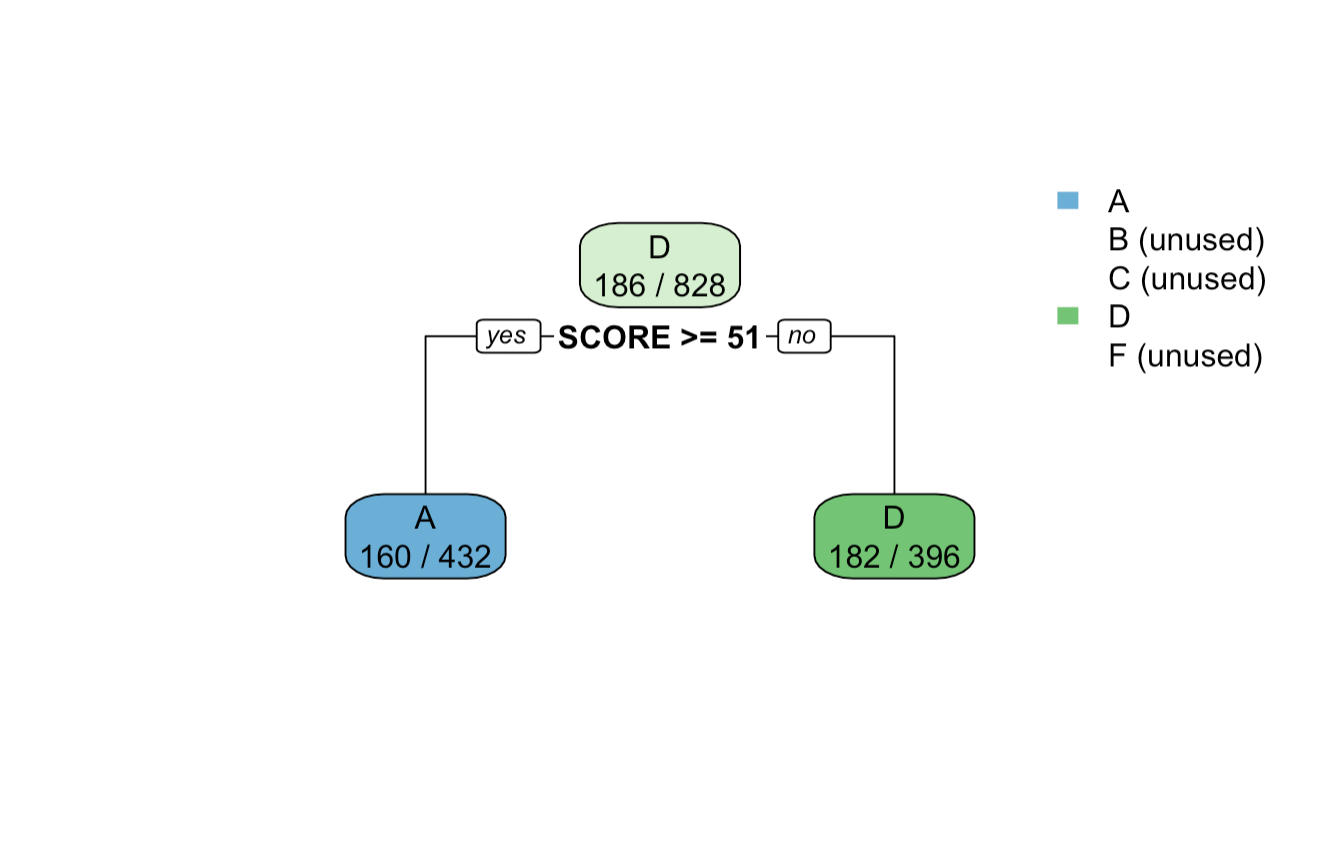
\includegraphics{https://raw.githubusercontent.com/dev7796/data101_tutorial/main/files/img/modeling/2022dt4.png}
\caption{Output tree plot of after setting minbucket=200 in rpart.control() function}
\end{figure}

We can see for the output and the tree plot, that the count of observations in each leaf node is greater than 200. Also, the tree height has shortened, suggesting that the control method was able to shorten the tree size.

Lets now use the \texttt{cp} parameter and see its effect on the tree.

\hypertarget{snippet-7-cp-0.05}{%
\subsubsection{Snippet 7: cp = 0.05}\label{snippet-7-cp-0.05}}

eyJsYW5ndWFnZSI6InIiLCJzYW1wbGUiOiJsaWJyYXJ5KHJwYXJ0KVxubW9vZHk8LXJlYWQuY3N2KCdodHRwczovL3Jhdy5naXRodWJ1c2VyY29udGVudC5jb20vZGV2Nzc5Ni9kYXRhMTAxX3R1dG9yaWFsL21haW4vZmlsZXMvZGF0YXNldC9tb29keTIwMjJfbmV3LmNzdicpXG5cbiMgVXNlIG9mIHRoZSBycGFydCgpIGZ1bmN0aW9uIHdpdGggdGhlIGNvbnRyb2wgcGFyYW1ldGVyIGNwPTAuMlxudHJlZSA8LSBycGFydChHUkFERSB+IC4sIGRhdGEgPSBtb29keSxtZXRob2QgPSBcImNsYXNzXCIsY29udHJvbD1ycGFydC5jb250cm9sKGNwID0gMC4wNSkpXG5cbnRyZWVcblxuI2xpYnJhcnkocnBhcnQucGxvdClcbiNycGFydC5wbG90KHRyZWUpIn0=

\begin{figure}
\centering
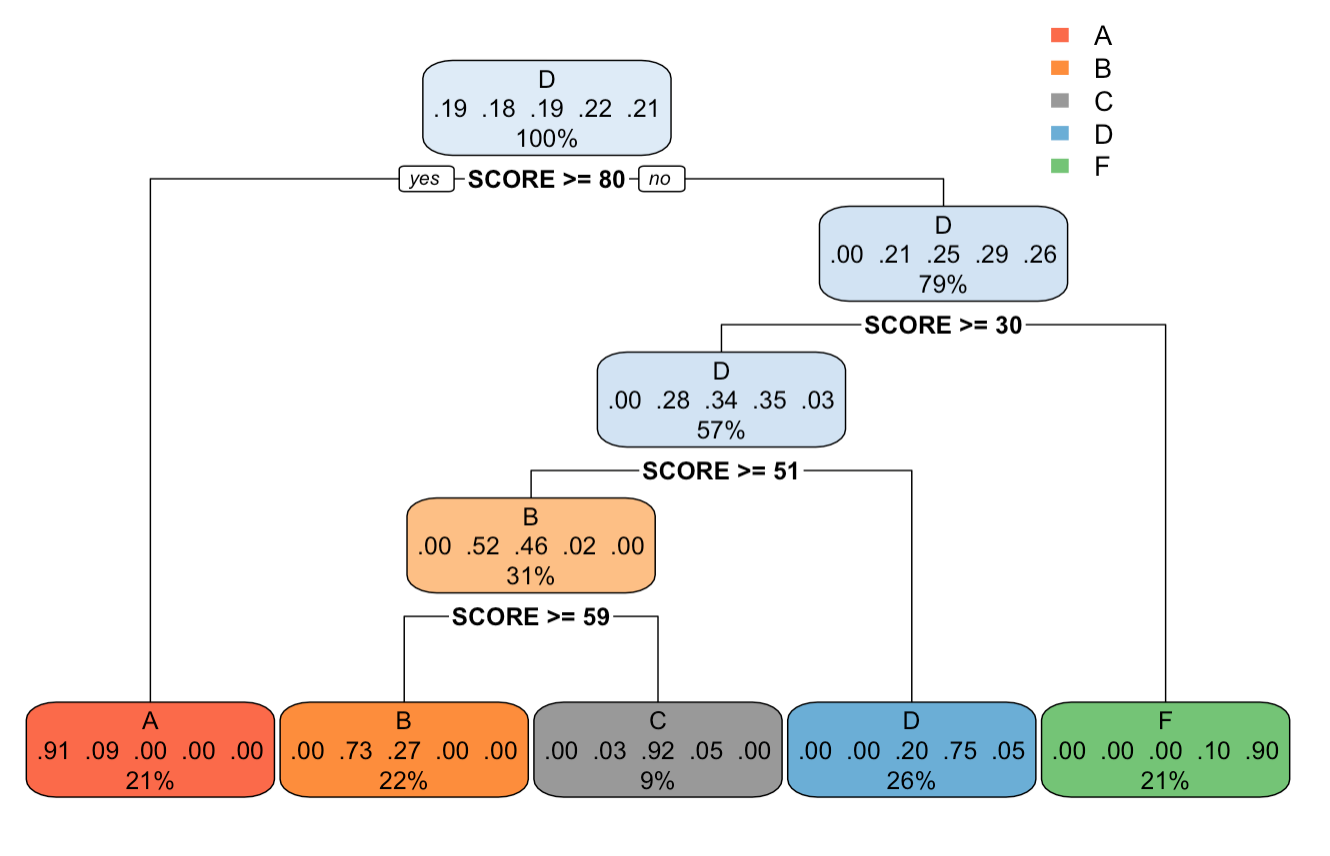
\includegraphics{https://raw.githubusercontent.com/dev7796/data101_tutorial/main/files/img/modeling/2022dt6.png}
\caption{Output tree plot of after setting cp=0.05 in rpart.control() function}
\end{figure}

\hypertarget{snippet-8-cp-0.005}{%
\subsubsection{Snippet 8: cp = 0.005}\label{snippet-8-cp-0.005}}

eyJsYW5ndWFnZSI6InIiLCJzYW1wbGUiOiJsaWJyYXJ5KHJwYXJ0KVxubW9vZHk8LXJlYWQuY3N2KCdodHRwczovL3Jhdy5naXRodWJ1c2VyY29udGVudC5jb20vZGV2Nzc5Ni9kYXRhMTAxX3R1dG9yaWFsL21haW4vZmlsZXMvZGF0YXNldC9tb29keTIwMjJfbmV3LmNzdicpXG5cbiMgVXNlIG9mIHRoZSBycGFydCgpIGZ1bmN0aW9uIHdpdGggdGhlIGNvbnRyb2wgcGFyYW1ldGVyIGNwPTAuMDA1XG50cmVlIDwtIHJwYXJ0KEdSQURFIH4gLiwgZGF0YSA9IG1vb2R5LG1ldGhvZCA9IFwiY2xhc3NcIixjb250cm9sPXJwYXJ0LmNvbnRyb2woY3AgPSAwLjAwNSkpXG5cbnRyZWVcblxuI2xpYnJhcnkocnBhcnQucGxvdClcbiNycGFydC5wbG90KHRyZWUpIn0=

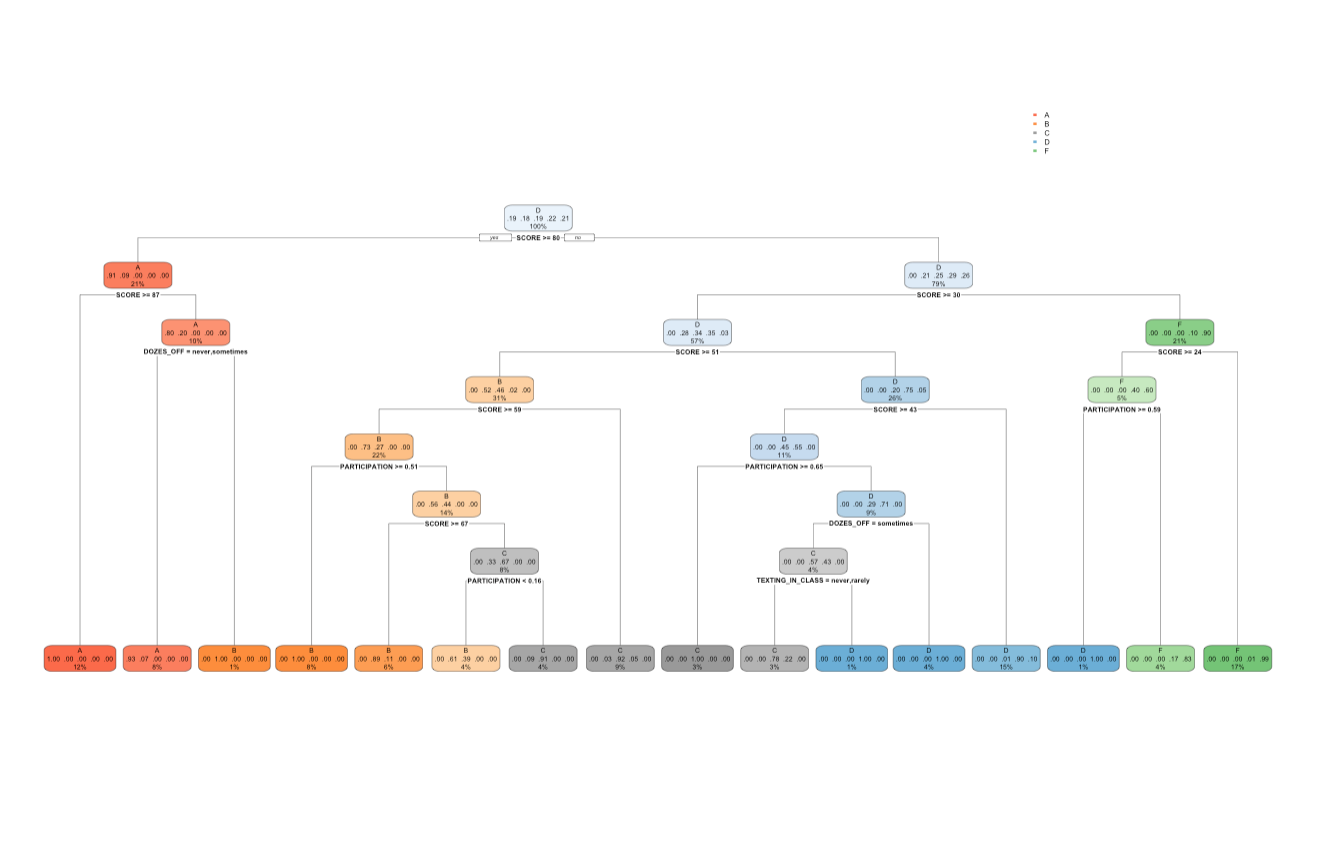
\includegraphics{https://raw.githubusercontent.com/dev7796/data101_tutorial/main/files/img/modeling/2022dt7.png}
We can see for the output and the tree plot, that the tree size has increased, with increase in number of splits, and leaf nodes. Also we can see that the minimum CP value in the output is 0.005.

\hypertarget{crossvalidation}{%
\subsection{Cross Validation}\label{crossvalidation}}

Overfitting takes place when you have a high accuracy on training dataset, but a low accuracy on the test dataset. But how do you know whether you are overfitting or not? Especially since you cannot determine accuracy on the test dataset? That is where cross-validation comes into play.

Because we cannot determine accuracy on test dataset, we partition our training dataset into train and validation (testing). We train our model (rpart or lm) on train partition and test on the validation partition. The partition is defined by split ratio. If split ratio =0.7, 70\% of the training dataset will be used for the actual training of your model (rpart or lm), and 30 \% will be used for validation (or testing). The accuracy of this validation data is called cross-validation accuracy.

To know if you are overfitting or not, compare the training accuracy with the cross-validation accuracy. If your training accuracy is high, and cross-validation accuracy is low, that means you are overfitting.

\begin{itemize}
\tightlist
\item
  \texttt{cross\_validate(*data*,\ *tree*,\ *n\_iter*,\ *split\_ratio*,\ *method*)}

  \begin{itemize}
  \tightlist
  \item
    \emph{data}: The dataset on which cross validation is to be performed.
  \item
    \emph{tree}: The decision tree generated using rpart.
  \item
    \emph{n\_iter}: Number of iterations.
  \item
    \emph{split\_ratio}: The splitting ratio of the data into train data and validation data.
  \item
    \emph{method}: Method of the prediction. ``class'' for classification.
  \end{itemize}
\end{itemize}

The way the function works is as follows:

\begin{itemize}
\tightlist
\item
  It randomly partitions your data into training and validation.
\item
  It then constructs the following two decision trees on training partition:

  \begin{itemize}
  \tightlist
  \item
    The tree that you pass to the function.
  \item
    The tree is constructed on all attributes as predictors and with no control parameters.
    -It then determines the accuracy of the two trees on validation partition and returns you the accuracy values for both the trees.
  \end{itemize}
\end{itemize}

The values in the first column(accuracy\_subset) returned by cross-validation function are more important when it comes to detecting overfitting. If these values are much lower than the training accuracy you get, that means you are overfitting.

We would also want the values in accuracy\_subset to be close to each other (in other words, have low variance). If the values are quite different from each other, that means your model (or tree) has a high variance which is not desired.

The second column(accuracy\_all) tells you what happens if you construct a tree based on all attributes. If these values are larger than accuracy\_subset, that means you are probably leaving out attributes from your tree that are relevant.

Each iteration of cross-validation creates a different random partition of train and validation, and so you have possibly different accuracy values for every iteration.

Let's look at the cross\_validate() function in action in the example below.

We will pass the tree with formula as \texttt{GRADE\ \textasciitilde{}\ SCORE+DOZES\_OFF+TEXTING\_IN\_CLASS+PARTICIPATION}, and control parameter, with \texttt{minsplit=100}.
And for cross\_validate() function, we will use\texttt{n\_iter=5,\ and\ split\_raitio=0.7}

\begin{longtable}[]{@{}l@{}}
\toprule
\endhead
\textbf{NOTE:} Cross-Validation repository is already preloaded for the following interactive code block. Thus you can directly use the cross\_validate() function in the following interactive code block. But if you wish to use the code\_validate() function locally, please use \\
\bottomrule
\end{longtable}

\begin{verbatim}
install.packages("devtools") 
devtools::install_github("devanshagr/CrossValidation")
CrossValidation::cross_validate()
\end{verbatim}

\hypertarget{snippet-9}{%
\subsubsection{Snippet 9}\label{snippet-9}}

eyJsYW5ndWFnZSI6InIiLCJwcmVfZXhlcmNpc2VfY29kZSI6ImNyb3NzX3ZhbGlkYXRlIDwtIGZ1bmN0aW9uKGRmLCB0cmVlLCBuX2l0ZXIsIHNwbGl0X3JhdGlvLCBtZXRob2QgPSAnY2xhc3MnKVxue1xuICAjIHRyYWluaW5nIGRhdGEgZnJhbWUgZGZcbiAgZGYgPC0gYXMuZGF0YS5mcmFtZShkZilcblxuICAjIG1lYW5fc3Vic2V0IGlzIGEgdmVjdG9yIG9mIGFjY3VyYWN5IHZhbHVlcyBnZW5lcmF0ZWQgZnJvbSB0aGUgc3BlY2lmaWVkIGZlYXR1cmVzIGluIHRoZSB0cmVlIG9iamVjdFxuICBtZWFuX3N1YnNldCA8LSBjKClcblxuICAjIG1lYW5fYWxsIGlzIGEgdmVjdG9yIG9mIGFjY3VyYWN5IHZhbHVlcyBnZW5lcmF0ZWQgZnJvbSBhbGwgdGhlIGF2YWlsYWJsZSBmZWF0dXJlcyBpbiB0aGUgZGF0YSBmcmFtZVxuICBtZWFuX2FsbCA8LSBjKClcblxuICAjIGNvbnRyb2wgcGFyYW1ldGVycyBmb3IgdGhlIGRlY2lzaW9uIHRyZWVcbiAgY29udHJvID0gdHJlZSRjb250cm9sXG5cbiAgIyB0aGUgZm9sbG93aW5nIHNuaXBwZXQgd2lsbCBjcmVhdGUgcmVsYXRpb25zIHRvIGdlbmVyYXRlIGRlY2lzaW9uIHRyZWVzXG4gICMgcmVsYXRpb25fYWxsIHdpbGwgY3JlYXRlIGEgZGVjaXNpb24gdHJlZSB3aXRoIGFsbCB0aGUgZmVhdHVyZXNcbiAgIyByZWxhdGlvbl9zdWJzZXQgd2lsbCBjcmVhdGUgYSBkZWNpc2lvbiB0cmVlIHdpdGggb25seSB1c2VyLXNwZWNpZmllZCBmZWF0dXJlcyBpbiB0cmVlXG4gIGRlcCA8LSBhbGwudmFycyh0ZXJtcyh0cmVlKSlbMV1cbiAgaW5kZXAgPC0gbGlzdCgpXG4gIHJlbGF0aW9uX2FsbCA9IGFzLmZvcm11bGEocGFzdGUoZGVwLCAnLicsIHNlcCA9IFwiflwiKSlcbiAgaSA8LSAxXG4gIHdoaWxlIChpIDwgbGVuZ3RoKGFsbC52YXJzKHRlcm1zKHRyZWUpKSkpIHtcbiAgICBpbmRlcFtbaV1dIDwtIGFsbC52YXJzKHRlcm1zKHRyZWUpKVtpICsgMV1cbiAgICBpIDwtIGkgKyAxXG4gIH1cbiAgYiA8LSBwYXN0ZShpbmRlcCwgY29sbGFwc2UgPSBcIitcIilcbiAgcmVsYXRpb25fc3Vic2V0IDwtIGFzLmZvcm11bGEocGFzdGUoZGVwLCBiLCBzZXAgPSBcIn5cIikpXG5cbiAgIyBjcmVhdGluZyB0cmFpbiBhbmQgdGVzdCBzYW1wbGVzIHdpdGggdGhlIGdpdmVuIHNwbGl0IHJhdGlvXG4gICMgcGVyZm9ybWluZyBjcm9zcy12YWxpZGF0aW9uIG5faXRlciB0aW1lc1xuICBmb3IgKGkgaW4gMTpuX2l0ZXIpIHtcbiAgICBzYW1wbGUgPC1cbiAgICAgIHNhbXBsZS5pbnQobiA9IG5yb3coZGYpLFxuICAgICAgICAgICAgICAgICBzaXplID0gZmxvb3Ioc3BsaXRfcmF0aW8gKiBucm93KGRmKSksXG4gICAgICAgICAgICAgICAgIHJlcGxhY2UgPSBGKVxuICAgIHRyYWluIDwtIGRmW3NhbXBsZSxdXG4gICAgdGVzdGluZyAgPC0gZGZbLXNhbXBsZSxdXG4gICAgdHlwZSA9IHR5cGVvZih1bmxpc3QodGVzdGluZ1tkZXBdKSlcblxuICAgICMgZGVjaXNpb24gdHJlZSBmb3IgcmVncmVzc2lvbiBpZiB0aGUgbWV0aG9kIHNwZWNpZmllZCBpcyBcImFub3ZhXCJcbiAgICBpZiAobWV0aG9kID09ICdhbm92YScpIHtcbiAgICAgIGZpcnN0LnRyZWUgPC1cbiAgICAgICAgcnBhcnQoXG4gICAgICAgICAgcmVsYXRpb25fc3Vic2V0LFxuICAgICAgICAgIGRhdGEgPSB0cmFpbixcbiAgICAgICAgICBjb250cm9sID0gY29udHJvLFxuICAgICAgICAgIG1ldGhvZCA9ICdhbm92YSdcbiAgICAgICAgKVxuICAgICAgc2Vjb25kLnRyZWUgPC0gcnBhcnQocmVsYXRpb25fYWxsLCBkYXRhID0gdHJhaW4sIG1ldGhvZCA9ICdhbm92YScpXG4gICAgICBwcmVkMS50cmVlIDwtIHByZWRpY3QoZmlyc3QudHJlZSwgbmV3ZGF0YSA9IHRlc3RpbmcpXG4gICAgICBwcmVkMi50cmVlIDwtIHByZWRpY3Qoc2Vjb25kLnRyZWUsIG5ld2RhdGEgPSB0ZXN0aW5nKVxuICAgICAgbWVhbjEgPC0gbWVhbigoYXMubnVtZXJpYyhwcmVkMS50cmVlKSAtIHRlc3RpbmdbLCBkZXBdKSBeIDIpXG4gICAgICBtZWFuMiA8LSBtZWFuKChhcy5udW1lcmljKHByZWQyLnRyZWUpIC0gdGVzdGluZ1ssIGRlcF0pIF4gMilcbiAgICAgIG1lYW5fc3Vic2V0IDwtIGMobWVhbl9zdWJzZXQsIG1lYW4xKVxuICAgICAgbWVhbl9hbGwgPC0gYyhtZWFuX2FsbCwgbWVhbjIpXG4gICAgfVxuXG4gICAgIyBkZWNpc2lvbiB0cmVlIGZvciBjbGFzc2lmaWNhdGlvblxuICAgICMgaWYgdGhlIG1ldGhvZCBzcGVjaWZpZWQgaXMgbm90IFwiYW5vdmFcIiwgdGhlbiB0aGlzIGJsb2NrIGlzIGV4ZWN1dGVkXG4gICAgIyBpZiB0aGUgbWV0aG9kIGlzIG5vdCBzcGVjaWZpZWQgYnkgdGhlIHVzZXIsIHRoZSBkZWZhdWx0IG9wdGlvbiBpcyB0byBwZXJmb3JtIGNsYXNzaWZpY2F0aW9uXG4gICAgZWxzZXtcbiAgICAgIGZpcnN0LnRyZWUgPC1cbiAgICAgICAgcnBhcnQoXG4gICAgICAgICAgcmVsYXRpb25fc3Vic2V0LFxuICAgICAgICAgIGRhdGEgPSB0cmFpbixcbiAgICAgICAgICBjb250cm9sID0gY29udHJvLFxuICAgICAgICAgIG1ldGhvZCA9ICdjbGFzcydcbiAgICAgICAgKVxuICAgICAgc2Vjb25kLnRyZWUgPC0gcnBhcnQocmVsYXRpb25fYWxsLCBkYXRhID0gdHJhaW4sIG1ldGhvZCA9ICdjbGFzcycpXG4gICAgICBwcmVkMS50cmVlIDwtIHByZWRpY3QoZmlyc3QudHJlZSwgbmV3ZGF0YSA9IHRlc3RpbmcsIHR5cGUgPSAnY2xhc3MnKVxuICAgICAgcHJlZDIudHJlZSA8LVxuICAgICAgICBwcmVkaWN0KHNlY29uZC50cmVlLCBuZXdkYXRhID0gdGVzdGluZywgdHlwZSA9ICdjbGFzcycpXG4gICAgICBtZWFuMSA8LVxuICAgICAgICBtZWFuKGFzLmNoYXJhY3RlcihwcmVkMS50cmVlKSA9PSBhcy5jaGFyYWN0ZXIodGVzdGluZ1ssIGRlcF0pKVxuICAgICAgbWVhbjIgPC1cbiAgICAgICAgbWVhbihhcy5jaGFyYWN0ZXIocHJlZDIudHJlZSkgPT0gYXMuY2hhcmFjdGVyKHRlc3RpbmdbLCBkZXBdKSlcbiAgICAgIG1lYW5fc3Vic2V0IDwtIGMobWVhbl9zdWJzZXQsIG1lYW4xKVxuICAgICAgbWVhbl9hbGwgPC0gYyhtZWFuX2FsbCwgbWVhbjIpXG4gICAgfVxuICB9XG5cbiAgIyBhdmVyYWdlX2FjY3VyYWN5X3N1YnNldCBpcyB0aGUgYXZlcmFnZSBhY2N1cmFjeSBvZiBuX2l0ZXIgaXRlcmF0aW9ucyBvZiBjcm9zcy12YWxpZGF0aW9uIHdpdGggdXNlci1zcGVjaWZpZWQgZmVhdHVyZXNcbiAgIyBhdmVyYWdlX2FjdXJhY3lfYWxsIGlzIHRoZSBhdmVyYWdlIGFjY3VyYWN5IG9mIG5faXRlciBpdGVyYXRpb25zIG9mIGNyb3NzLXZhbGlkYXRpb24gd2l0aCBhbGwgdGhlIGF2YWlsYWJsZSBmZWF0dXJlc1xuICAjIHZhcmlhbmNlX2FjY3VyYWN5X3N1YnNldCBpcyB0aGUgdmFyaWFuY2Ugb2YgYWNjdXJhY3kgb2Ygbl9pdGVyIGl0ZXJhdGlvbnMgb2YgY3Jvc3MtdmFsaWRhdGlvbiB3aXRoIHVzZXItc3BlY2lmaWVkIGZlYXR1cmVzXG4gICMgdmFyaWFuY2VfYWNjdXJhY3lfYWxsIGlzIHRoZSB2YXJpYW5jZSBvZiBhY2N1cmFjeSBvZiBuX2l0ZXIgaXRlcmF0aW9ucyBvZiBjcm9zcy12YWxpZGF0aW9uIHdpdGggYWxsIHRoZSBhdmFpbGFibGUgZmVhdHVyZXNcbiAgY3Jvc3NfdmFsaWRhdGlvbl9zdGF0cyA8LVxuICAgIGxpc3QoXG4gICAgICBcImF2ZXJhZ2VfYWNjdXJhY3lfc3Vic2V0XCIgPSBtZWFuKG1lYW5fc3Vic2V0LCBuYS5ybSA9IFQpLFxuICAgICAgXCJhdmVyYWdlX2FjY3VyYWN5X2FsbFwiID0gbWVhbihtZWFuX2FsbCwgbmEucm0gPSBUKSxcbiAgICAgIFwidmFyaWFuY2VfYWNjdXJhY3lfc3Vic2V0XCIgPSB2YXIobWVhbl9zdWJzZXQsIG5hLnJtID0gVCksXG4gICAgICBcInZhcmlhbmNlX2FjY3VyYWN5X2FsbFwiID0gdmFyKG1lYW5fYWxsLCBuYS5ybSA9IFQpXG4gICAgKVxuXG4gICMgY3JlYXRpbmcgYSBkYXRhIGZyYW1lIG9mIGFjY3VyYWN5X3N1YnNldCBhbmQgYWNjdXJhY3lfYWxsXG4gICMgYWNjdXJhY3lfc3Vic2V0IGNvbnRhaW5zIG5faXRlciBhY2N1cmFjeSB2YWx1ZXMgb24gY3Jvc3MtdmFsaWRhdGlvbiB3aXRoIHVzZXItc3BlY2lmaWVkIGZlYXR1cmVzXG4gICMgYWNjdXJhY3lfYWxsIGNvbnRhaW5zIG5faXRlciBhY2N1cmFjeSB2YWx1ZXMgb24gY3Jvc3MtdmFsaWRhdGlvbiB3aXRoIGFsbCB0aGUgYXZhaWxhYmxlIGZlYXR1cmVzXG4gIGNyb3NzX3ZhbGlkYXRpb25fZGYgPC1cbiAgICBkYXRhLmZyYW1lKGFjY3VyYWN5X3N1YnNldCA9IG1lYW5fc3Vic2V0LCBhY2N1cmFjeV9hbGwgPSBtZWFuX2FsbClcbiAgcmV0dXJuKGxpc3QoY3Jvc3NfdmFsaWRhdGlvbl9kZiwgY3Jvc3NfdmFsaWRhdGlvbl9zdGF0cykpXG59Iiwic2FtcGxlIjoiIyBGaXJzdCBsZXRzIGltcG9ydCB0aGUgcnBhcnQgbGlicmFyeVxubGlicmFyeShycGFydClcbiMgSW1wb3J0IGRhdGFzZXRcbm1vb2R5PC1yZWFkLmNzdignaHR0cHM6Ly9yYXcuZ2l0aHVidXNlcmNvbnRlbnQuY29tL2Rldjc3OTYvZGF0YTEwMV90dXRvcmlhbC9tYWluL2ZpbGVzL2RhdGFzZXQvbW9vZHkyMDIyX25ldy5jc3YnLHN0cmluZ3NBc0ZhY3RvcnMgPSBUKVxuIyBVc2Ugb2YgdGhlIHJwYXJ0KCkgZnVuY3Rpb24uXG50cmVlIDwtIHJwYXJ0KEdSQURFIH4gU0NPUkUrRE9aRVNfT0ZGK1RFWFRJTkdfSU5fQ0xBU1MsIGRhdGEgPSBtb29keSxtZXRob2QgPSBcImNsYXNzXCIsY29udHJvbCA9IHJwYXJ0LmNvbnRyb2wobWluc3BsaXQgPSAxMDApKVxudHJlZVxuIyBOb3cgbGV0cyBwcmVkaWN0IHRoZSBHcmFkZXMgb2YgdGhlIE1vb2R5IERhdGFzZXQuXG5wcmVkIDwtIHByZWRpY3QodHJlZSwgbW9vZHksIHR5cGU9XCJjbGFzc1wiKVxuaGVhZChwcmVkKVxuIyBMZXRzIGNoZWNrIHRoZSBUcmFpbmluZyBBY2N1cmFjeVxubWVhbihtb29keSRHUkFERT09cHJlZClcbiMgTGV0cyB1cyB0aGUgY3Jvc3NfdmFsaWRhdGUoKSBmdW5jdGlvbi5cbmNyb3NzX3ZhbGlkYXRlKG1vb2R5LHRyZWUsNSwwLjcpIn0=

You can see that the cross-validation accuracies for the tree that was passed (accuracy\_subset) are fairly high and close to our training accuracy of 84\%. This means we are not overfitting. Also observe that accuracy\_subset and accuracy\_all have the same values, which means that the only relevant attributes are score and participation, and adding more attributes doesn't make any difference to the tree. Finally, the values in accuracy\_subset are reasonably close to each other, which mean low variance.

\hypertarget{rpartpredict}{%
\subsection{Prediction using rpart.}\label{rpartpredict}}

Now that we have seen the process to create a decision tree and also plot it, we will like to use the output tree to predict the required attribute.

From the moody example, we are trying to predict the grade of students. Lets look at the \texttt{predict()} function to predict the outcomes.

\begin{itemize}
\tightlist
\item
  \texttt{predict(*object*,*data*,*type*,...)}

  \begin{itemize}
  \tightlist
  \item
    \emph{object}: the generated tree from the rpart function.
  \item
    \emph{data}: the data on which the prediction is to be performed.
  \item
    \emph{type}: the type of prediction required. One of ``vector'', ``prob'', ``class'' or ``matrix''.
  \end{itemize}
\end{itemize}

Now lets use the predict function to predict the grades of students using the tree generated on the Moody dataset.

\hypertarget{snippet-10}{%
\subsubsection{Snippet 10}\label{snippet-10}}

eyJsYW5ndWFnZSI6InIiLCJzYW1wbGUiOiIjIEZpcnN0IGxldHMgaW1wb3J0IHRoZSBycGFydCBsaWJyYXJ5XG5saWJyYXJ5KHJwYXJ0KVxuXG4jIEltcG9ydCBkYXRhc2V0XG5tb29keTwtcmVhZC5jc3YoJ2h0dHBzOi8vcmF3LmdpdGh1YnVzZXJjb250ZW50LmNvbS9kZXY3Nzk2L2RhdGExMDFfdHV0b3JpYWwvbWFpbi9maWxlcy9kYXRhc2V0L21vb2R5MjAyMl9uZXcuY3N2JylcblxuIyBVc2Ugb2YgdGhlIHJwYXJ0KCkgZnVuY3Rpb24uXG50cmVlIDwtIHJwYXJ0KEdSQURFIH4gU0NPUkUrRE9aRVNfT0ZGK1RFWFRJTkdfSU5fQ0xBU1MrUEFSVElDSVBBVElPTiwgZGF0YSA9IG1vb2R5ICxtZXRob2QgPSBcImNsYXNzXCIpXG50cmVlXG5cbiMgTm93IGxldHMgcHJlZGljdCB0aGUgR3JhZGVzIG9mIHRoZSBNb29keSBEYXRhc2V0LlxucHJlZCA8LSBwcmVkaWN0KHRyZWUsIG1vb2R5LCB0eXBlPVwiY2xhc3NcIilcbmhlYWQocHJlZCkifQ==

\hypertarget{snippet-11-your-model-with-rpart}{%
\subsection{Snippet 11: Your Model with rpart}\label{snippet-11-your-model-with-rpart}}

eyJsYW5ndWFnZSI6InIiLCJzYW1wbGUiOiIjSG93IHRvIGNvbWJpbmUgeW91ciBmcmVlc3R5bGUgcHJlZGljdGlvbiBtb2RlbCB3aXRoIHRoZSBycGFydD8gXG5cbiNPbmUgd2F5IG9mIGRvaW5nIGl0IGlzIHRvIGRpdmlkZSB0aGUgZGF0YSBzZXRzIGludG8gdHdvIG11dHVhbGx5IGV4Y2x1c2l2ZSBzdWJzZXRzICh3aGljaCBjb3ZlciBhbGwgZGF0YSBhbHNvKS4gIEhvdyBkbyB5b3UgbWFrZSB0aGVzZSBzdWJzZXRzPyAgVW5mb3J0dW5hdGVseSB0aGVyZSBpcyBubyBhbGdvcml0aG0gZm9yIHRoaXMgYW5kIGl0IGlzIG1vcmUgcmVseWluZyBvbiBob3cgd2VsbCBpcyB5b3VyIG1vZGVsIGRvaW5nIGZvciBkaWZmZXJlbnQgc2xpY2VzIG9mIHRoZSBkYXRhLiAgXG5cbiNJbiB0aGlzIGV4YW1wbGUgKHNpbWlsYXJseSB0byBzbmlwcGV0IDE2Ljcgd2hlcmUgd2UgY29tYmluZSB0d28gcnBhcnQgbW9kZWxzLCB3ZSBhc3N1bWUgdGhhdCBpbml0aWFsIHNwbGl0IHdlIGRlY2lkZWQgb24gaXMgYmFzZWQgb24gU0NPUkUuIEJ1dCBpbnN0ZWFkIG9mIGhhdmluZyB0d28gcnBhcnQgbW9kZWxzICAoMTYuNyksIHdlIHdpbGwgdXNlIG91ciBwcmVkaWN0aW9uICBtb2RlbCBmcm9tIHByZWRpY3Rpb24gY2hhbGxlbmdlIDEgIGZvciBTQ09SRSA+NTAgYW5kIHJwYXJ0IGZvciBTQ09SRSA8PTUwLlxuXG4jTGV0cyBhc3N1bWUgdGhhdCB5b3VyUHJlZGljdGlvbiBpcyBvdXIgbW9kZWwgZnJvbSBQcmVkaWN0aW9uIENoYWxsZW5nZSAxICh5b3VyIGVudGlyZSBjb2RlIGhhcyB0byBiZSBhcHBsaWVkIGhlcmUgdG8gdGhlIGRhdGEgc2V0IChtb29keSwgYmVsb3cpXG5cbm1vb2R5PC1yZWFkLmNzdignaHR0cHM6Ly9yYXcuZ2l0aHVidXNlcmNvbnRlbnQuY29tL2Rldjc3OTYvZGF0YTEwMV90dXRvcmlhbC9tYWluL2ZpbGVzL2RhdGFzZXQvbW9vZHkyMDIyX25ldy5jc3YnKVxuXG4jcnBhcnRNb2RlbDwtcnBhcnQoR1JBREV+LiwgZGF0YT1tb29keVttb29keSRTQ09SRTw9NTAsXSk7XG4jcHJlZF9ycGFydE1vZGVsIDwtIHByZWRpY3QocnBhcnRNb2RlbCwgbmV3ZGF0YT1tb29keVttb29keSRTQ09SRTw9NTAsXSwgdHlwZT1cImNsYXNzXCIpXG4jcHJlZF95b3VyTW9kZWwgPC0geW91clByZWRpY3Rpb25bbW9vZHkkU0NPUkU8PTUwXVxuI215cHJlZGljdGlvbjwtbW9vZHlcblxuIyMgSGVyZSB3ZSBjb21iaW5lIHR3byBtb2RlbHMgLSBvdXIgbW9kZWwgZnJvbSBwcmVkaWN0aW9uIDEgY2hhbGxlbmdlIGFuZCBycGFydC5cblxuI2RlY2lzaW9uIDwtIHJlcCgnRicsbnJvdyhteXByZWRpY3Rpb24pKVxuI2RlY2lzaW9uW215cHJlZGljdGlvbiRTQ09SRT41MF0gPC0gcHJlZF95b3VyTW9kZWxcbiNkZWNpc2lvbltteXByZWRpY3Rpb24kU0NPUkU8PTUwXSA8LWFzLmNoYXJhY3RlcihwcmVkX3JwYXJ0TW9kZWwgKVxuI215cHJlZGljdGlvbiRHUkFERSA8LWRlY2lzaW9uXG4jZXJyb3IgPC0gbWVhbihtb29keSRHUkFERSE9IG15cHJlZGljdGlvbiRHUkFERVxuI2Vycm9yIn0=

\hypertarget{snippet-12-freestyle-rpart-combining-rpart-prediction-models}{%
\subsection{Snippet 12: Freestyle + rpart: Combining rpart prediction models}\label{snippet-12-freestyle-rpart-combining-rpart-prediction-models}}

eyJsYW5ndWFnZSI6InIiLCJzYW1wbGUiOiJsaWJyYXJ5KHJwYXJ0KVxuIyBJbXBvcnQgZGF0YXNldFxubW9vZHk8LXJlYWQuY3N2KCdodHRwczovL3Jhdy5naXRodWJ1c2VyY29udGVudC5jb20vZGV2Nzc5Ni9kYXRhMTAxX3R1dG9yaWFsL21haW4vZmlsZXMvZGF0YXNldC9tb29keTIwMjJfbmV3LmNzdicpXG5tb2RlbDE8LXJwYXJ0KEdSQURFfi4sIGRhdGE9bW9vZHlbbW9vZHkkU0NPUkU+NTAsXSk7XG5tb2RlbDI8LXJwYXJ0KEdSQURFfi4sIGRhdGE9bW9vZHlbbW9vZHkkU0NPUkU8PTUwLF0pO1xubW9kZWwxXG5tb2RlbDJcbnByZWQxIDwtIHByZWRpY3QobW9kZWwxLCBuZXdkYXRhPW1vb2R5W21vb2R5JFNDT1JFPjUwLF0sIHR5cGU9XCJjbGFzc1wiKVxucHJlZDIgPC0gcHJlZGljdChtb2RlbDIsIG5ld2RhdGE9bW9vZHlbbW9vZHkkU0NPUkU8PTUwLF0sIHR5cGU9XCJjbGFzc1wiKVxubXlwcmVkaWN0aW9uPC1tb29keVxuZGVjaXNpb24gPC0gcmVwKCdGJyxucm93KG15cHJlZGljdGlvbikpXG5kZWNpc2lvbltteXByZWRpY3Rpb24kU0NPUkU+NTBdIDwtIGFzLmNoYXJhY3RlcihwcmVkMSlcbmRlY2lzaW9uW215cHJlZGljdGlvbiRTQ09SRTw9NTBdIDwtYXMuY2hhcmFjdGVyKHByZWQyKVxubXlwcmVkaWN0aW9uJEdSQURFIDwtZGVjaXNpb25cbmVycm9yIDwtIG1lYW4obW9vZHkkR1JBREUhPSBteXByZWRpY3Rpb24kR1JBREUpXG5lcnJvciJ9

\hypertarget{snippet-13-submission-with-rpart}{%
\subsection{Snippet 13: Submission with rpart}\label{snippet-13-submission-with-rpart}}

eyJsYW5ndWFnZSI6InIiLCJzYW1wbGUiOiJsaWJyYXJ5KHJwYXJ0KVxudGVzdDwtcmVhZC5jc3YoJ2h0dHBzOi8vcmF3LmdpdGh1YnVzZXJjb250ZW50LmNvbS9kZXY3Nzk2L2RhdGExMDFfdHV0b3JpYWwvbWFpbi9maWxlcy9kYXRhc2V0L00yMDIydGVzdFNOb0dyYWRlLmNzdicpXG5zdWJtaXNzaW9uPC1yZWFkLmNzdignaHR0cHM6Ly9yYXcuZ2l0aHVidXNlcmNvbnRlbnQuY29tL2Rldjc3OTYvZGF0YTEwMV90dXRvcmlhbC9tYWluL2ZpbGVzL2RhdGFzZXQvTTIwMjJzdWJtaXNzaW9uLmNzdicpXG50cmFpbiA8LSByZWFkLmNzdihcImh0dHBzOi8vcmF3LmdpdGh1YnVzZXJjb250ZW50LmNvbS9kZXY3Nzk2L2RhdGExMDFfdHV0b3JpYWwvbWFpbi9maWxlcy9kYXRhc2V0L00yMDIydHJhaW4uY3N2XCIpXG5cbnRyZWUgPC0gcnBhcnQoR3JhZGUgfiBNYWpvcitTY29yZStTZW5pb3JpdHksIGRhdGEgPSB0cmFpbiwgbWV0aG9kID0gXCJjbGFzc1wiLGNvbnRyb2w9cnBhcnQuY29udHJvbChtaW5idWNrZXQgPSAyMDApKVxudHJlZVxuXG5wcmVkaWN0aW9uIDwtIHByZWRpY3QodHJlZSwgdGVzdCwgdHlwZT1cImNsYXNzXCIpXG5cbiNOb3cgbWFrZSB5b3VyIHN1Ym1pc3Npb24gZmlsZSAtIGl0IHdpbGwgaGF2ZSB0aGUgSURzIGFuZCBub3cgdGhlIHByZWRpY3RlZCBncmFkZXNcbnN1Ym1pc3Npb24kR3JhZGU8LXByZWRpY3Rpb24gXG5cbiMgdXNlIHdyaXRlLmNzdihzdWJtaXNzaW9uLCAnc3VibWlzc2lvbi5jc3YnLCByb3cubmFtZXM9RkFMU0UpIHRvIHN0b3JlIHN1Ym1pc3Npb24gYXMgY3N2IGZpbGUgb24geW91ciBtYWNoaW5lIGFuZCBzdWJzZXF1ZW50bHkgc3VibWl0IGl0IG9uIEthZ2dsZSJ9

\hypertarget{lr}{%
\section{🔖 Linear Regression}\label{lr}}

\begin{itemize}
\tightlist
\item
  \textbf{Lecture slides: } Linear Regression

  \hypertarget{lr12}{}
\end{itemize}

Linear regression is a linear approach to modeling the relationship between a numerical response (\(Y\)) and one or more independent variables (\(X_i\)).

Usually in linear regression, models are used to predict only one scalar variable. But there are two subtype if these models:
- First when there is only one explanatory variable and one output variable. This type of linear regression model known as simple linear regression.
- Second, when there are multiple predictors, i.e.~explanatory/dependent variables for the output variable. This type of linear regression model known as multiple linear regression.

\begin{figure}
\centering
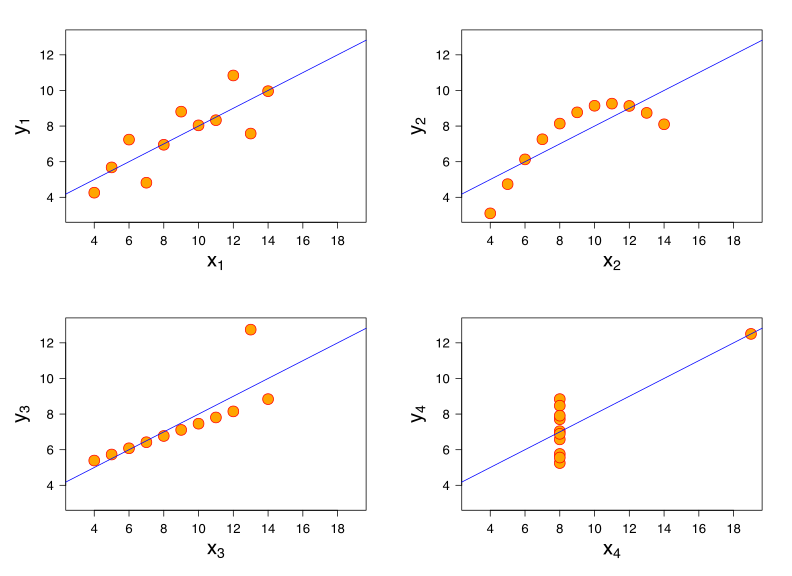
\includegraphics{https://raw.githubusercontent.com/dev7796/data101_tutorial/main/files/img/modeling2/lmvariants.svg}
\caption{Linear models fitted to various different type of data spread. This illustrates the pitfalls of relying solely on a fitted model to understand the relationship between variables. Credits: Wikipedia.}
\end{figure}

\hypertarget{lm}{%
\subsection{Linear regression using lm() function}\label{lm}}

Syntax for building the regression model using the \emph{lm()} function is as follows:

\begin{itemize}
\tightlist
\item
  \texttt{lm(formula,\ data,\ ...)}

  \begin{itemize}
  \tightlist
  \item
    \emph{formula}: here we mention the prediction column and the other related columns(predictors) on which the prediction will be based on.

    \begin{itemize}
    \tightlist
    \item
      \texttt{prediction\ \textasciitilde{}\ predictor1\ +\ predictor2\ +\ predictor3\ +\ ...}
    \end{itemize}
  \item
    \emph{data}: here we provide the dataset on which the linear regression model is to be trained.
  \end{itemize}
\end{itemize}

For more info on the \emph{lm()} function visit \href{https://www.rdocumentation.org/packages/stats/versions/3.6.2/topics/lm}{lm()}

Lets look at the example on the Moody dataset.

\begin{table}

\caption{\label{tab:unnamed-chunk-143}Snippet of Moody Num Dataset}
\centering
\begin{tabular}[t]{rrrr}
\toprule
Midterm & Project & FinalExam & ClassScore\\
\midrule
73 & 8 & 70 & 39.60000\\
61 & 100 & 20 & 68.20000\\
58 & 88 & 38 & 67.00000\\
93 & 41 & 46 & 52.47565\\
85 & 52 & 85 & 68.50000\\
\addlinespace
97 & 48 & 19 & 49.10000\\
26 & 59 & 22 & 41.30000\\
58 & 62 & 25 & 50.10000\\
53 & 56 & 27 & 46.70000\\
66 & 27 & 17 & 34.80494\\
\bottomrule
\end{tabular}
\end{table}

Now we can build a simple linear regression model to predict the ClassScore attribute based on the various other attributes present in the dataset, as shown above.

Since we will be predicting only one attribute values, this model will be called simple linear regression model.

\hypertarget{snippet-1-how-much-do-midterm-project-and-final-exam-count}{%
\subsubsection{Snippet 1: How much do Midterm, Project and Final Exam count?}\label{snippet-1-how-much-do-midterm-project-and-final-exam-count}}

eyJsYW5ndWFnZSI6InIiLCJzYW1wbGUiOiJtb29keU5VTTwtcmVhZC5jc3YoJ2h0dHBzOi8vcmF3LmdpdGh1YnVzZXJjb250ZW50LmNvbS9kZXY3Nzk2L2RhdGExMDFfdHV0b3JpYWwvbWFpbi9maWxlcy9kYXRhc2V0L01vb2R5TlVNLmNzdicpXG5zcGxpdDwtMC43Km5yb3cobW9vZHlOVU0pXG5zcGxpdFxubW9vZHlOVU1UcjwtbW9vZHlOVU1bMTpzcGxpdCxdXG5tb29keU5VTVRyXG5tb29keU5VTVRzPC1tb29keU5VTVtzcGxpdDpucm93KG1vb2R5TlVNKSxdXG4jV2UgdXNlIGxpbmVhciByZWdyZXNzaW9uIHRvICNmaW5kIG91dCB0aGUgd2VpZ2h0cyBvZiAjTWlkdGVybSwgUHJvamVjdCBhbmQgRmluYWwgI0V4YW0gaW4gY2FsY3VsYXRpb24gb2YgdGhlICNmaW5hbCBjbGFzcyBzY29yZS4gRWFjaCBvZiAjdGhlbSBhcmUgc2NvcmVkIG91dCBvZiAxMDAgYW5kICN0aGUgZmluYWwgY2xhc3Mgc2NvcmUgaXMgYWxzbyAjc2NvcmVkIG91dCBvZiAxMDAgYXMgd2VpZ2h0ZWQgI3N1bSBvZiBNaWR0ZXJtLCBQcm9qZWN0IGFuZCAjRmluYWwgRXhhbSBzY29yZXMuXG50cmFpbiA8LSBsbShDbGFzc1Njb3Jlfi4sICBkYXRhPW1vb2R5TlVNVHIpXG50cmFpblxucHJlZCA8LSBwcmVkaWN0KHRyYWluLG5ld2RhdGE9bW9vZHlOVU1Ucylcbm1lYW4oKHByZWQgLSBtb29keU5VTVRzJENsYXNzU2NvcmUpXjIpIn0=

We can see that,

\begin{itemize}
\tightlist
\item
  The summary of the lm model give us information about the parameters of the model, the residuals and coefficients, etc.
\item
  The predicted values are obtained from the predict function using the trained model and the test data.
\end{itemize}

\hypertarget{mse}{%
\subsection{Calculating the Error using mse()}\label{mse}}

As was the simple case in the categorical predictions of the classification models, where we could just compare the predicted categories and the actual categories, this type of direct comparison as an accuracy test won't prove useful now in our numerical predictions scenario.

We don't want to eyeball every time we predict, to find the accuracy of our predictions each row by row, so lets see a method to calculate the accuracy of our predictions, using some statistical technique.

To do this we will use the Mean Squared Error(MSE).

\begin{itemize}
\tightlist
\item
  The MSE is a measure of the quality of an predictor/estimator
\item
  It is always non-negative
\item
  Values closer to zero are better.
\end{itemize}

The equation to calculate the MSE is as follows:

\begin{equation}
MSE=\frac{1}{n} \sum_{i=1}^{n}{(Y_i - \hat{Y_i})^2}
\\ \text{where $n$ is the number of data points, $Y_i$ are the observed value}\\ \text{and $\hat{Y_i}$ are the predicted values}
\end{equation}

To implement this, we will use the \emph{mse()} function present in the Metrics Package, so remember to install the Metrics package and use \texttt{library(Metrics)} in the code for local use.

The syntax for \emph{mse()} function is very simple:

\begin{itemize}
\tightlist
\item
  \texttt{mse(actual,predicted)}

  \begin{itemize}
  \tightlist
  \item
    \emph{actual}: vector of the actual values of the attribute we want to predict.
  \item
    \emph{predicted}: vector of the predicted values obtained using our model.
  \end{itemize}
\end{itemize}

\hypertarget{snippet-2-cross-validate-your-prediction}{%
\subsection{Snippet 2: Cross Validate your prediction}\label{snippet-2-cross-validate-your-prediction}}

eyJsYW5ndWFnZSI6InIiLCJzYW1wbGUiOiJsaWJyYXJ5KE1vZGVsTWV0cmljcylcblxudHJhaW4gPC0gcmVhZC5jc3YoXCJodHRwczovL3Jhdy5naXRodWJ1c2VyY29udGVudC5jb20vZGV2Nzc5Ni9kYXRhMTAxX3R1dG9yaWFsL21haW4vZmlsZXMvZGF0YXNldC9Nb29keU5VTS5jc3ZcIilcbiNzY3JhbWJsZSB0aGUgdHJhaW4gZnJhbWVcbnY8LXNhbXBsZSgxOm5yb3codHJhaW4pKVxudlsxOjVdXG50cmFpblNjcmFtYmxlZDwtdHJhaW5bdiwgXVxuXG4jb25lIHN0ZXAgY3Jvc3N2YWxpZGF0aW9uXG5uIDwtIDEwMFxudHJhaW5TYW1wbGU8LXRyYWluU2NyYW1ibGVkW25yb3codHJhaW5TY3JhbWJsZWQpLW46bnJvdyh0cmFpblNjcmFtYmxlZCksIF1cbnRlc3RTYW1wbGUgPC0gdHJhaW5TY3JhbWJsZWRbMTpuLF1cblxubG0udHJlZSA8LSBsbShDbGFzc1Njb3Jlfi4sICBkYXRhPXRyYWluU2FtcGxlKVxubG0udHJlZVxuXG5wcmVkIDwtIHByZWRpY3QobG0udHJlZSxuZXdkYXRhPXRlc3RTYW1wbGUpXG5wcmVkXG5cbm1zZSh0ZXN0U2FtcGxlJENsYXNzU2NvcmUscHJlZCkifQ==

We can see that,

\begin{itemize}
\tightlist
\item
  The summary of the lm model give us information about the parameters of the model, the residuals and coefficients, etc.
\item
  The predicted values are obtained form the predict function using the trained model and the test data. In comparison to the previous model we are using the cross validation technique to check that if we have more accurate predictions, thus increasing the overall accuracy of the model.
\end{itemize}

\hypertarget{snippet-3-submission-with-lm}{%
\subsection{Snippet 3: Submission with lm}\label{snippet-3-submission-with-lm}}

eyJsYW5ndWFnZSI6InIiLCJzYW1wbGUiOiJsaWJyYXJ5KHJwYXJ0KVxudGVzdDwtcmVhZC5jc3YoJ2h0dHBzOi8vcmF3LmdpdGh1YnVzZXJjb250ZW50LmNvbS9kZXY3Nzk2L2RhdGExMDFfdHV0b3JpYWwvbWFpbi9maWxlcy9kYXRhc2V0L01vb2R5TlVNX3Rlc3QuY3N2JylcbnN1Ym1pc3Npb248LXJlYWQuY3N2KCdodHRwczovL3Jhdy5naXRodWJ1c2VyY29udGVudC5jb20vZGV2Nzc5Ni9kYXRhMTAxX3R1dG9yaWFsL21haW4vZmlsZXMvZGF0YXNldC9NMjAyMnN1Ym1pc3Npb24uY3N2JylcbnRyYWluIDwtIHJlYWQuY3N2KFwiaHR0cHM6Ly9yYXcuZ2l0aHVidXNlcmNvbnRlbnQuY29tL2Rldjc3OTYvZGF0YTEwMV90dXRvcmlhbC9tYWluL2ZpbGVzL2RhdGFzZXQvTW9vZHlOVU0uY3N2XCIpXG5cbnRyZWUgPC0gbG0oQ2xhc3NTY29yZX4uLCAgZGF0YT10cmFpbilcbnRyZWVcblxucHJlZGljdGlvbiA8LSBwcmVkaWN0KHRyZWUsIG5ld2RhdGE9dGVzdClcblxuI05vdyBtYWtlIHlvdXIgc3VibWlzc2lvbiBmaWxlIC0gaXQgd2lsbCBoYXZlIHRoZSBJRHMgYW5kIG5vdyB0aGUgcHJlZGljdGVkIGdyYWRlc1xuc3VibWlzc2lvbiRHcmFkZTwtcHJlZGljdGlvbiBcblxuIyB1c2Ugd3JpdGUuY3N2KHN1Ym1pc3Npb24sICdzdWJtaXNzaW9uLmNzdicsIHJvdy5uYW1lcz1GQUxTRSkgdG8gc3RvcmUgc3VibWlzc2lvbiBhcyBjc3YgZmlsZSBvbiB5b3VyIG1hY2hpbmUgYW5kIHN1YnNlcXVlbnRseSBzdWJtaXQgaXQgb24gS2FnZ2xlIn0=

\hypertarget{MLP}{%
\section{🔖 Machine Learning-Prediction Loop}\label{MLP}}

\begin{itemize}
\tightlist
\item
  \textbf{Lecture slides: } Prediction Loop

  \hypertarget{ML12}{}
\end{itemize}

\hypertarget{BA}{%
\section{🔖 Boundless Analytics}\label{BA}}

\hypertarget{snippet-1-chi-square-hunt}{%
\subsection{Snippet 1: Chi square hunt}\label{snippet-1-chi-square-hunt}}

eyJsYW5ndWFnZSI6InIiLCJzYW1wbGUiOiIjIFNheSwgdGhlIEJvdW5kbGVzcyBhbmFseXRpY3MgcHJvdmlkZXMgdXMgd2l0aCB0aGUgc2xpY2U6ICBCZWVyID09J0xhZ2VyJyAmICBEYXkgPT0nV2Vla2VuZCcgYW5kIFNuYWNrcyA9J0NyYWNrZXJzJyBhbmQgYW5jaG9yIGF0dHJpYnV0ZSBpcyBMb2NhdGlvbi4gIFlvdSBjYW4gY2FsY3VsYXRlIENoaXNxIGZvciB0aGlzIHNsaWNlIGFuZCB0aGUgTG9jYXRpb24gYXR0cmlidXRlIHRvIHRlc3QgaWYgZGlzdHJpYnV0aW9uIG9mIGxvY2F0aW9ucyBpcyBhZmZlY3RlZCBpZiB3ZSBsaW1pdCBvdXJzZWx2ZXMgb25seSB0byB0cmFuc2FjdGlvbnMgc2VsbGluZyBMYWdlciBhbmQgQ3JhY2tlcnMgb24gV2Vla2VuZHM/ICBcblxuIyBUaGUgbW9zdCBpbnRlcmVzdGluZyBzbGljZS1hbmNob3IgYXR0cmlidXRlIGNvbWJpbmF0aW9ucyBhcmUgdGhlIG9uZXMgd2l0aCB0aGUgbGFyZ2VzdCBjaGlzcSB0ZXN0IGFuZCBsb3dlc3QgcC12YWx1ZS4gTmV2ZXJ0aGVsZXNzIGRvIG5vdCBmb3JnZXQgYWJvdXQgbXVsdGlwbGUgaHlwb3RoZXNpcyBjb3JyZWN0aW9uIC0gc2luY2Ugd2UgY2FuIG9uIGNoaS1zcXVhcmUgaHVudCBoZXJlIVxuXG5NaW5pbWFya2V0PC1yZWFkLmNzdihcImh0dHBzOi8vcmF3LmdpdGh1YnVzZXJjb250ZW50LmNvbS9kZXY3Nzk2L2RhdGExMDFfdHV0b3JpYWwvbWFpbi9maWxlcy9kYXRhc2V0L0hvbWV3b3JrTWFya2V0MjAyMi5jc3ZcIilcblxuTWluaW1hcmtldCRJTjwtJ091dF9TbGljZSdcbk1pbmltYXJrZXRbTWluaW1hcmtldCRCZWVyPT0nTGFnZXInICYgTWluaW1hcmtldCREYXk9PSdXZWVrZW5kJyAmICBNaW5pbWFya2V0JFNuYWNrcyA9PSdDcmFja2VycycsIF0kSU48LSdJbl9TbGljZSdcbmQ8LXRhYmxlKE1pbmltYXJrZXQkTG9jYXRpb24sIE1pbmltYXJrZXQkSU4pXG5jaGlzcS50ZXN0KGQpIn0=

\hypertarget{MAD}{%
\section{🔖 How can data fool us?}\label{MAD}}

\begin{itemize}
\tightlist
\item
  \textbf{Lecture Slides: } Unlock Mysteries

  \hypertarget{Mt12}{}
\end{itemize}

\end{document}
